\documentclass[12pt]{article}
\usepackage{geometry}
\geometry{a4paper}
\usepackage[colorlinks, linkcolor=blue, citecolor=blue, urlcolor=blue]{hyperref}
\usepackage[automake]{glossaries-extra}
\usepackage{appendix}
\usepackage{graphicx} % Needed for including images
\usepackage{mdframed} % For creating framed boxes
\usepackage[backend=biber, style=ieee]{biblatex} % Adding biblatex with IEEE style
\usepackage{minted}

\addbibresource{Reference.bib} % Specify the bibliography file, here 'references.bib'


\makeglossaries % 初始化术语表系统

% 定义一些术语
 
\newglossaryentry{opencv}{
    name=OpenCV,
    description={OpenCV (Open Source Computer Vision Library) is a library of programming functions mainly for real-time computer vision. Originally developed by Intel, it was later supported by Willow Garage, then Itseez (which was later acquired by Intel). The library is cross-platform and licensed as free and open-source software under Apache License 2. Starting in 2011, OpenCV features GPU acceleration for real-time operations.\cite{qt}}
}

\newglossaryentry{QT}{
    name=Qt,
    description={Qt (pronounced "cute" or as an initialism) is cross-platform application development framework for creating graphical user interfaces as well as cross-platform applications that run on various software and hardware platforms such as Linux, Windows, macOS, Android or embedded systems with little or no change in the underlying codebase while still being a native application with native capabilities and speed.\cite{cv}}
}

\newglossaryentry{aruco}{
    name=Aruco Marker,
    description={ArUco markers are 2D binary-encoded fiducial patterns designed to be quickly located by computer vision systems. ArUco marker patterns are defined by a binary dictionary in OpenCV, and the various library functions return pattern IDs and pose information from scanned images.\cite{arucomarkers}}
}
\newglossaryentry{vtk}{
      name=VTK,
      description={The Visualization Toolkit (VTK) is an open-source, freely available software system for 3D computer graphics, modeling, image processing, volume rendering, scientific visualization, and 2D plotting. It supports a wide variety of visualization algorithms and advanced modeling techniques, and it takes advantage of both threaded and distributed memory parallel processing for speed and scalability, respectively.\cite{vtkBook}}
}

\newglossaryentry{alpha}{
      name=Alpha Blending,
      description={In computer graphics, alpha compositing or alpha blending is the process of combining one image with a background to create the appearance of partial or full transparency. It is often useful to render picture elements (pixels) in separate passes or layers and then combine the resulting 2D images into a single, final image called the composite. Compositing is used extensively in film when combining computer-rendered image elements with live footage. Alpha blending is also used in 2D computer graphics to put rasterized foreground elements over a background.\cite{Alpha}}
}

\newglossaryentry{aesl}{
      name=Adaptive Exponential Smoothing,
      description={Adaptive exponential smoothing models are designed to improve performance by letting the smoothing parameter vary according to the most recent forecasting accuracy. \cite{aes,aes2}}
}

\newglossaryentry{emal}{
      name=Exponential Moving Average,
      description={An exponential moving average (EMA) is a type of moving average (MA) that places a greater weight and significance on the most recent data points. The exponential moving average is also referred to as the exponentially weighted moving average. An exponentially weighted moving average reacts more significantly to recent price changes than a simple moving average simple moving average (SMA), which applies an equal weight to all observations in the period.\cite{InvestopediaEMA}}
}

\newglossaryentry{cesl}{
      name=Complex Exponential Smoothing,
      description={Complex exponential smoothing is a time series forecasting method that combines exponential smoothing with trend and seasonality. It is a variant of the standard exponential smoothing method, which is a simple technique for smoothing out data by using a weighted average of past observations.\cite{ComplexES2018}}
}


\newglossaryentry{mrtkl}{
      name=Microsoft Mixed Reality Toolkit-Unityde,
      description={MRTK-Unity is a Microsoft-driven project that provides a set of components and features, used to accelerate cross-platform MR app development in Unity. Here are some of its functions: 1.Provides the cross-platform input system and building blocks for spatial interactions and UI. 2.Enables rapid prototyping via in-editor simulation that allows you to see changes immediately. 3.Operates as an extensible framework that provides developers the ability to swap out core components.\cite{MRTKUnity2024}}
}

\newglossaryentry{blender}{
      name=Blender,
      description={Blender is a free and open-source 3D computer graphics software tool set used for creating animated films, visual effects, art, 3D-printed models, motion graphics, interactive 3D applications, virtual reality, and, formerly, video games. Blender's features include 3D modelling, UV mapping, texturing, digital drawing, raster graphics editing, rigging and skinning, fluid and smoke simulation, particle simulation, soft body simulation, sculpting, animation, match moving, rendering, motion graphics, video editing, and compositing\cite{Blender2024,blender}.}
}

\newglossaryentry{holo}{
      name=Microsoft Hololens,
      description={Microsoft HoloLens is an augmented reality (AR)/mixed reality (MR) headset developed and manufactured by Microsoft. HoloLens runs the Windows Mixed Reality platform under the Windows 10 operating system. Some of the positional tracking technology used in HoloLens can trace its lineage to the Microsoft Kinect, an accessory for Microsoft's Xbox 360 and Xbox One game consoles that was introduced in 2010\cite{holo1,holo2}}
}

\newglossaryentry{git}{
      name=GitHub,
      description={GitHub is a developer platform that allows developers to create, store, manage and share their code. It uses Git software, providing the distributed version control of Git plus access control, bug tracking, software feature requests, task management, continuous integration, and wikis for every project. Headquartered in California, it has been a subsidiary of Microsoft since 2018. It is commonly used to host open source software development projects. As of January 2023, GitHub reported having over 100 million developers and more than 420 million repositories, including at least 28 million public repositories. It is the world's largest source code host as of June 2023.\cite{git}}
}

\newglossaryentry{pyside}{
      name=PySide6,
      description={PySide is a Python binding of the cross-platform GUI toolkit Qt developed by The Qt Company, as part of the Qt for Python project. It is one of the alternatives to the standard library package Tkinter. Like Qt, PySide is free software. PySide supports Linux/X11, macOS, and Microsoft Windows. The project can also be cross compiled to embedded systems like Raspberry Pi, and Android devices.\cite{pyside1,pyside2}}
}

% 定义一个缩写词
\newabbreviation{aes}{AES}{
      Adaptive Exponential Smoothing}

\newabbreviation{ema}{EMA}{
      Exponential Moving Average}

\newabbreviation{ces}{CES}{
      Complex Exponential Smoothing}    

\newabbreviation{mrtk}{MRTK}{
      Microsoft Mixed Reality Toolkit-Unity}  

\newabbreviation{rvec}{RVEC}{
            rotation vector}  

\newabbreviation{tvec}{TVEC}{
      translation vector}  

\begin{document}

\begin{titlepage}
      \centering

      \includegraphics[width=0.6\textwidth]{Liverpool.jpg} % Increased width
      \vspace*{1cm}

      \Large
      COMP390

      \large
      2023/24

      \vspace{0.5cm}
      \Huge
      \textbf{Computer Vision and AR for Endovascular Intervention}

      \vspace{1.5cm}


      % Framed box for student information
      \begin{mdframed}
            \normalsize % Smaller text size within the box
            \textbf{Student Name:} [Yulin Huang]\\[20pt] % Name on the same line, add vertical space
            \textbf{Student ID:} [201676465]\\[20pt] % ID on the same line, add vertical space
            \textbf{Supervisor Name:} [Anh Nguyen] % Supervisor on the same line
      \end{mdframed}

      \vspace{2cm} % Adjust space as necessary
      \Large
      \textbf{DEPARTMENT OF}\\
      \vspace{0.1cm} % Adjust line spacing
      \textbf{COMPUTER SCIENCE}

      \vspace{4cm} % Large space as required
      \large
      University of Liverpool\\
      Liverpool L69 3BX


\end{titlepage}
% Acknowledgements page
\newpage
\thispagestyle{empty} % Remove page number from the acknowledgements page
\begin{center}
      \Large \textbf{Acknowledgements}
\end{center}
\vspace{1cm}
\normalsize
%Here for the Acknowledgements
I would like to express my deepest gratitude to my supervisor, Anh Nguyen, for his invaluable guidance and support throughout my research. His insights and expertise have been fundamental to the success of this work.
\\\\
Special thanks also go to Tudor Jianu for his advice and contributions that greatly enhanced this project.
\\\\
I would like to extend my heartfelt thanks to my family. Their unwavering support and love have been my strength and motivation throughout this journey.
\\\\
I am also immensely grateful to my girlfriend, Lucy Zhao, for her understanding and encouragement during the course of my thesis. Her support has been a cornerstone of my personal and academic journey.
\\\\
Furthermore, I wish to acknowledge the critical role played by open-source libraries in the realization of this project. I extend my thanks to the developers of OpenCV\cite{opencv_library} and SciKit-Surgery Augmented Reality\cite{Thompson_SciKit-Surgery_Compact_Libraries_2020} for providing essential tools and references that significantly contributed to my project.
\\\\
This work would not have been possible without the collective support and encouragement from each of these individuals and resources. Thank you.
\newpage
\begin{titlepage}
      \centering


      \includegraphics[width=0.6\textwidth]{Liverpool.jpg} % Increased width
      \vspace*{1cm}

      \Large
      COMP390
      \large
      2023/24

      \vspace{4.5cm}
      \Huge
      \textbf{Computer Vision and AR for Endovascular Intervention}

      \vspace{1.5cm}



      \vspace{4cm} % Adjust space as necessary
      \Large
      \textbf{DEPARTMENT OF}\\
      \vspace{0.1cm} % Adjust line spacing
      \textbf{COMPUTER SCIENCE}

      \vspace{1cm} % Large space as required
      \large
      University of Liverpool\\
      Liverpool L69 3BX

\end{titlepage}
\tableofcontents
\newpage

% Abstract 
\section*{Abstract}
This project is divided into two parts, Part1: Real-world Model Interaction and Tracking and Part2: Endovascular Intervention Simulation. 
\\\\
Part1 includes Real-Time Video Capture and Overlay, which could overlay simulated models on real-world images, such as those captured from live camera or uploaded video. In addition, ArUco marker detection in video frames can be performed and the models can be tracked according to the markers. This process was implemented through the \gls{opencv} library and the SciKit-Surgery Augmented Reality\cite{Thompson_SciKit-Surgery_Compact_Libraries_2020} library in combination with Pyside6. 
\\\\
The goal of the second part was to create an Endovascular Intervention simulation tool for use in Augmented Reality (AR) and Mixed Reality (MR) environments. This part was developed through Unity combined with the \gls{mrtk} development framework.
% Statement of Ethical Compliance
\section*{Statement of Ethical Compliance}
\begin{mdframed}
      \Large % Larger font size for the first two lines
      Data Category: A \\
      Participant Category: 0 \\
      \normalsize % Normal font size for the rest of the text
      I confirm that I have read the ethical guidelines and will follow them during this project. Further details can be found in the relevant sections of this proposal.
\end{mdframed}
\newpage

% Introduction & Background
\section{Introduction \& Background}
This project is dedicated to the development of an open-source simulator of Endovascular Intervention that can be deployed in AR/VR devices, which is designed with two main parts: Part1: Real-world Model Interaction and Tracking and Part2: Endovascular Intervention Simulation.
\\\\
Part1 focuses on the superposition of the model and the real-world scene in the augmented reality environment, and the positioning in the virtual scene, while Part2 focuses on the endovascular intervention simulation, with an emphasis on the interaction of the Catheter and the Aorta walls during the simulation process, and their adaptation to AR/VR devices.
\\\\
The background research for this project is focused on the feasibility and implementation of Endovascular Intervention simulator in VR and AR systems, such as HoloLens. Also for the interaction between the catheter and the aorta during endovascular manipulation. Attention is also given to methods for overlaying display and virtual scenes in AR/VR, and research is desired on performing localisation in virtual environments relative to the display environment.
\\\\
In the past, physics simulations, such as collisions and deformation of objects, were often simulated using the Mujoco platform. MuJoCo Physics Engine are lauded for their ability to orchestrate complex simulations, especially in virtual spaces where high-fidelity interaction is critical\cite{mujoco}. The integration with Unity, further amplifies its capabilities. The combined strengths of MuJoCo and Unity form a comprehensive platform, melding the robust physics simulation of MuJoCo with Unity’s proficiency in real-time rendering and interaction\cite{Juliani2018UnityAG}. 
\\\\
In addition, the emergence of magnetic resonance-safe endovascular robotic platforms and the development of endovascular catheterised robotic systems equipped with magnetically-controlled haptic force feedback demonstrate the direction of the industry towards perceptible force sensing and hyper-realistic feedback in training scenarios.\cite{9376657,Li2022AnEC}
\\\\
The expansion into augmented reality (AR) for surgical applications has also been a significant point of interest in recent literature. The feasibility and benefits of using Microsoft HoloLens for holographic augmented reality in endovascular surgery have been explored, with findings supporting the device’s potential for clinical application\cite{Mialhe2021FeasibilityOT}. Similarly, studies on wearable AR navigation systems for surgical telementoring based on Microsoft HoloLens indicate that such technology could revolutionize surgical education and remote guidance\cite{Liu2020AWA}. The efficiency of marker tracking for surgical navigation using both mono and stereo vision in Microsoft HoloLens underscores the device’s applicability to the medical field\cite{Thabit2022EvaluationOM}. Additionally, the Microsoft HoloLens 2 has been analyzed extensively for its use in medical and healthcare contexts, showing promising prospects for future advancements\cite{Palumbo2022MicrosoftH2}. 

\paragraph{About Specific Terminology or Acronyms}

In order that the general computer science reader can accurately understand any specific terminologies or acronym that appears in this paper, a glossary has been created at the end of the paper and hyperlinks have been used wherever a specific terminology  or acronym appears in the text, which can be clicked on to jump to the corresponding section of the glossary.
\\
 % Add a label to the section that defines the glossary
\hyperref[sec:glossary]{Hyperlink to glossary} % Use the label in the hyperlink
\section{Design \& Implementation}

\subsection{Part1: Real-world Model Interaction and Tracking}
% 这一部分集中讨论与现实世界模型的交互与跟踪的设计和实现。

In this part, I used \gls{opencv}\cite{opencv_library} and SciKit-Surgery Augmented Reality\cite{Thompson_SciKit-Surgery_Compact_Libraries_2020} libraries for image
processing and  model tracking. \gls{QT}\cite{QtWebsite} is used to design the graphical interface, and \gls{vtk}\cite{vtkBook} to build a overlay window\cite{6864541}. OpenCV and SciKit-Surgery libraries help me process images
and track \gls{aruco}\cite{1467495} within video steaming. Qt allows me to create a user interface that ensures  user could more easily change multiple settings, which can enhance the user experience.
VTK and SciKit-Surgery Augmented Reality library are the management of overlay and multi-layer video rendering in my project.
An ArUco Marker Generator is also included, which enables the user to generate different ArUco Markers and save them.
This section will detail the system's design, focusing on System Components and Organization, Data Structures and Algorithms,
User Interface Design, and Design Notation and Diagrams.


\subsubsection{Design}
\begin{enumerate}
      \item \textbf{System Components and Organization}
            \\The project is structured into three primary components, each responsible for distinct functionalities within the system.
            Here’s a detailed breakdown of these components and their organization:
            \begin{enumerate}
                  \item \textbf{Frontend - User Interface}
                        \\The system's user interface is developed using Qt, which is a framework that enables the creation of graphically applications.
                        The main class controlling the UI is \emph{Overlay\_and\_Tracking.py}, which serves as the central hub for user interactions and display functionalities.
                        This class manages the overlay of models on video streaming and provides interactive buttons for users to control various settings, such as model color,
                        video source, models uploading and changing, or adjusting ArUco marker types and sizes, and more.
                  \item \textbf{Backend - Helper Classes}
                        \\The backend is composed of various helper classes, each set to handle specific tasks:
                        \begin{itemize}
                              \item \textit{Image Capture:} The \emph{video\_source.py} class handles the acquisition of video streams from various sources,
                                    including live cameras and recorded media. It is responsible for configuring camera settings, initializing video capture, and video frame cropping to adapted to screen size. This component ensures the reliability and stability of video feed intake.

                              \item \textit{Model Loading:} Managed by \emph{model\_loader.py}, this component is important for the model loading and initializing. It loads ".stl" model files from external files, sets up texture mapping, and prepares the models for real-time overlay. The class also checks for errors in model data to prevent crashes or rendering issues during operation. It also optimizes the structures of model data to enhance rendering efficiency and reduce memory overhead.

                              \item \textit{Model Overlay:} The \emph{overlay\_window.py} is central to integrating 3D models with live or recorded video. With the help of VTK, this module could set up a multi-layered rendering environment where each layer can independently handle elements like video backgrounds, 3D models, or some GUI overlays(In the future, maybe.).

                              \item \textit{Transform Management:} The \emph{transform\_manager.py} class provides a method for managing 4x4 transformation matrices crucial for spatial adjustments of models in 3D space. It stores and retrieves transformations efficiently. And allow it for dynamic modifications of object orientations and positions.

                              \item \textit{ArUco Marker Tracking:} Functionality provided by \emph{arucotracker.py} includes detecting and decoding ArUco markers from the video stream using OpenCV. This module calculates position and orientation of detected marker, and handle the spatial position data for model tracking.
                        \end{itemize}


                  \item \textbf{Additional Component - ArUco Marker Generator}
                        \\An independent component in the system is the ArUco Marker Generator, managed by \emph{Aruco\_Generator.py}.
                        This tool allows users to select and visualize different ArUco markers. Users can also save these markers as separate image files.
            \end{enumerate}
            \paragraph{Organization:\\}
            The system’s architecture is designed to easy maintenance and scalability.
            The modular nature of the helper classes allows for isolated development and testing,
            which enhances the system's robustness and flexibility.
            This organization simplifies development and testing
            and enables the integration of additional functionalities in the future with minimal disruption to the existing system.



      \item \textbf{User Interface Design}
            \\
            In this section, I will show the user interface design of the two main applications of my Part1. Both applications use the Python-based Qt package for user GUI design.
            I will also provide a brief description of the Main menu and the ArUco Marker Generator interface.
            \begin{enumerate}
                  \item \textbf{Main Menu(Overlay and Tracking)}
                        % 描述主菜单的设计和功能。
                        \begin{figure}[H]
                              \centering
                              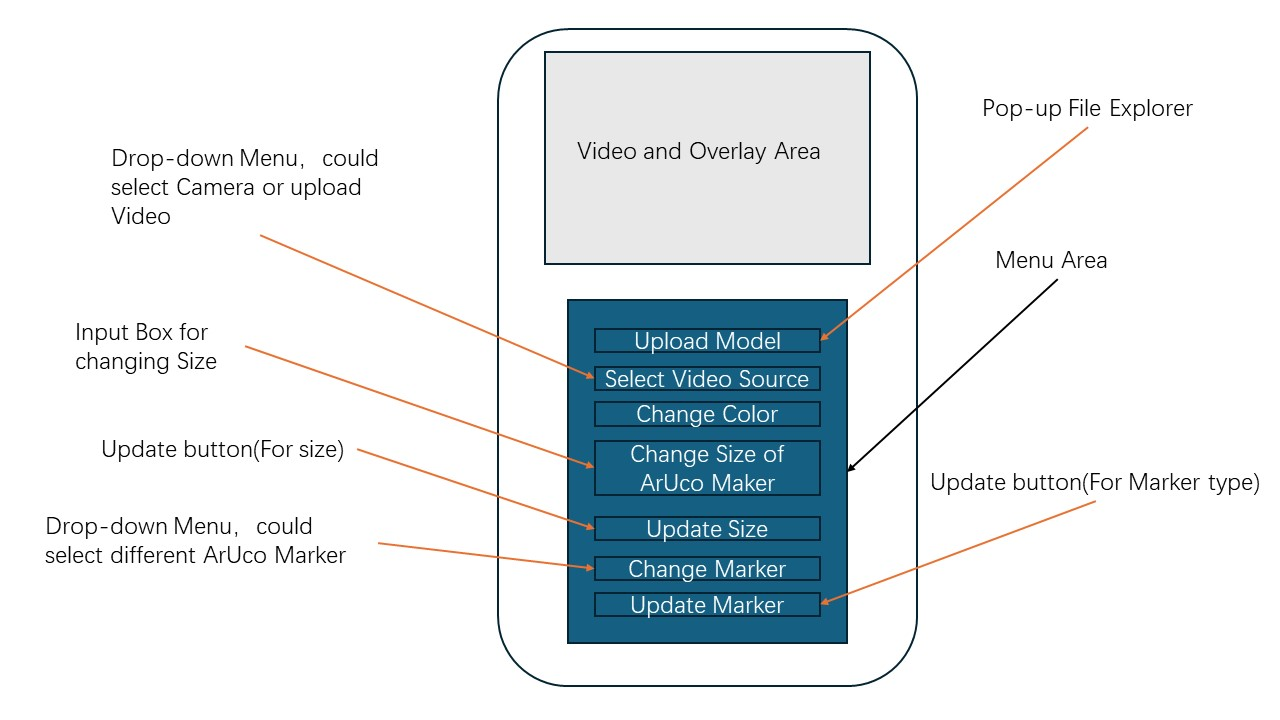
\includegraphics[width=1.2\textwidth]{design_overlay.jpg}
                              \caption{Design of Overlay and Tracking Main Menu}
                        \end{figure}


                        The main menu of Overlay and Tracking is the central hub of the application, providing users with access to all the functionalities.
                        The Main Menu consists of the Video and Overlay Area, which displays the video image and overlay of the model, and the Menu Area, which is responsible for setting various parameters.
                        The menu includes buttons for model uploading, video source selection, ArUco marker settings, and model color adjustments.
                        \\\\
                        When you click on the "Upload Model" button, a file explorer will pop up to select the folder where you want to upload the model. The program will read two files in the folder, one is the model file in ".stl" format, and the other is a file named "colours.txt". the first field in the txt file is the file name of the model, and the last three fields are The first field in the txt file is the file name of the model, and the last three fields are the RGB data of the default colours of the model (the model colours can be changed in the application interface after uploading). After uploading the model will be overlayed onto the video display as Overlay. The second button is the video source selection button, when clicked, a drop-down menu with three options will appear, "Camera1", "Camera2" and "Upload Video Camera1", "Camera2" and "Upload Video". The app will default to "Camera1" as the video source when it is initially launched. Selecting "Camera1" or "Camera2" will directly switch to the corresponding video source. After selecting the "Upload Video" option, an "Upload Video File" button will appear at the bottom. Clicking on the "Upload Video File" button will start the file explorer, you can select ".mp4", ".avi", ".webm" format video for uploading. After the video has been uploaded the tracking of Overlay and ArUco markers will start automatically if there is already an uploaded model present. Similarly, the video source can be switched back to the Camera input by selecting Camera1. After uploading the model, you can change the colour of the model by clicking the "Change Model Color" button.
                        \label{sec:upload}
                        \\\\
                        To ensure the accuracy of ArUco marker tracking, you need to modify the "ArUco Dictionary" to the corresponding dictionary of the marker you are using and click "Update ArUco "button. You also need to change the "ArUco Marker Size", which represents the size of the real ArUco marker in millimetres, and click the "Update Marker Size" button when you are done.

                  \item \textbf{ArUco Generator}
                        % ArUco生成器设计图
                        \begin{figure}[H]
                              \centering
                              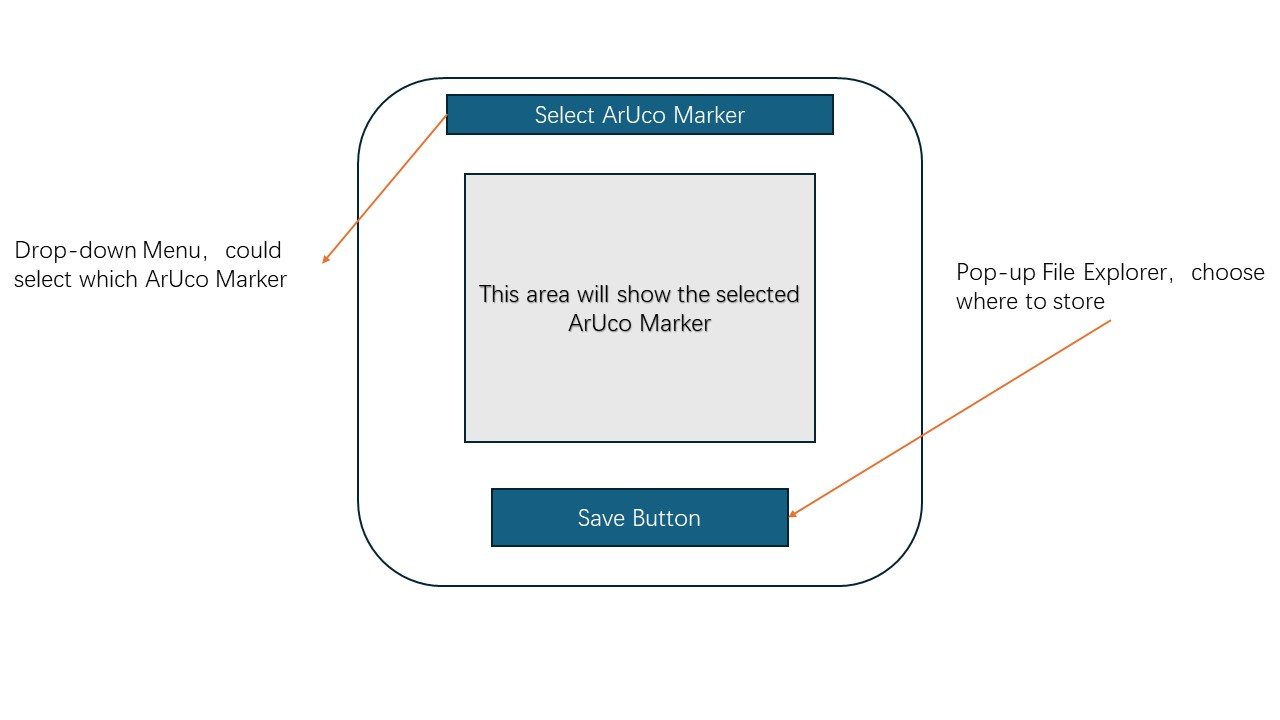
\includegraphics[width=1.2\textwidth]{design_generator.jpg}
                              \caption{Design of ArUco Generator}
                        \end{figure}
                        % 描述ArUco生成器的设计和功能。
                        \begin{figure}[H]
                              \centering
                              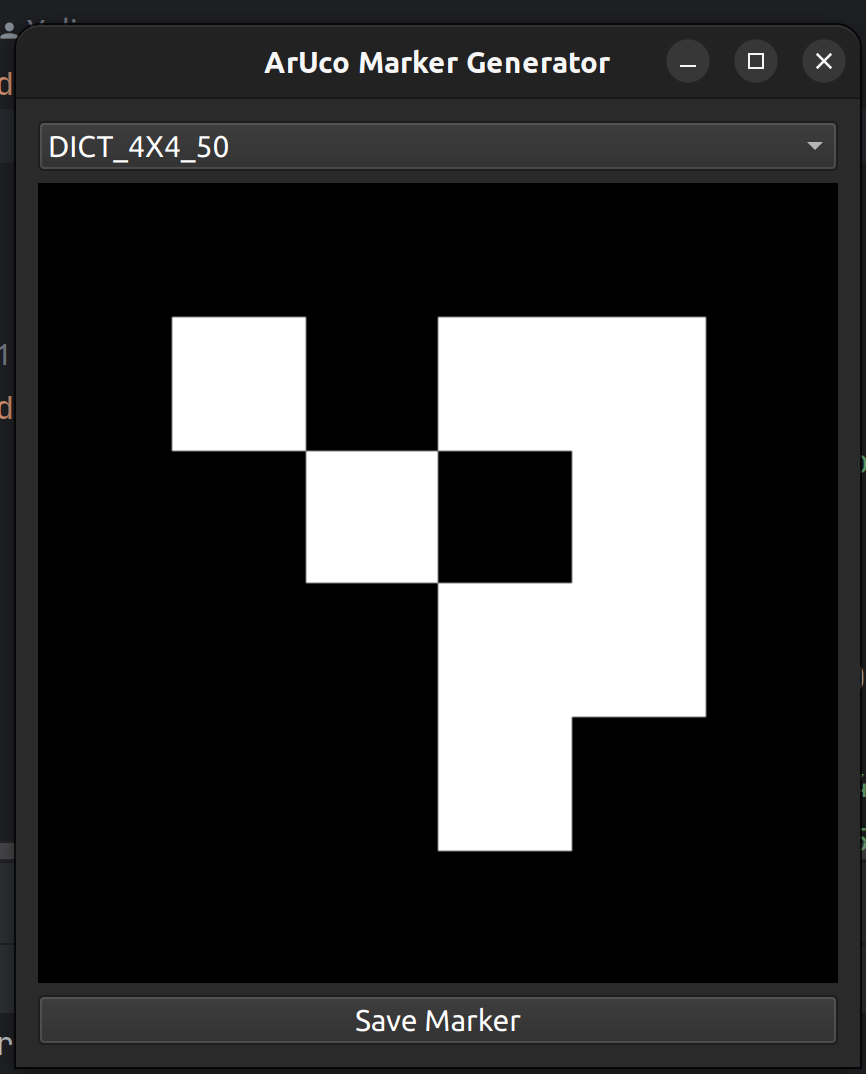
\includegraphics[width=0.4\textwidth]{main_arucuo.png}
                              \caption{ArUco Generator}
                        \end{figure}
                        The ArUco Generator interface allows users to select different ArUco markers from a predefined list and visualize them in real-time.
                        The interface provides a clear preview of the selected marker and allows users to save the marker as an image file for later use.
                        The design is simple and user-friendly, with intuitive controls for easy marker customization.
                        \\\\
                        You can first select the ArUco marker you want to use by launching the drop-down menu via "Select Aruco" and the selected ArUco marker will be displayed on the screen in real time. After that, you can click the "Save Marker" button to start the file explorer to save the marker, the file name will be set to the corresponding dictionary of the ArUco marker by default.
            \end{enumerate}


      \item \textbf{Design Notation and Diagrams}
            \begin{enumerate}
                  \item \textbf{Use Case Diagrams}
                        \begin{figure}[H]
                              \centering
                              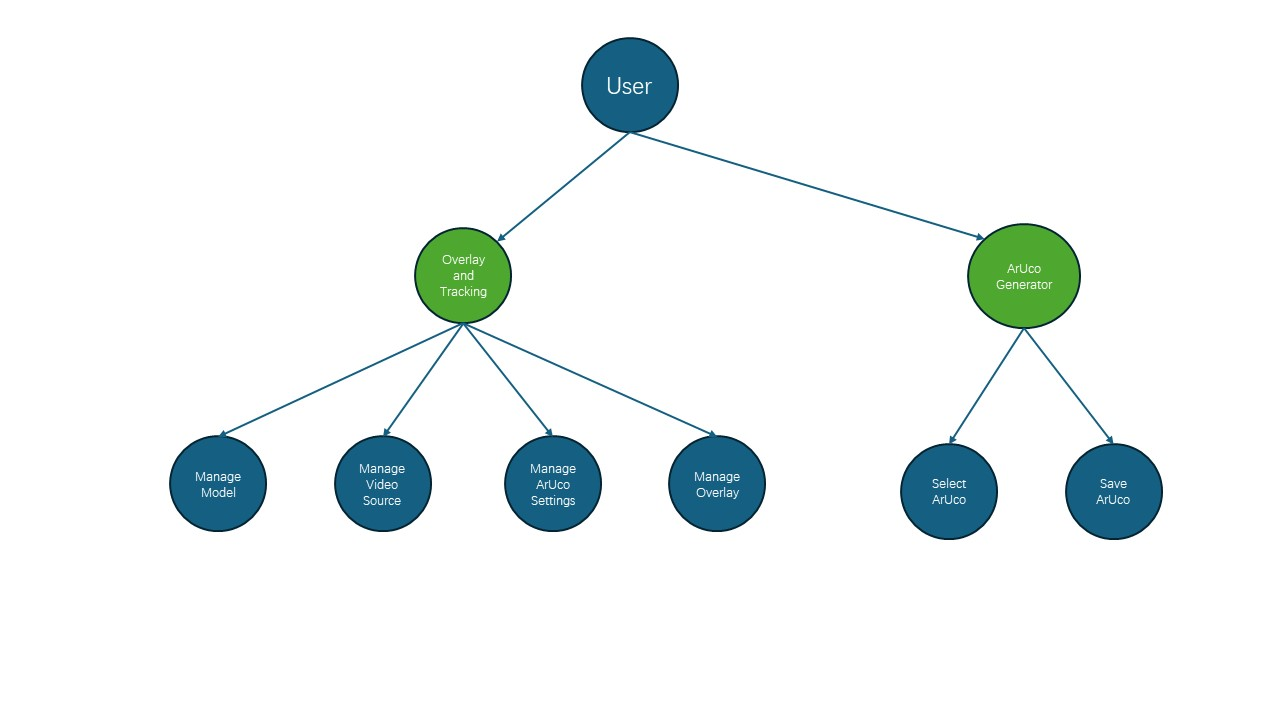
\includegraphics[width=1.1\textwidth]{case.jpg}
                              \caption{Use Case Diagrams}
                        \end{figure}
                  \item \textbf{Data Flow Diagrams}
                        % 提供系统关键部分的伪代码及数据流图。
                        \begin{figure}[H]
                              \centering
                              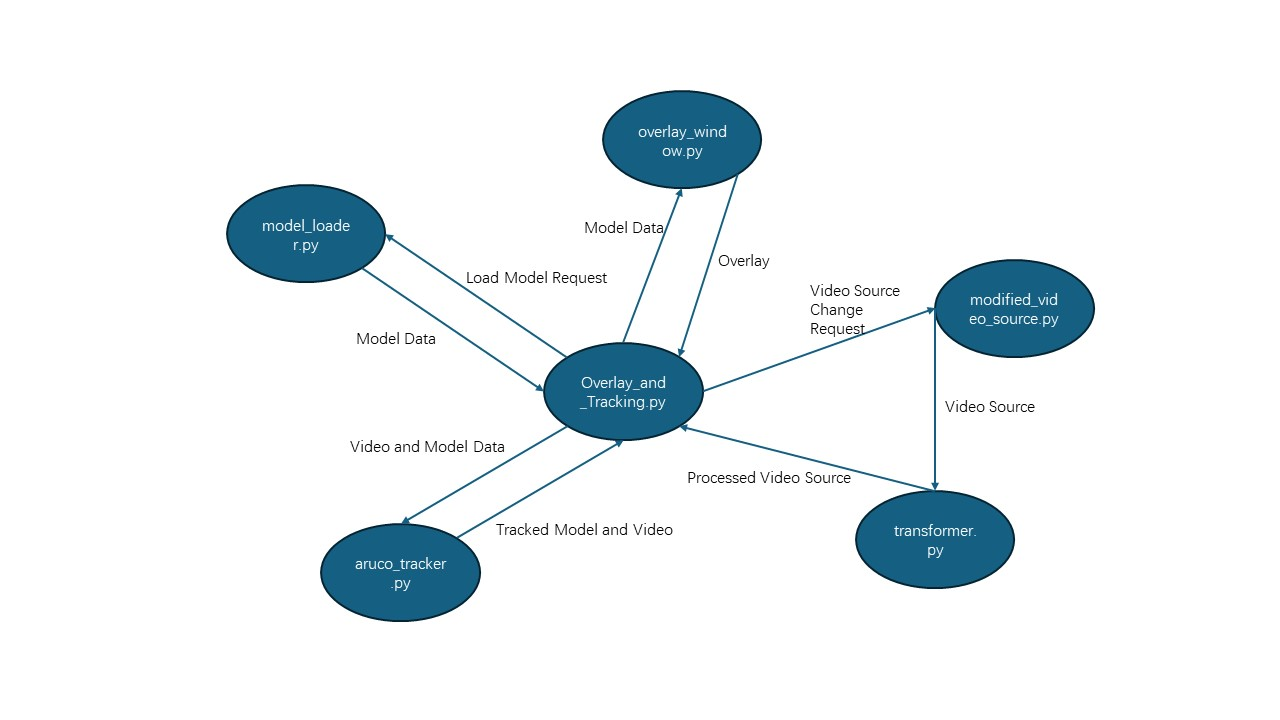
\includegraphics[width=1.1\textwidth]{data.jpg}
                              \caption{Data Flow Diagrams}
                        \end{figure}
            \end{enumerate}
\end{enumerate}

\subsubsection{Implementation}
\begin{enumerate}

      \item \textbf{Backend Implementation}
      \label{sec:backend}
            % 详细说明系统所使用的数据结构和算法。
            \begin{enumerate}
                  \item \textbf{Pre-processing for video capture and upload}
                        \\\\
                        This part is mainly controlled by \emph{video\_source.py} and is combined with a front-end Qt-based user interface to manage the core video processing functions. A robust video source management and processing system is implemented in \emph{video\_source.py} through the \emph{TimestampedVideoSource} class and \emph{VideoSourceWrapper} class. The system allows the user to interactively control the selection of video sources through a graphical interface, and it ensures accurate video stream processing.
                        \begin{itemize}
                              \item \textit{Video Source Configuration and Management:}
                                    \\
                                    The \emph{TimestampedVideoSource} class uses the OpenCV library's, emph{cv2.VideoCapture} method to initialise the video capture from the camera number or file path. It can support basic video capture functionality or provide the ability to validate the size of the video stream to ensure that the resolution is compatible with the system. If the resolution size provided by the setting is valid, the system sets the resolution accordingly. If the resolution is not valid, the system uses the camera's settings by default. If the requested resolution option is not supported by the camera, the system throws an error, which effectively prevents runtime problems that may result from unsupported video configurations and increases system stability and reliability.
                              \item \textit{Synchronisation and Timestamping:}
                                    \\
                                    The \emph{TimestampedVideoSource} class also serves to synchronise the video stream with the modelled overlay, embedding a timestamp with the current date and time at each frame captured. Each time a video frame is successfully read, the \emph{datetime.datetime.now()} method gets the current system time. This timestamp is then converted to a string or other format and stored or passed along with the video frame, ensuring that each frame has an exact timestamp. In Augmented Reality (AR) or Virtual Reality (VR) systems, quasi-timestamping this timestamp ensures alignment between the 3D model and the actual environment.With such a timestamping feature, \emph{TimestampedVideoSource} can ensure the synchronisation of the video frames for the subsequent synchronisation of the model overlay.
                              \item \textit{Handles multiple video sources:}
                                    \\
                                    The \emph{VideoSourceWrapper} class manages multiple video sources, allowing the addition of camera inputs or the uploading of video files, and verifying their existence and compatibility. A centralised method for releasing all video sources is provided in this class to ensure that resources that are no longer needed are managed and cleaned up in a timely manner. Each video source is encapsulated in an instance of the \emph{TimestampedVideoSource } class, which allows each source to be controlled and processed independently. This feature ensures that the system load is at an appropriate level.
                              \item \textit{Retrieve and display video frames:}
                                    \\
                                    Retrieval of frames is achieved by system calls to the \emph{read()} method of each video source, which is implemented through OpenCV's \emph{ cv2.VideoCapture.read() }. This method captures a single frame from the video source and checks to see if it was successfully captured. If successfully captured, the frame is tagged using the current timestamp, ensuring that each frame has an accurate time reference. When processing multiple video sources, the system ensures synchronisation between frames. Synchronisation of frames is achieved by using the same frame rate setting for all sources and matching frames from different sources with timestamps. This allows for smoothness and synchronisation in the case of multiple video source inputs.
                        \end{itemize}

                        \paragraph{pseudocode for the \emph{video\_source.py}:}
                        \begin{minted}[frame=single, linenos=true, fontsize=\footnotesize]{python}
Class TimestampedVideoSource:
    Initialize(source_num_or_file, optional dims):
        Try:
            Open video source with cv2.VideoCapture(source_num_or_file)
        If source not opened:
            Raise RuntimeError("Failed to open Video camera")

        If dimensions provided:
            Validate and set video resolution:
                Check if dimensions are integers and >= 1
                Set resolution using cv2.VideoCapture properties
                If resolution setting fails:
                    Raise ValueError("Requested resolution not supported")

        Initialize empty frame array based on video dimensions
        Initialize timestamp

    Read():
        Capture frame and current time using cv2.VideoCapture.read()
        If frame captured successfully:
            Update timestamp with current datetime
        Return frame, timestamp

    Release():
        Release video source using cv2.VideoCapture.release()

    Update source(new_source):
        Release current source
        Reinitialize with new source

Class VideoSourceWrapper:
    Initialize():
        Create an empty list for storing video sources

    Add camera(camera_number, optional dims):
        Validate camera input (check if camera number is valid)
        Add camera source with optional dimensions to the list

    Add file(filename, optional dims):
        Validate if filename exists and is a valid file
        Add file source with optional dimensions to the list

    Get next frames():
        For each source in the list:
            If source is opened:
                Read frame from source
            Collect and return all frames

    Release all sources():
        For each source in the list:
            Release source
                        \end{minted}
                        % 视频源切换截图展示
                        \begin{figure}[H]
                              \centering
                              \includegraphics[width=0.4\textwidth]{stream_change.jpg}
                              \caption{Video Source Switching}
                        \end{figure}
                        \begin{figure}[H]
                              \centering
                              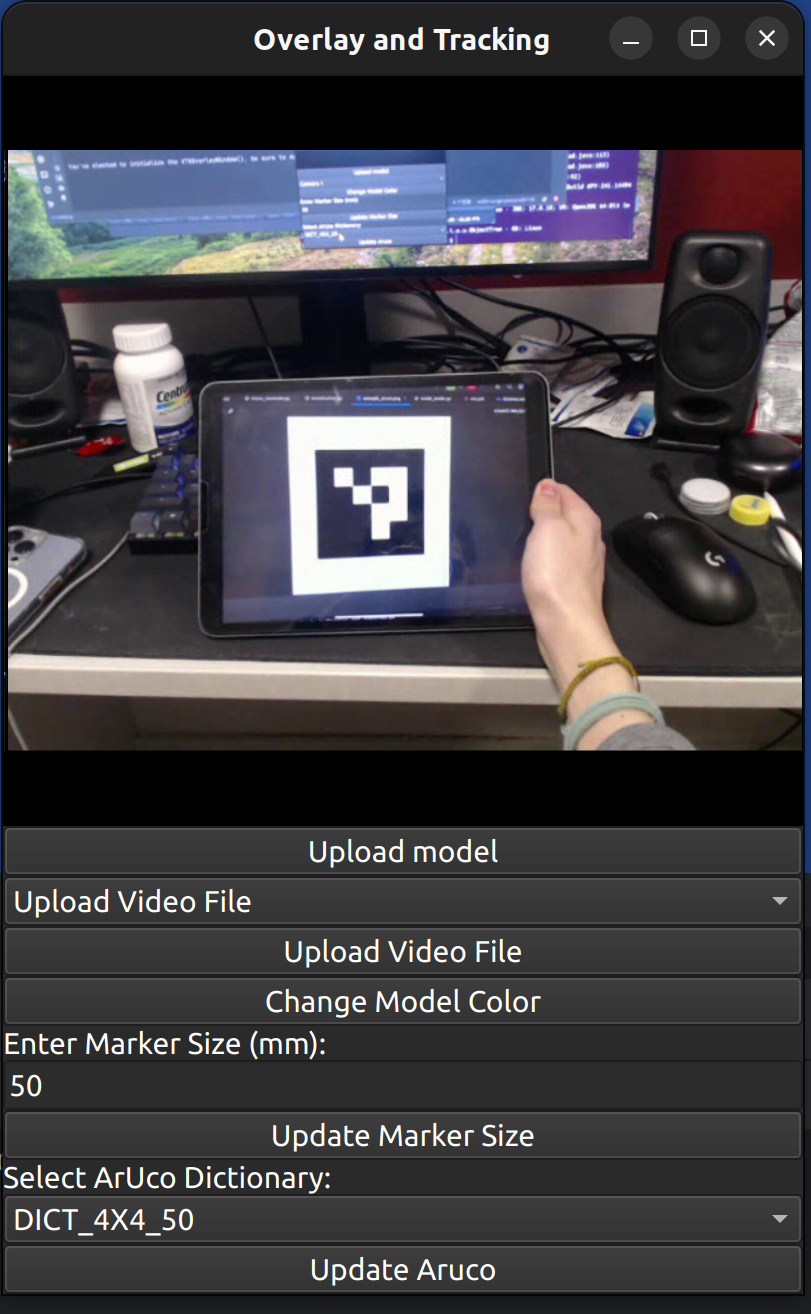
\includegraphics[width=0.4\textwidth]{vedio.png}
                              \caption{Video Upload}
                        \end{figure}
                  \item \textbf{Image Processing Algorithms in Multi-Layer Video Rendering}
                        % 描述如何存储和处理连续的图像帧,例如使用循环缓冲区或队列来管理实时视频帧。
                        \\ In a video rendering system, video frames need to be dynamically managed to create complex visual effects, such as models and real-time video overlays in this project. This also involved real-time adjustments to the \gls{alpha}\cite{Alpha} and video. A greyscale image with alpha blending of the RGBA stream was used to precisely control transparency and layering effects to enable the superimposition of a layer's frame (e.g. the model) onto the original frame\cite{9979846}. Ensuring overlay accuracy and visual fidelity is crucial for applications such as augmented reality\cite{SETTIMI2022104272}.
                        \\\\
                        In addition, it is necessary to update and align the video frames to the appropriate layers by adjusting the data range according to the size of the incoming video frames. This incorporation of real-time processing improves the continuity of the video image by preventing visual interruptions caused by frame misalignment\cite{Wang}.
                        \\\\
                        I also introduced \gls{aesl} into the multi-layer video rendering system (\emph{Overlay\_and\_Tracking.py}). This enhances image processing, such as when processing video streams involving complex dynamic scenes\cite{7410724}. By dynamically adjusting its smoothing parameter (Alpha), \gls{aes} is able to more accurately adapt to changes in content within a video frame, such as lighting adjustments, scene switching, or object movement, and can reduce visual jitter and blurring due to rapid changes \cite{7410724}.
                        \\\\
                        Compared with the traditional \gls{emal}, the adaptive feature of AES has a greater advantage. \gls{ema}, although fast in processing and low in computational cost, may not be able to adequately adapt its fixed smoothing parameters to real-time changes in the video content in the face of complex scene variations, thus affecting the final image quality\cite{aes,aes2,InvestopediaEMA}.
                        In a multilayer rendering system, combining AES for real-time video transmission and dynamically adjusting the smoothing parameters according to the content differences between the previous and previous frames can maintain the continuity and naturalness of the visual effects, especially when dealing with moving objects and changing backgrounds. In addition, AES's also better handles scenes with large lighting variations, maintaining the balance of colors and shades of light and dark \cite{7298776}.
                        \\\\
                        I have similarly experimented with \gls{cesl}, and while it excels in handling data with clear trends and cyclical variations, its application in video rendering systems may not be as straightforward and effective as AES. Because \gls{ces} is designed to provide a more comprehensive understanding of the multiple influences on the data \cite{ComplexES2018,Complex}, its use in non-predictive applications may lead to overly complex processing and increased computational burden.
                        \\\\
                        Therefore, AES is ultimately used in video rendering systems to respond more directly to real-time changes in video content, reduce visual jitter, and improve the viewing experience.
                        \\\\
                        To summarize, AES can improve image stability and visual quality, as well as enhance the system's responsiveness to environmental changes. By intelligently adjusting processing parameters, AES helps to ensure high efficiency while also adapting to visual jitter or lighting changes that may be encountered with ArUco marker tracking.
                        \paragraph{Code for the AES:}
                        \begin{minted}[frame=single, linenos=true, fontsize=\footnotesize]{python}
class SmoothedTransform:
    def __init__(self, alpha, min_alpha=0.01, max_alpha=0.9):
        """
        Initializes the adaptive smoothing transform class.
        
        Parameters:
        alpha (float): The initial smoothing factor.
        min_alpha (float): The minimum allowable value for alpha 
        to prevent it from becoming too low.
        max_alpha (float): The maximum allowable value for alpha 
        to prevent it from becoming too high.
        """
        self.alpha = alpha
        self.min_alpha = min_alpha
        self.max_alpha = max_alpha
        self.transform = None
      def adjust_alpha(self, new_transform):
            """
            Adjusts the smoothing factor alpha based on the 
            difference between the new transform and the 
            current transform to 
            better adapt to recent data changes.
                                          
            Parameters:
            new_transform (float): The new data point used to 
            update the transform.
            """
            if self.transform is not None:
            # Calculate the absolute difference between the current 
            # and new transforms
            error = abs(new_transform - self.transform)
            # Dynamically adjust alpha based on the error, 
            # inversely scaling it
            self.alpha = max(self.min_alpha, min(self.max_alpha, 
            1 / (1 + error)))
                              
      def update(self, new_transform):
            """
            Updates the current transform with a new data point using
            adaptive exponential smoothing.
                                          
            Parameters:
            new_transform (float): The new data point to incorporate
            into the smoothed data.
                                          
            Returns:
            float: The updated transform value.
            """
            if self.transform is None:
            # If no transform has been set yet, initialize it 
            # with the new transform
            self.transform = new_transform
            else:
            # Adjust alpha based on the new data point
            self.adjust_alpha(new_transform)
            # Apply the adjusted alpha to compute 
            # the new smoothed transform
            self.transform = self.alpha * new_transform + 
            (1 - self.alpha) * self.transform
            return self.transform
                              \end{minted}
                        \begin{figure}[H]
                              \centering
                              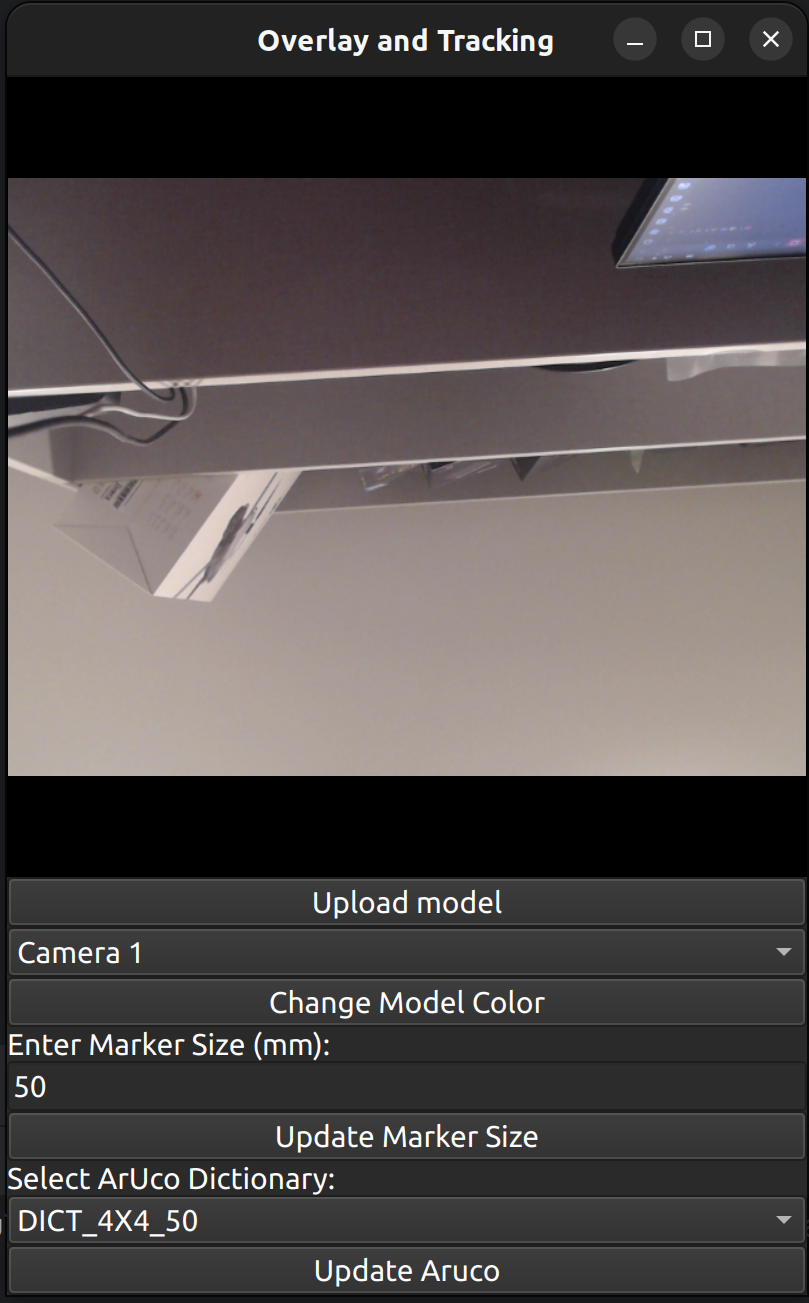
\includegraphics[width=0.4\textwidth]{main_page.png}
                              \caption{Overlay and Tracking Main Menu(Without Overlay Activated)}
                        \end{figure}
                  \item \textbf{Model Rendering and Overlay}
                        % 详述用于检测和追踪ArUco标记的算法,包括图像分割、模式识别和机器学习技术。
                        \\
                        It is mainly implemented by \emph{overlay\_window.py}, in which the \emph{VTKOverlayWindow} class combines the functionality of VTK, Qt and OpenCV for real-time video streaming and model overlay.
                        \begin{itemize}
                              \item \textit{Multi-layer rendering settings for video and models:}
                                    \\
                                    When initialising the \emph{VTKOverlayWindow} class, the VTK library's \emph{vtkRenderWindow} and \emph{vtkRenderer} are used to build a multi-layered rendering environment\cite{7783818}. This multi-layer architecture allows independent control of content rendering on each layer, where the bottom layer is typically used to display live or pre-recorded video, while the top layer is used to add 3D models and other GUI elements\cite{5974642,6194820}. Such a layer setup ensures proper visual overlay between the rendered elements. The \emph{SetNumberOfLayers} method is used to define the number of layers in the rendering window, and the \emph{SetLayer} method is used to assign each renderer to a specific layer. This layering system ensures that the video stream and 3D models are correctly displayed and overlaid in the final output\cite{7783818}.
                                    \paragraph{Code for the multi-layer rendering settings:}
                                    \begin{minted}[frame=single, linenos=true, fontsize=\footnotesize]{python}
# Create a rendering window and set multiple layers
renderWindow = vtk.vtkRenderWindow()
renderWindow.SetNumberOfLayers(3)

# Create renderers for each layer
videoRenderer = vtk.vtkRenderer()
videoRenderer.SetLayer(0)  # Bottom layer for video
modelRenderer = vtk.vtkRenderer()
modelRenderer.SetLayer(1)  # Middle layer for 3D models
uiRenderer = vtk.vtkRenderer()
uiRenderer.SetLayer(2)  # Top layer for UI components

# Add renderers to the rendering window
renderWindow.AddRenderer(videoRenderer)
renderWindow.AddRenderer(modelRenderer)
renderWindow.AddRenderer(uiRenderer)
                              \end{minted}

                              \item \textit{Import and format conversion of video streams:}
                                    \\
                                    In order to implement VTK overlay, the video frames captured by OpenCV need to be converted into a format that VTK can handle. Here the video frames are converted by using VTK's \emph{vtkImageImport} method. The conversion process requires setting the correct data types and sizes and updating the memory pointers to the video frames to ensure that the video stream data captured from OpenCV can be integrated into the VTK rendering process. This ensures synchronisation and integrity of the video stream before and after conversion without causing video lag in VTK.\cite{vtk_image_import_doc,vtk_image_import_2023}
                                    \paragraph{Code for the video stream conversion:}
                                    \begin{minted}[frame=single, linenos=true, fontsize=\footnotesize]{python}
# Initialize video capture
cap = cv2.VideoCapture(0)

# Read a frame from OpenCV and import it into VTK
ret, frame = cap.read()
vtkImage = vtk.vtkImageData()
vtkImage.SetDimensions(frame.shape[1], frame.shape[0], 1)
vtkImage.SetScalarTypeToUnsignedChar()

# Create a VTK image importer and connect it to the image data
imageImporter = vtk.vtkImageImport()
imageImporter.SetInputData(vtkImage)
imageImporter.SetImportVoidPointer(frame.data, frame.nbytes)
imageImporter.Update()
                              \end{minted}
                              \item \textit{Dynamic rendering and adjustment of 3D models:}
                                    \\
                                    Rendering of 3D models is achieved by using components such as VTK's \emph{vtkActor} and \emph{vtkPolyDataMapper}. These components support loading models from external files (e.g. STL format) and allow transformations such as translation, scaling, rotation, etc. to be applied to the model. These transformations of the model can be adjusted in real time to support dynamic user interaction and visual modifications\cite{6037214}. The model can be rendered in the VTK overlay by using the \emph{vtkPolyDataMapper} map the model data to geometry and set the actor using the \emph{vtkActor} and \emph{AddActor} method to add the model to the corresponding rendering layer. Then can use the \emph{SetPosition} and \emph{SetOrientation} method to adjust the model position and orientation to match the video\cite{5357714}.The function of modifying the position of the model will play an important role in section (f) Marker Detection and Tracking.
                                    \paragraph{Code for the dynamic rendering and adjustment of 3D models:}
                                    \begin{minted}[frame=single, linenos=true, fontsize=\footnotesize]{python}
# Load a 3D model from a file
modelReader = vtk.vtkSTLReader()
modelReader.SetFileName("model.stl")

# Map the model data to geometry
mapper = vtk.vtkPolyDataMapper()
mapper.SetInputConnection(modelReader.GetOutputPort())

# Create an actor for the model and add it to the renderer
actor = vtk.vtkActor()
actor.SetMapper(mapper)
modelRenderer.AddActor(actor)

# Adjust model position and orientation to match the video
# The position data can be varied depending on 
# tracking data in (f) Marker Detection and Tracking
actor.SetPosition(10, 0, 0)
actor.SetOrientation(0, 90, 45)
                              \end{minted}
                        \end{itemize}
                        % Overlay截图展示
                        \begin{figure}[H]
                              \centering
                              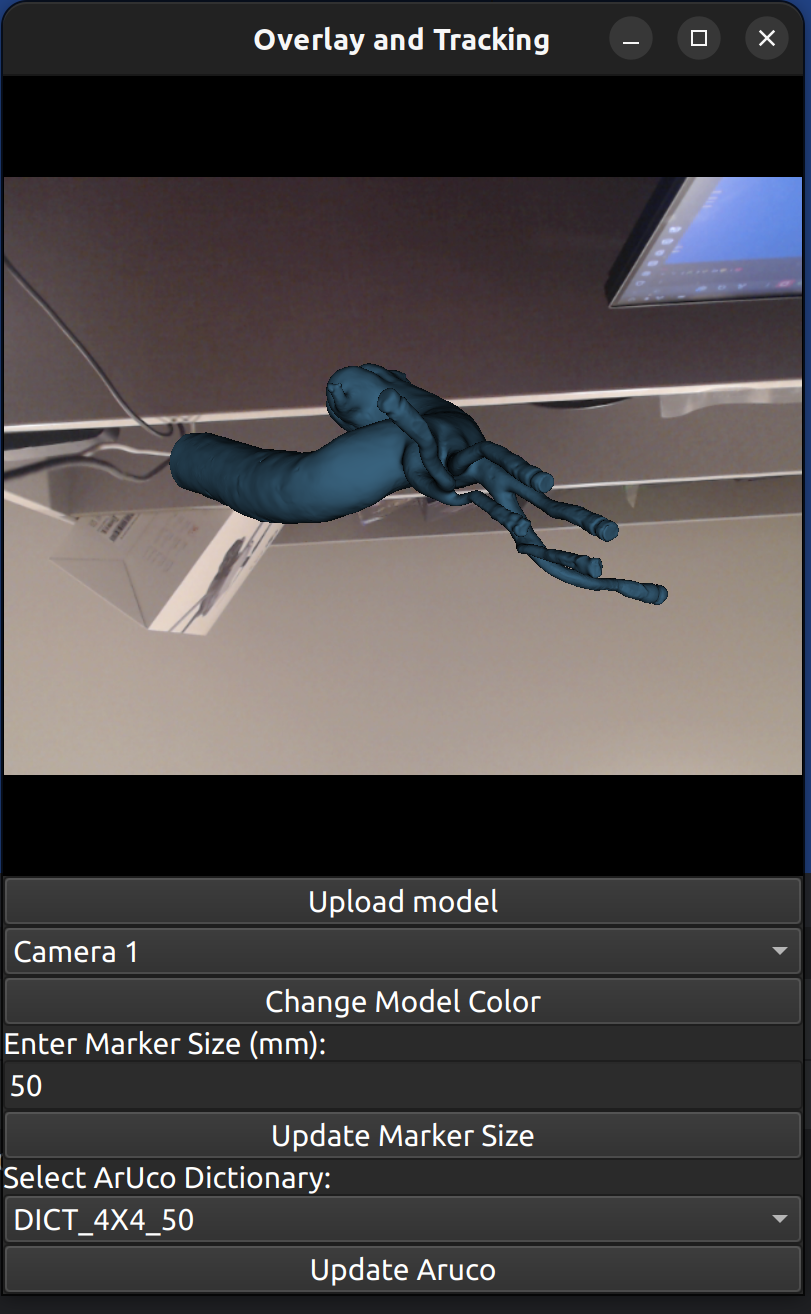
\includegraphics[width=0.4\textwidth]{overlay.png}
                              \caption{Overlay and Tracking Main Menu(With Overlay Activated)}
                        \end{figure}
                  \item \textbf{Optimization of Visual Effects and Depth Processing:}
                        \\
                        To enhance the visual quality of rendering, VTK's Depth Stripping technology can be enabled. Depth peeling is suitable for rendering transparent or semi-transparent objects and effectively solves visual artefacts and incorrect transparency problems during rendering. Through layer-by-layer rendering and compositing, Depth Stripping ensures visual correctness and is suitable for use in complex overlay or multi-object scenes.\cite{vtk_dualdepth_2016,5357714} The \emph{UseDepthPeelingOn} method is used to enable Depth Stripping, and the \emph{SetMaximumNumberOfPeels} and \emph{SetOcclusionRatio} methods are used to set the maximum number of peels and the occlusion ratio, respectively, to control the rendering quality and performance.
                        \paragraph{Code for Optimization of Visual Effects and Depth Processing:}
                        \begin{minted}[frame=single, linenos=true, fontsize=\footnotesize]{python}
# Enable depth peeling for better transparency handling
modelRenderer.UseDepthPeelingOn()
modelRenderer.SetMaximumNumberOfPeels(100)
modelRenderer.SetOcclusionRatio(0.1)
                        \end{minted}
                  \item \textbf{Precise Control of Camera and Viewing:}
                        \label{sec:precise}
                        \\
                        During the implementation of model overlay using VTK, it is important to maintain an accurate overlay between the 3D model and the background video stream. When using different cameras, deviations in the model overlay may occur due to different camera parameters such as focal length, projection, and position. In order to make the model appear accurately at the right position in the background video, the parameters of the camera should be modified. By getting the camera's focal length, position and projection parameters to modify the variables in video processing, the viewpoint between the 3D model view and the video stream background can be consistently matched when using a camera with different characteristics. It might be necessary to additionally adjust the cropping range and field of view of the camera to ensure the correct range of visual output. The \emph{vtkCamera} class is built to control the camera settings. Method like \emph{SetPosition}, \emph{SetFocalPoint}, and \emph{SetViewUp} are used to adjust the camera's position, focus point, and view direction, respectively.\cite{vtk_examples_camera,vtk_camera_doc_2023}
                        \paragraph{Code for Precise Control of Camera and Viewing:}
                        \begin{minted}[frame=single, linenos=true, fontsize=\footnotesize]{python}
# Configure the camera to match the video view
camera = modelRenderer.GetActiveCamera()
camera.SetPosition(0, 0, 100)
camera.SetFocalPoint(0, 0, 0)
camera.SetViewUp(0, 1, 0)
                        \end{minted}
                  \item \textbf{Marker Detection and Tracking}
                        % 介绍如何将三维模型精确地放置在虚拟环境中,可能涉及计算几何和物体识别算法。
                        \begin{itemize}
                              \item \textit{Loading Calibration Data:}
                                    \\
                                    Obtaining accurate camera calibration data before performing the spatial localisation of the model is necessary. It is first necessary to load the projection matrix and distortion coefficients of the camera in \hyperref[sec:precise]{(e) Precise Control of Camera and Viewing}, which have been acquired and stored in that section. This data is then read to calibrate the subsequent image processing and marker recognition so that it accurately reflects the actual camera viewing angle. The use of different calibration data affects the model's spatial localisation function and marker tracking accuracy.
                                    \paragraph{Pseudocode for the Loading Calibration Data:}
                                    \begin{minted}[frame=single, linenos=true, fontsize=\footnotesize]{python}
Function _load_calibration(textfile):
    Read 'projection_matrix' from  
    '(e) Precise Control of Camera and Viewing'
    Read 'distortion' from 
    '(e) Precise Control of Camera and Viewing'
    Return projection_matrix, distortion
                              \end{minted}
                              \item \textit{Initializing Video Source and Tracker Configuration:}
                                    \\
                                    Afterwards, the camera is initialised and the required tracking parameters are set according to the camera configuration obtained in the first step. This includes setting the video source selected by the user (e.g., camera or video file) and configuring the properties of the video stream (e.g., resolution and frame rate.). In addition, the associated rigid body is set up based on the acquired configuration information and the rigid body is used to compute its position and orientation based on the detected markers.
                                    \paragraph{Pseudocode for the Initializing Video Source and Tracker Configuration:}
                                    \begin{minted}[frame=single, linenos=true, fontsize=\footnotesize]{python}
Method initialize_video_capture(video_source, configuration):
    If video_source is not 'none':
        self._capture = cv2.VideoCapture(video_source)
        If "capture properties" in configuration:
            For each property in configuration["capture properties"]:
                self._capture.set(cv2 property, value)
                              \end{minted}
                              \item \textit{Load ArUco dictionary:}
                                    \\
                                    This section is used to load the dictionary corresponding to the ArUco token selected by the user. This dictionary represents the index corresponding to each ArUco. The ArUco dictionary is obtained and returned to OpenCV for tracking specific ArUco tokens.
                                    \paragraph{Pseudocode for the Load ArUco dictionary:}
                                    \begin{minted}[frame=single, linenos=true, fontsize=\footnotesize]{python}
Function get_aruco_dictionary(configuration):
    aruco_dict = 
    cv2.aruco.getPredefinedDictionary(cv2.aruco.DICT_ARUCO_ORIGINAL)
    Return aruco_dict
                              \end{minted}
                              \item \textit{Real-Time Marker Detection using OpenCV:}
                                    \\
                                    In the \emph{detect\_markers} method, detection of ArUco markers from a given video frame will be implemented. Firstly, the dictionary corresponding to the specific ArUco selected by the user is obtained from the previous section. Next, the default detection parameters are created using OpenCV's ArUco module. The method will identify the markers in the video frame by calling the \emph{cv2.aruco.detectMarkers} function. This function accepts three variables: the input video frame, the ArUco dictionary and the detection parameter. If the function detects markers in that video frame, it will mark the \emph{marker\_corners } not null, and then it will use the \emph{cv2.aruco.drawDetectedMarkers} function to draw those markers on the frame for visual observation (and optionally, not mark them). Finally, the method returns the corner positions of the detected markers \emph{ marker\_corners} and the \emph{ID marker\_ids} of the corresponding markers, providing positional data for the model tracking in later sections.
                                    \paragraph{Pseudocode for the Real-Time Marker Detection and Data Capture:}
                                    \begin{minted}[frame=single, linenos=true, fontsize=\footnotesize]{python}
Method detect_markers(frame):
    ar_dict = get_aruco_dictionary(configuration)
      # Default parameters
    parameters = cv2.aruco.DetectorParameters_create() 
    marker_corners, marker_ids, _ = 
    cv2.aruco.detectMarkers(frame, ar_dict, parameters=parameters)
    If marker_corners are not empty:
      # Optional: for visualization
        cv2.aruco.drawDetectedMarkers(frame, marker_corners)  
    Return marker_corners, marker_ids
                              \end{minted}
                              \item \textit{Estimate the pose of detected markers:}
                                    \\
                                    In the \emph{estimate\_pose } method, OpenCV's ArUco module is used to estimate the pose of the detected markers, which includes their \gls{rvec} and \gls{tvec}. The marker corners \emph{marker\_corners } identified from the video frames in the previous section are first checked to see if they are empty. If it is not null, it means that the marker detection was successful before the pose estimation is allowed. For the detected markers, the \emph{cv2.aruco.estimatePoseSingleMarkers} function is used to calculate the pose of the ArUco markers relative to the camera. This function takes as input the corner points of the markers obtained from the previous sections, the dimensions of the markers, the projection matrix of the camera, and the distortion coefficients. The method returns \gls{rvec} and \gls{tvec}, which are vectors describing the 3D position and orientation of the ArUco marker relative to the camera. If you need to visualise the pose, you can use the \emph{cv2.aruco.drawAxis} function to draw the marker's axes in the video frame.
                                    \paragraph{Pseudocode for the Estimate the pose of detected markers:}
                                    \begin{minted}[frame=single, linenos=true, fontsize=\footnotesize]{python}
Method estimate_pose(marker_corners, marker_ids):
    If marker_corners are not empty:
        For each marker in marker_corners:
            rvec, tvec, _ = 
            cv2.aruco.estimatePoseSingleMarkers(marker_corners, 
            marker_size, self._camera_projection_matrix, 
            self._camera_distortion)
            # Optional: for visualization
            cv2.aruco.drawAxis(frame, self._camera_projection_matrix, 
            self._camera_distortion, rvec, tvec, length_of_axis)  
        Return rvec, tvec
                              \end{minted}
                              \item \textit{Start Tracking and Outputting Marker Pose Data:}
                                    \label{sec:tracking}
                                    \\
                                    In the \emph{start\_tracking} method, the current state is checked to see if it is "ready", and if it is confirmed to be "ready", the system state is set to "tracking". If the state is "ready", the system state will be set to "tracking", and then it will start to process the consecutive frames from the video source selected by the user. The video frames are read through the \emph{self.\_capture.read() }method in a loop, and if it succeeds in acquiring the frame, the processing will continue; if it fails, the tracking will be terminated. For each video frame, the system first detects and identifies the ArUco markers in the frame by calling the \emph{detect\_markers(frame) } method, which returns the marker's corner point and identifier. Subsequently, the use of the \emph{estimate\_pose(marker\_corners, marker\_ids)} method is used to compute the 3D poses of these markers, obtaining the markers' \gls{rvec} and \gls{tvec}, and, finally, the system stores these pose results for model tracking.
                                    \paragraph{Pseudocode for the Start Tracking and Outputting Marker Pose Data:}
                                    \begin{minted}[frame=single, linenos=true, fontsize=\footnotesize]{python}
MMethod start_tracking():
    If self._state == "ready":
        self._state = "tracking"
        While self._state == "tracking":
            ret, frame = self._capture.read()
            If not ret:
                Break  # End tracking if video ends or error occurs
            marker_corners, marker_ids = detect_markers(frame)
            rvec, tvec = estimate_pose(marker_corners, marker_ids)
            Process and store marker pose data
                              \end{minted}
                              \item \textit{Update the position of the model:}
                                    \\
                                    In the \emph{update\_model\_position} method, the system reads a frame from the video source and detects and tracks the ArUco markers in the frame. If the markers are detected, the system updates the position of the model based on the marker's pose. The model's position is updated by applying the \gls{rvec} and \gls{tvec} obtained from the marker pose estimation to the model's transformation. The model's position is then updated in the VTK rendering window to reflect the new position based on the marker's pose. This process is repeated for each frame to ensure that the model's position is continuously updated based on the marker's pose, allowing the model to follow the movement of the markers in the video stream.
                                    \paragraph{Pseudocode for the Update the position of the model:}
                                    \begin{minted}[frame=single, linenos=true, fontsize=\footnotesize]{python}
Method update_model_position:
    Read a frame from video source into 'image'
    If frame read is successful:
        Detect and follow ArUco markers in 'image'
            If markers detected:
                  Update model position based on marker pose
        Render the overlay window with updated model position
                                    \end{minted}
                        \end{itemize}
                        \begin{figure}[H]
                              \centering
                              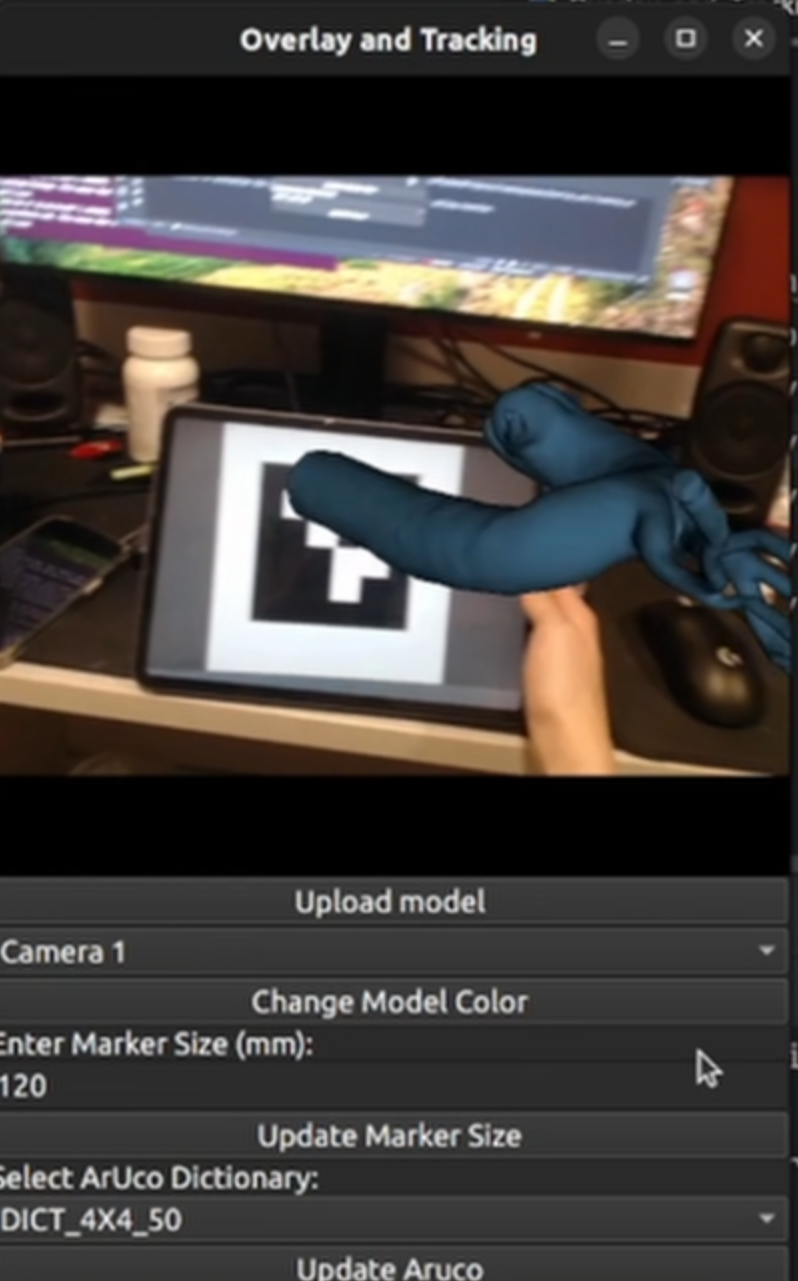
\includegraphics[width=0.6\textwidth]{tracking.png}
                              \caption{Overlay and Tracking}
                        \end{figure}
                  \item \textbf{Model Color change}
                        \\
                        In order to implement the model colour change functionality, it is necessary to reuse the model upload functionality mentioned in the \hyperref[sec:upload]{(a) Main Menu (Overlay and Tracking)} section. Before performing a model colour modification it will first check if a model exists in the VTK Overlay. If not, a warning box will be pushed to prompt the user to upload the model first. If the model is already loaded in VTK Overlay, when the model colour modification button is clicked in the Qt window, a colour picker dialog box will be opened in the Qt window allowing the user to select a colour. After the user selects a colour, a new model loader will be created and the model and colour will be reloaded using the model upload function mentioned in the \hyperref[sec:upload]{(a) Main Menu (Overlay and Tracking)} section. Once the model has been re-uploaded with the newly selected colours, update the VTK Render window to re-render the model Overlay to show the model with the modified colours.
                        \paragraph{Pseudocode Code for the Model Color change:}
                        \begin{minted}[frame=single, linenos=true, fontsize=\footnotesize]{python}
Method change_model_color:
    Check if the model directory has been loaded
    If no models are loaded:
        Display a warning dialog, "Please upload models first"
        Return

    Open a color picker dialog
    If a valid color is chosen:
        Convert the color to RGB format
        Create a model loader with the model directory and RGB color
        Add the loaded models to the VTK rendering window
        Re-render the window to update the color
                  \end{minted}
                        % 模型颜色修改截图展示
                        \begin{figure}[H]
                              \centering
                              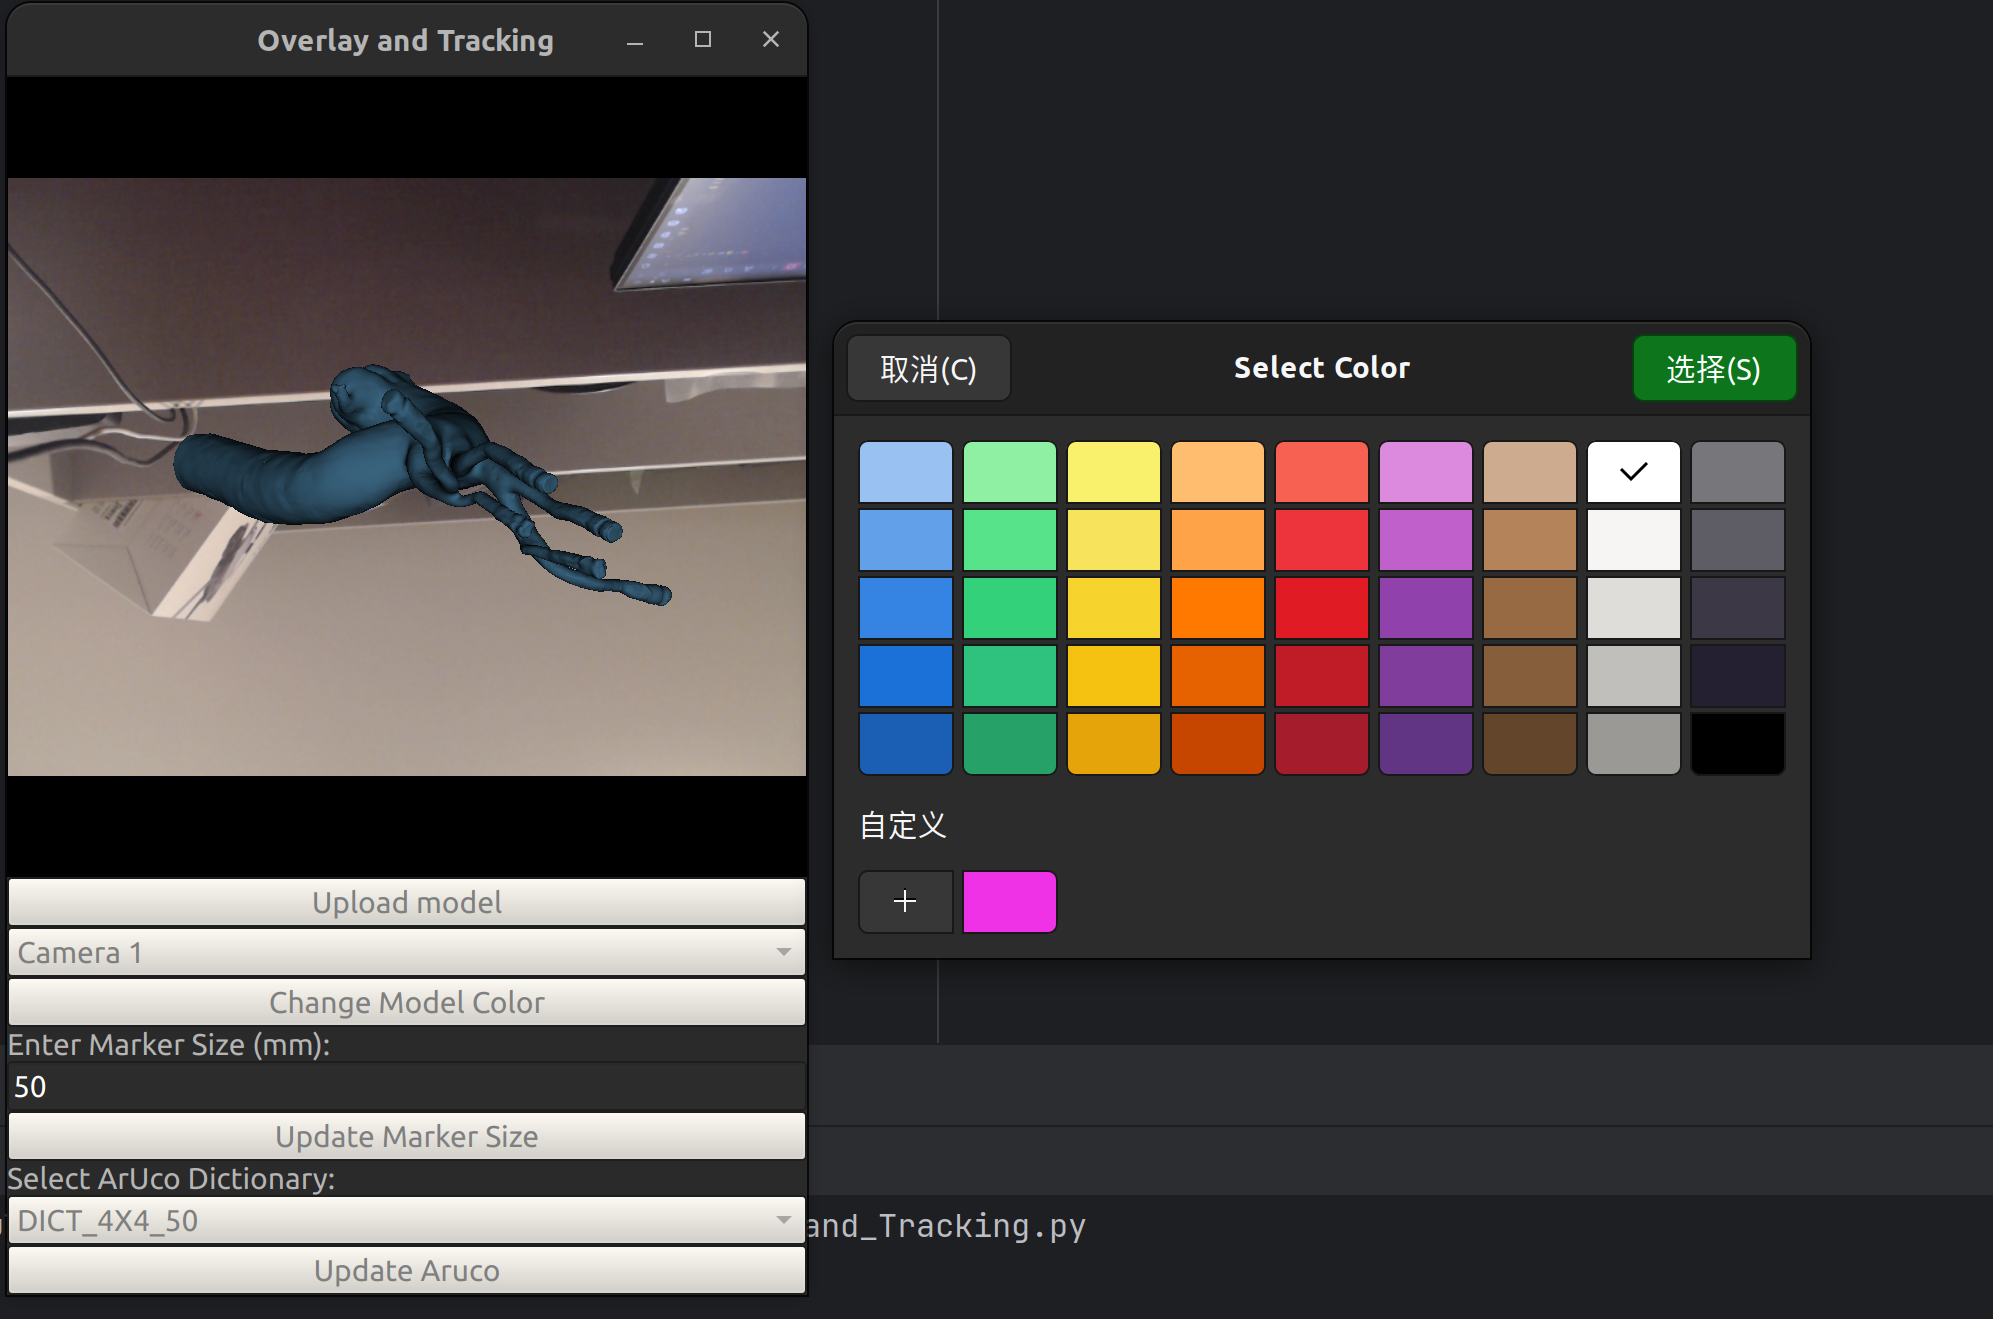
\includegraphics[width=0.6\textwidth]{coulor.png}
                              \caption{Colour Picker Dialog Box}
                        \end{figure}
                        \begin{figure}[H]
                              \centering
                              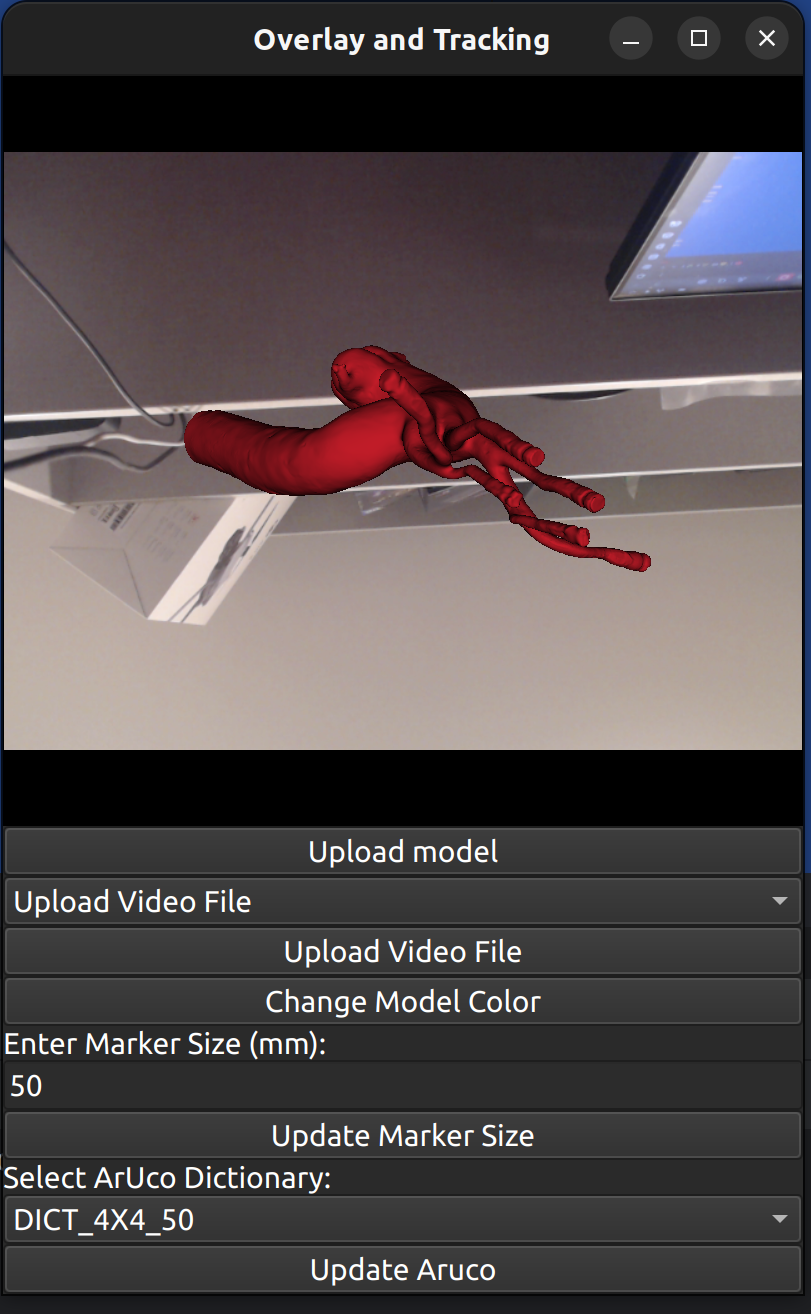
\includegraphics[width=0.3\textwidth]{upload.png}
                              \caption{Color Changed Model}
                        \end{figure}
                  \item \textbf{ArUco Marker Settings}
                        \\
                        The ArUco parameters are set up by setting up a text box for entering the size of the markers and a drop-down menu for selecting the ArUco lexicon.
                        \\\\
                        Firstly, a label and a text input box are created in the Qt window, allowing the user to enter the size of the ArUco markers (in millimetres) and update the settings with a button. After clicking on the "Update Marker Size" button, the system will read the size value entered by the user, update the settings, and then restart via the \hyperref[sec:tracking]{Start Tracking and Outputting Marker Pose Data} section. restarting the tracking thread to apply the new settings.
                        \\\\
                        Second, a drop-down menu was also created for the user to select the different ArUco dictionaries they use, as well as a button to update the selected dictionary. Once the user has selected a dictionary via the drop-down menu, clicking on the "Update ArUco" button triggers the update of the dictionary, which works in the same way as updating the tag size.
                        \paragraph{Pseudocode Code for the ArUco Marker Settings:}
                        \begin{minted}[frame=single, linenos=true, fontsize=\footnotesize]{python}
Method setup_marker_size_ui:
    Create label "Enter Marker Size (mm):"
    Add label to layout

    Create input field for marker size
    Set default text of input field to "50"
    Add input field to layout

    Create button "Update Marker Size"
    Connect button click event to method update_marker_size
    Add button to layout

Method update_marker_size:
    Read value from marker size input field
    Convert input value to float and store in marker size configuration
    Reinitialize ArUco tracker with updated configuration
    Start the ArUco tracker

Method setup_dictionary_ui:
    Create label "Select ArUco Dictionary:"
    Add label to layout

    Create dropdown for dictionary selection
    Populate dropdown with dictionary options:
        'DICT_4X4_50', 'DICT_4X4_100', etc.
    Add dropdown to layout

    Create button "Update Aruco"
    Connect button click event to method update_dictionary
    Add button to layout

Method update_dictionary:
    Get selected dictionary from dropdown
    Update ArUco dictionary in configuration with selected item
    Reinitialize ArUco tracker with updated configuration
    Start the ArUco tracker

                  \end{minted}
                        \begin{figure}[H]
                              \centering
                              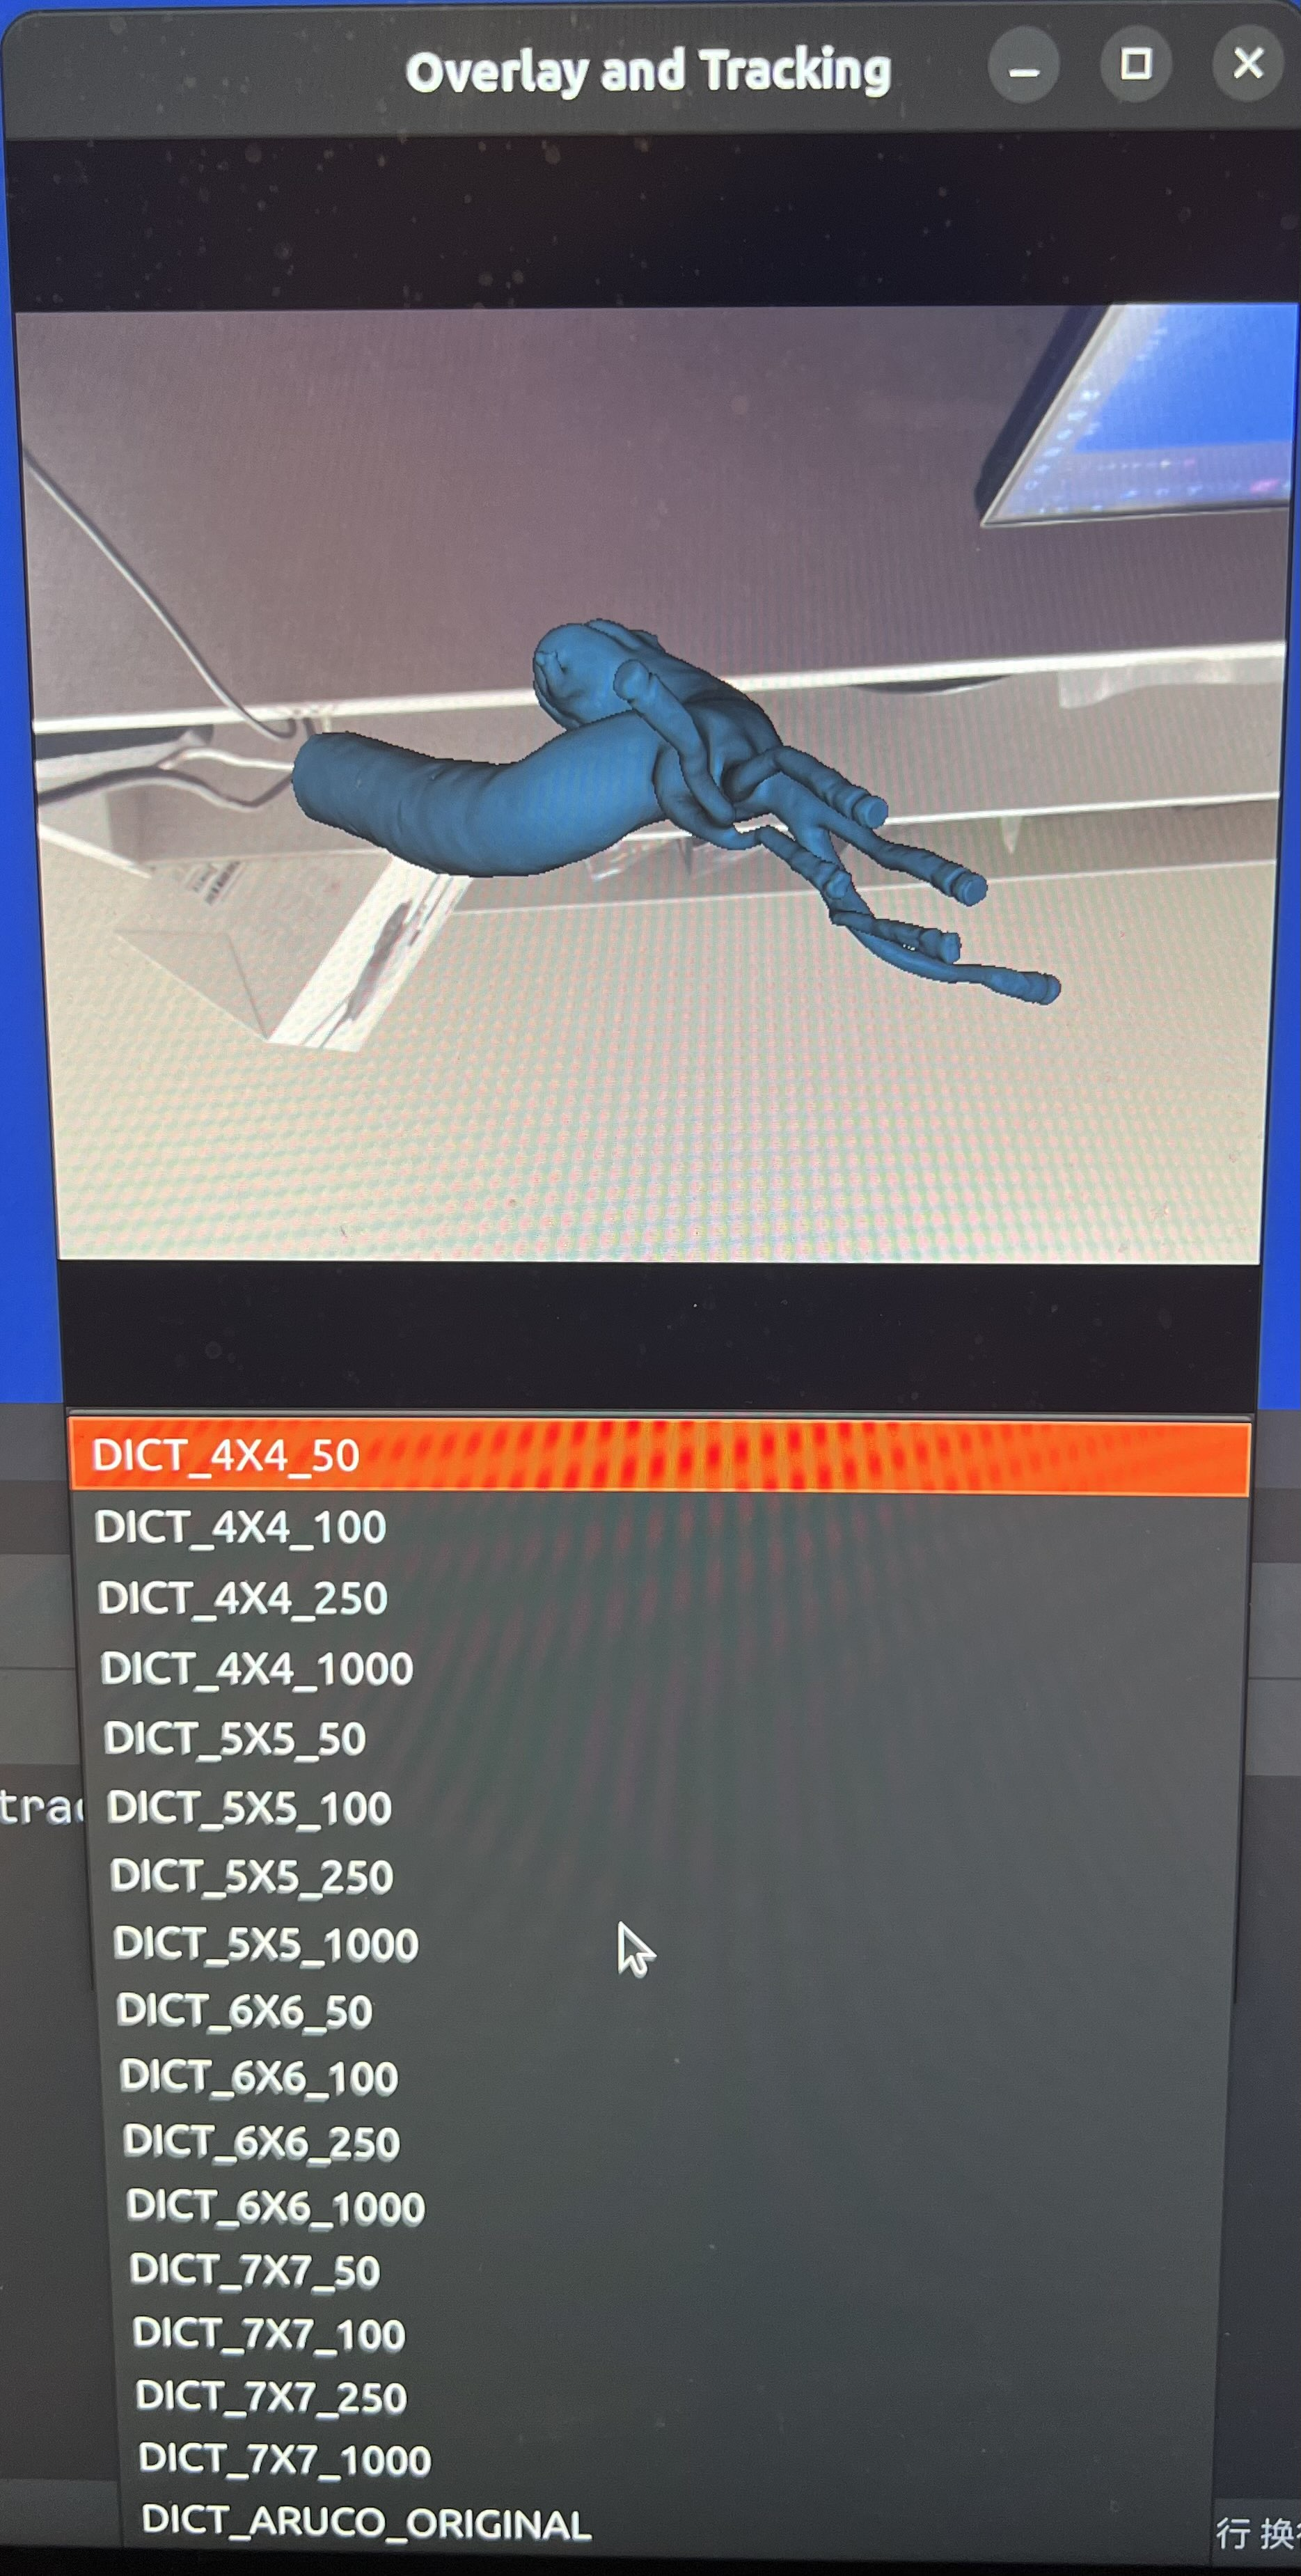
\includegraphics[width=0.3\textwidth]{select_aruco.jpg}
                              \caption{ArUco Dictionary Selection}
                        \end{figure}
                  \item \textbf{ArUco Generator}
                        \\
                        The ArUco Marker Generator application is the same as Overlay and Tacking, and is implemented by combining the ArUco module of OpenCV with a Qt graphical interface.
                        \\\\
                        The application first creates a user interface with a drop-down menu that allows the user to select from a variety of predefined ArUco dictionaries. After the user selects a dictionary, OpenCV's \emph{ aruco.getPredefinedDictionary} method is called to retrieve the corresponding dictionary, and then the \emph{aruco.drawMarker} method is used to generate markers of the corresponding size and dictionary. After that, the generated marker image is converted to QImage and QPixmap and displayed in the Qt interface.
                        \\\\
                        In addition, the ArUco marker saving function is also implemented, allowing the user to save the generated markers locally as an image file via the standard file dialogue box. When user clicks the "Save Marker" button, it will trigger the \emph{save\_marker} method. This method will open a file save dialogue box, allowing the user to select the file storage path and format. Upon user confirmation, the marker will be generated again using the current user-selected dictionary configuration to ensure that the latest generated image is saved, and the \emph{cv2.imwrite} method will be used to write the image to the specified folder with the default ArUco Dictionary filename.
                        \paragraph{Pseudocode Code for the ArUco Generator:}
                        \begin{minted}[frame=single, linenos=true, fontsize=\footnotesize]{java}
Class ArucoGenerator:
    Method __init__:
        Initialize GUI components
        Set initial ArUco dictionary to DICT_4X4_50
        Call init_ui to set up the user interface

    Method init_ui:
        Set window title to "ArUco Marker Generator"
        Create vertical layout for widgets

        Create dropdown for ArUco dictionary selection
        Add ArUco dictionary options to dropdown
        Connect dropdown change event to update_dictionary method
        Add dropdown to layout

        Create label to display marker image
        Add label to layout

        Create button "Save Marker"
        Connect button click event to save_marker method
        Add button to layout

        Generate initial marker

    Method update_dictionary:
        Read selected dictionary name from dropdown
        Update ArUco dictionary using selected name
        Generate new marker based on updated dictionary

    Method generate_marker:
        Get predefined dictionary using current ArUco dictionary setting
        Generate marker image for marker ID 0 with size 400x400 pixels
        Call show_marker with generated marker image

    Method show_marker(marker_image):
        Convert marker image to QImage with Grayscale format
        Convert QImage to QPixmap
        Set QPixmap on image label for display

    Method save_marker:
        Get current dictionary name from dropdown
        Set default filename based on selected dictionary and .png extension
        Open save file dialog with default filename and filter for PNG
        If file path is provided:
            Generate marker image again to ensure current settings are used
            Save marker image to file using OpenCV

Start Point:
    Initialize QApplication
    Create instance of ArucoGenerator
    Show window
    Execute QApplication
                        \end{minted}
                        \begin{figure}[H]
                              \centering
                              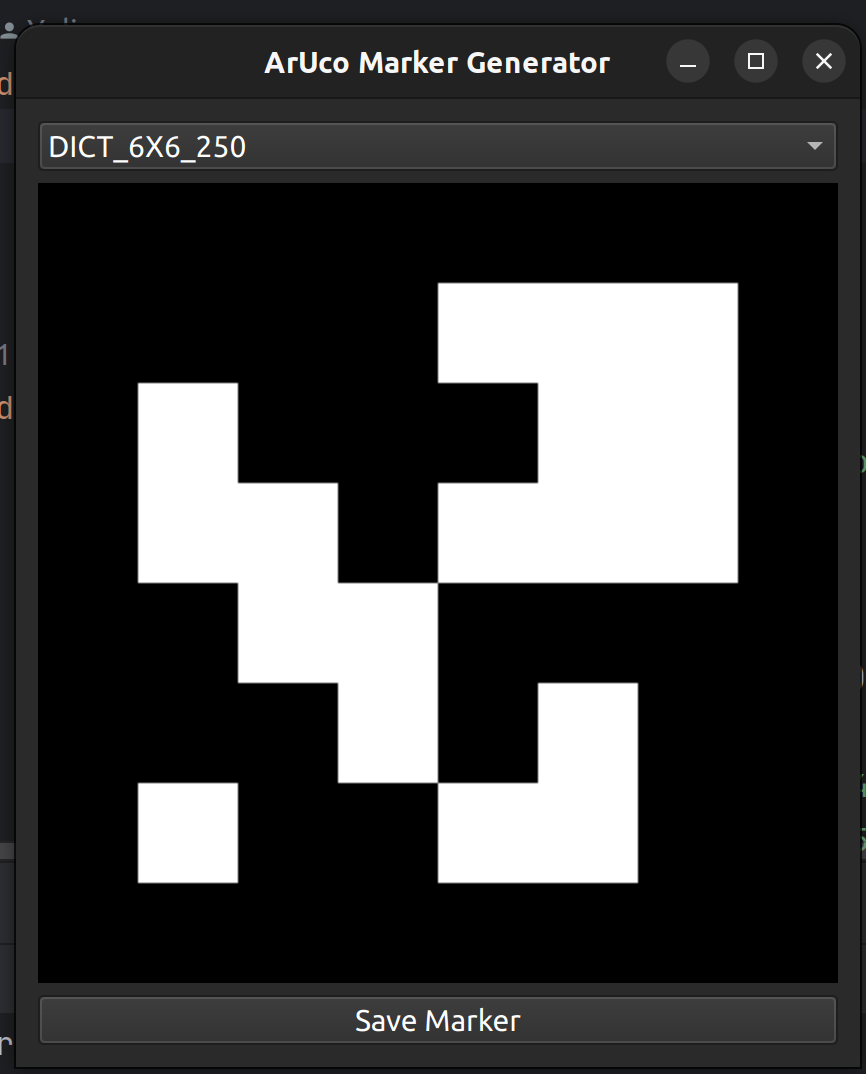
\includegraphics[width=0.4\textwidth]{change_aruco.png}
                              \caption{ArUco Generator Dictionary Changed}
                        \end{figure}
                        % ArUco 保存
                        \begin{figure}[H]
                              \centering
                              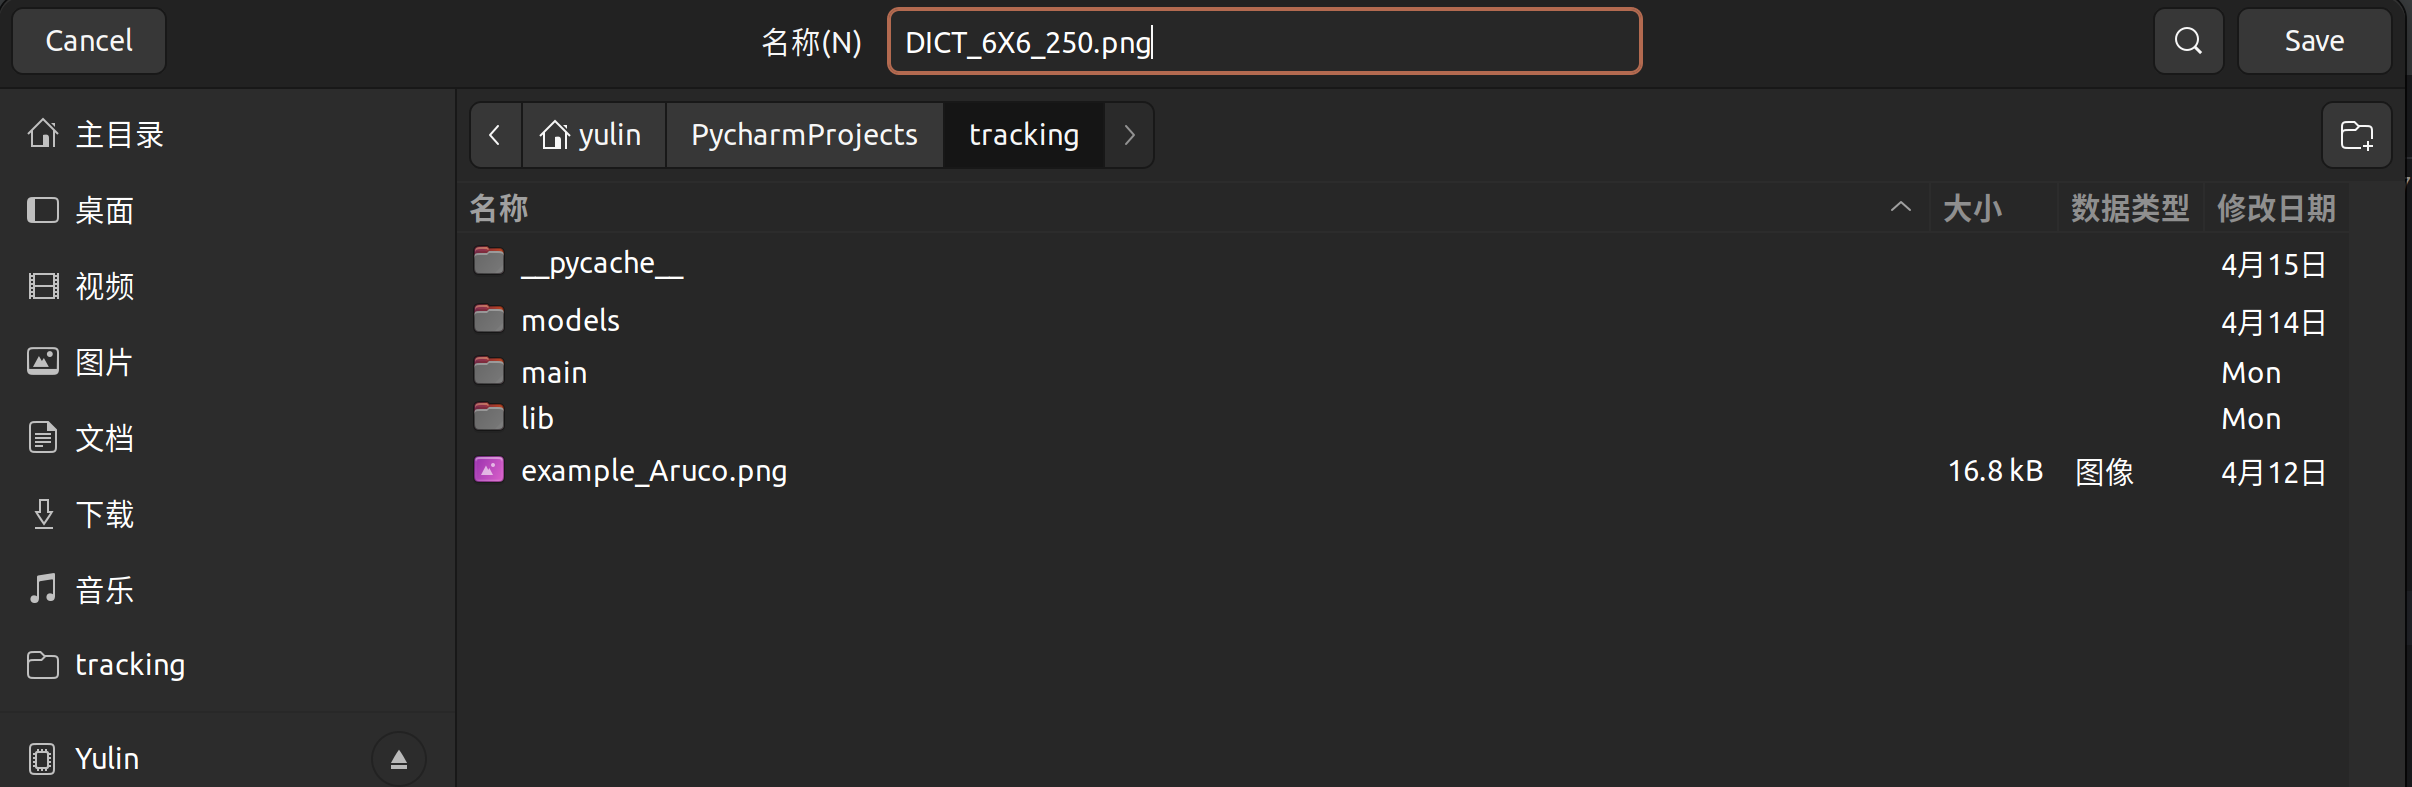
\includegraphics[width=1.2\textwidth]{save.png}
                              \caption{ArUco Marker Saved}
                        \end{figure}
            \end{enumerate}
      \item \textbf{Frontend Implementation}
      \\
      In this project, the front-end Qt interface is implemented through the \gls{pyside} framework. The various controls on the interface are organised by creating a vertical layout manager, QVBoxLayout. The margins and spacing of the layout were set to zero for the sake of indirection and to maximise space usage.
      \\\\
      The interface includes several features and key components that have been implemented in the previous section \hyperref[sec:backend]{Backend Implementation}: a drop-down menu that allows the user to select different video sources, a video upload button, an upload button that enables the user to upload a 3D model file, a colour selection button to adjust the display colour of the model, a text box to set the size of the actual ArUco icon and a drop-down menu for selecting the ArUco dictionary.
      \\\\
      These components are connected to the appropriate functional functions through signalling and slotting mechanisms to ensure that user actions trigger the appropriate response\cite{lazar2018mastering}. For example, the selection of a video source is done via a drop-down menu, and a function is called to update the video source used by the system when the selection is changed. Similarly, the colour change of a model is done by opening the colour dialog, and when the user selects a new colour, the system applies this colour to the 3D model.
      \\\\
      In addition, a VTK display window is integrated to display the video stream and the 3D model, which is adapted to the user's operating system to ensure compatibility. Due to the high extensibility of the Qt interface, new components and features can be easily added to the interface in the future.
      
            \paragraph{Code for the Frontend Implementation:}
            \begin{minted}[frame=single, linenos=true, fontsize=\footnotesize]{python}
class QtWidget(QWidget):
    def __init__(self, video_source, dims=None):
        super().__init__()
        # Setup the layout for the widget
        self.color_button = None
        self.layout = QVBoxLayout(self)
        self.layout.setContentsMargins(0, 0, 0, 0)
        self.layout.setSpacing(0)

        # Initialize the VTK overlay window, conditionally based on the OS
        init_vtk_widget = platform.system() != 'Linux'
        self.vtk_overlay_window = 
        VTKOverlayWindow(offscreen=False, init_widget=init_vtk_widget)
        self.layout.addWidget(self.vtk_overlay_window)

        # Initialize the video source
        self.video_source = TimestampedVideoSource(video_source, dims)

        # Set up a timer to update the view periodically
        self.timer = QTimer()
        self.timer.timeout.connect(self.update_view)
        self.update_rate = 30
        self.model_dir = None
        # Setup additional controls
        self.setup_upload_button()
        self.setup_video_source_controls()
        self.setup_color_change_button()
            \end{minted}
\end{enumerate}

\subsection{Part2: Endovascular Intervention Simulation}
% 在这里详细介绍关于“Endovascular Intervention Simulation”的设计和实现。
Our project combines machine learning with AR/VR \cite{9376657,Ranne2023AiAReSegCD} to create an open-source simulator for autonomous cannulation in endovascular operations. This project try to offer a high-fidelity model of the catheter
and aorta, integrating an advanced endovascular robot. It is designed to provide real-time force sensing and has shown, through prelimi-
nary tests, to effectively mimic real-world robot behaviours\cite{jianu2022cathsim}. Furthermore, we aim to deploy CathSim on VR devices like
HoloLens or Meta Quest\cite{Quest}, enhancing its accessibility and utility for medical professionals.
\subsubsection{Design}
% 描述“Endovascular Intervention Simulation”部分的设计细节。
\begin{enumerate}
      \item \textbf{Rope Design}
      \label{sec:rope}
      \\
      Early in the design process, I considered two different approaches to Rope design and did an initial practice and comparison of them.
      \\\\
      Firstly, I used a Rope constructed from a slender cylinder cut into multiple sub-cylinders, each of which is equivalent to a node of a rope, and used Unity C\# scripts to control each node to enable the bending and elongation of the rope and to try and make this rope give feedback on the forces exerted by the outside world.
      \begin{figure}[H]
            \centering
            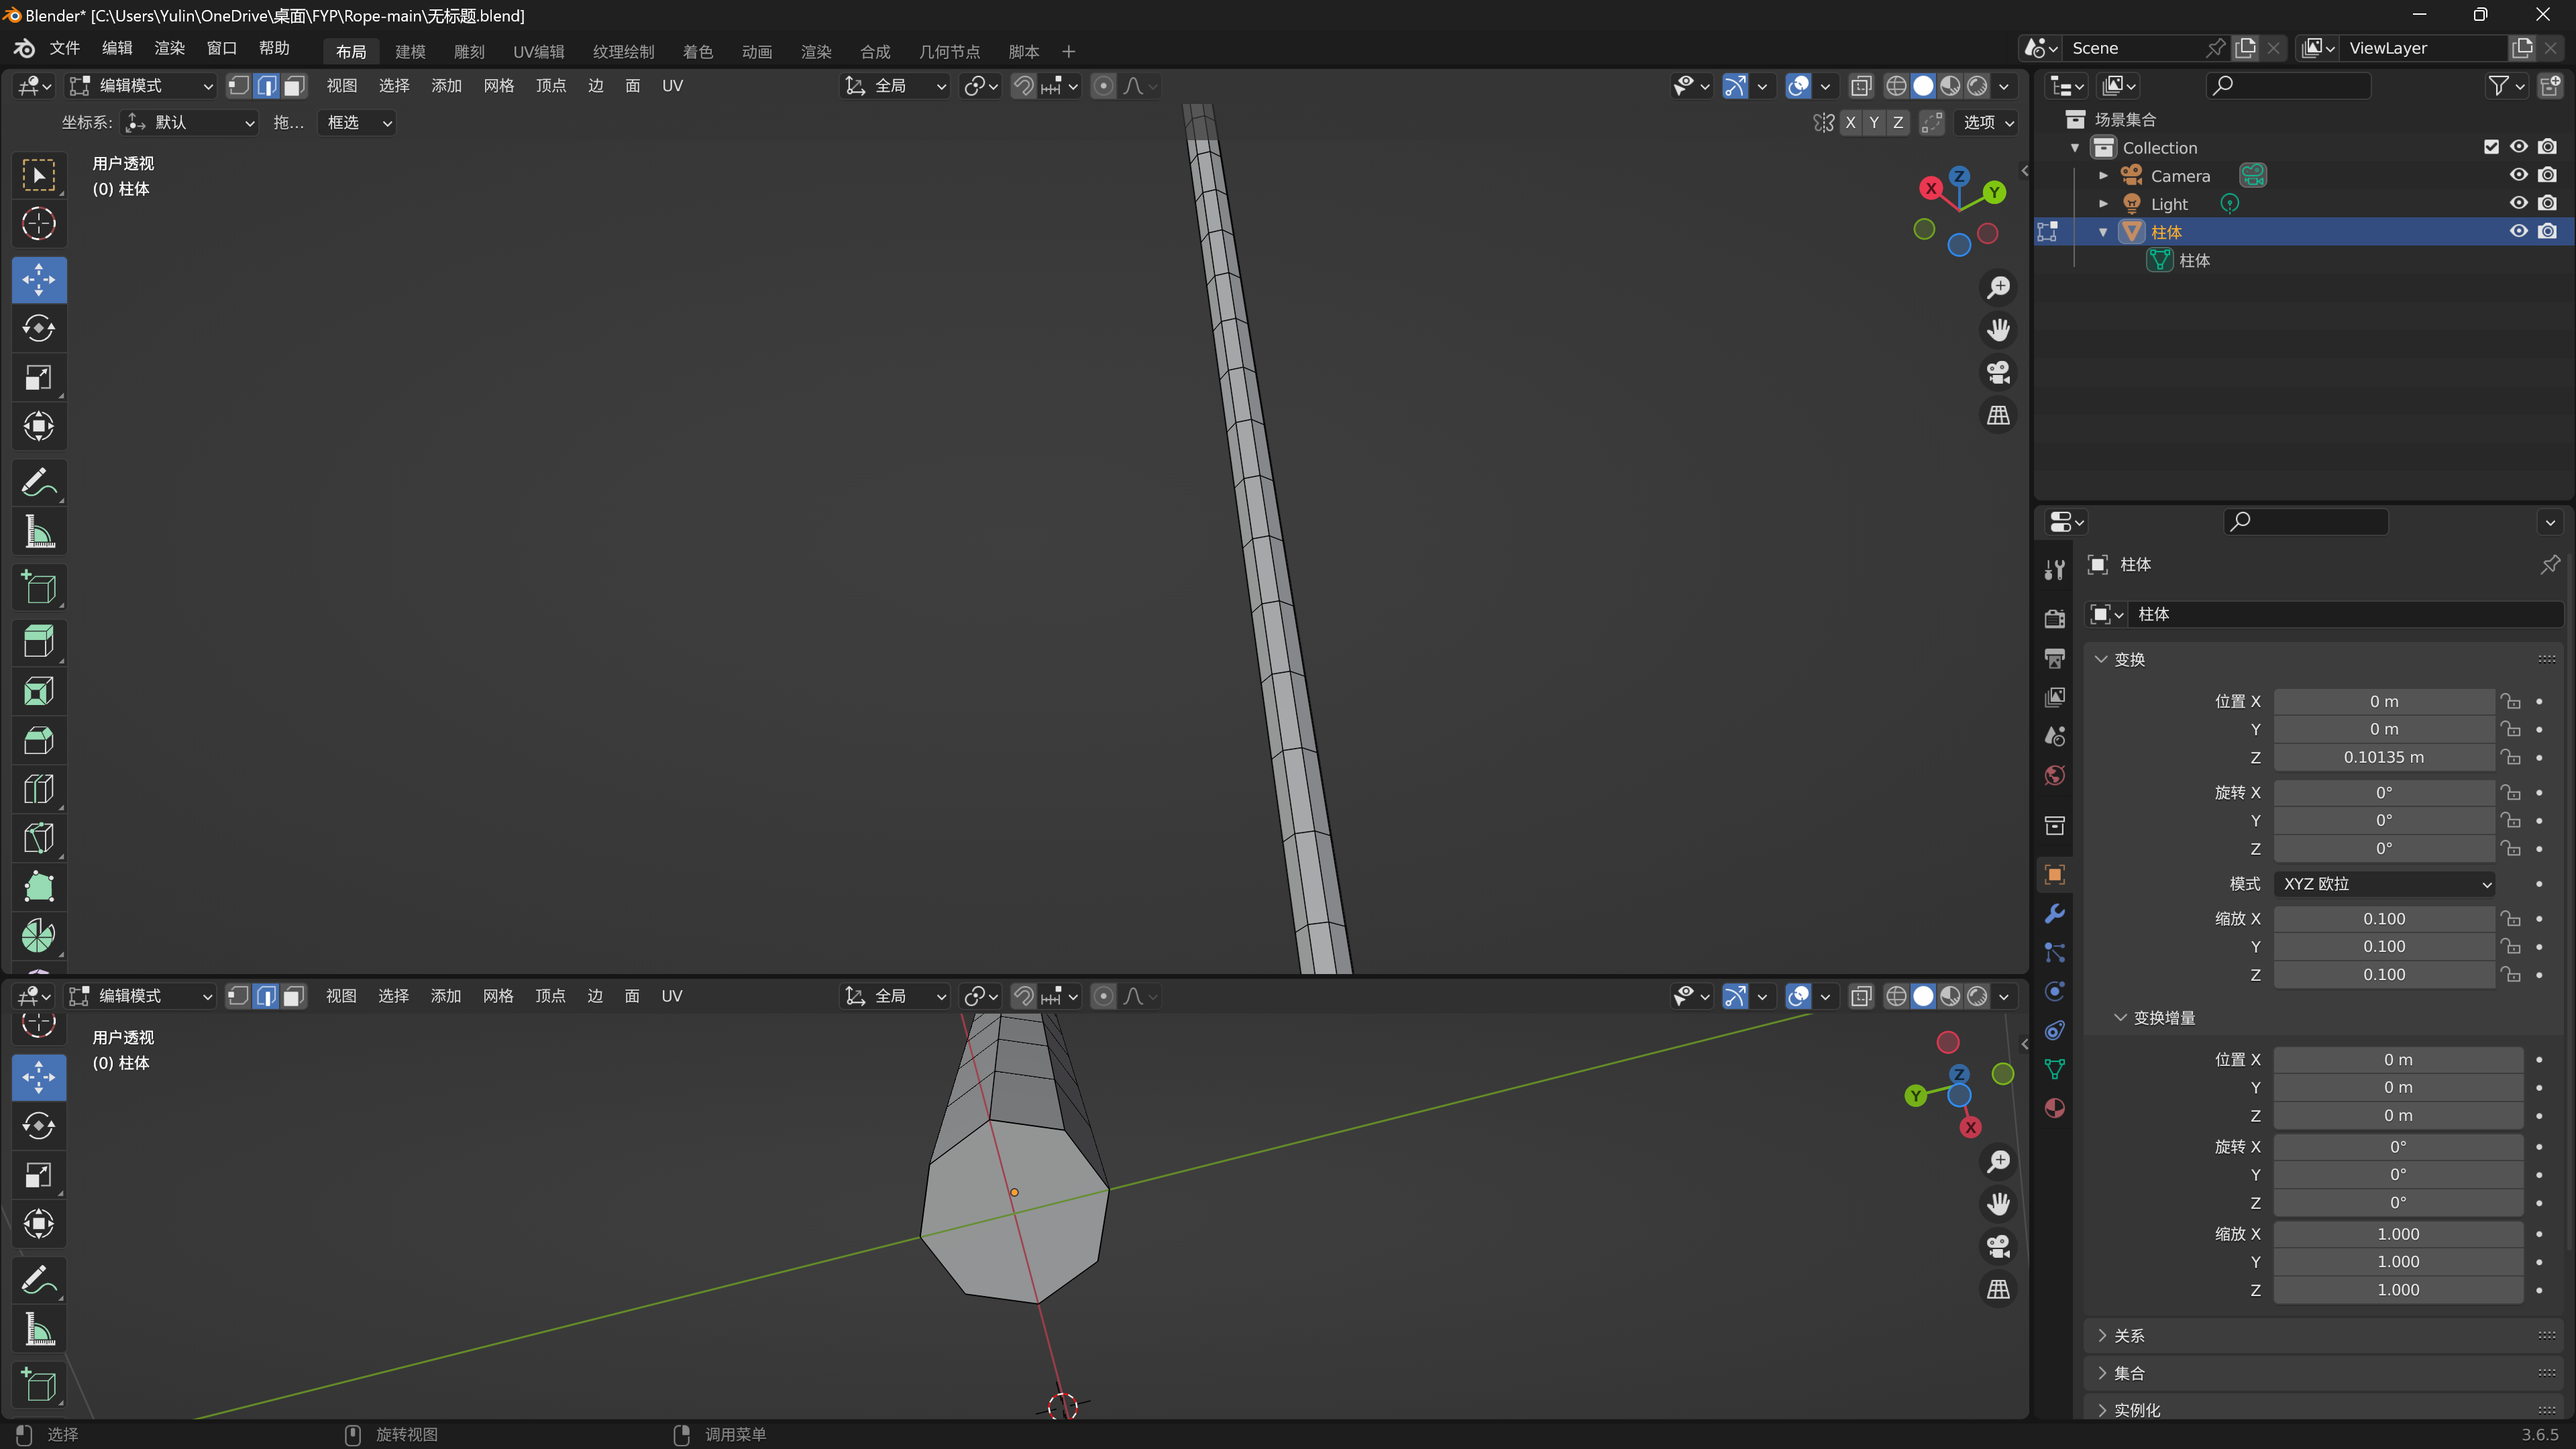
\includegraphics[width=0.8\textwidth]{blender design.png}
            \caption{Rope Design in Blender}
      \end{figure}
      In the second approach, I attempted to splice multiple identical and separate cubes into a Rope using Unity C\# scripting directly. The bending and stretching of the rope was achieved by controlling each cube and their gaps directly through the script.
      \begin{figure}[H]
            \centering
            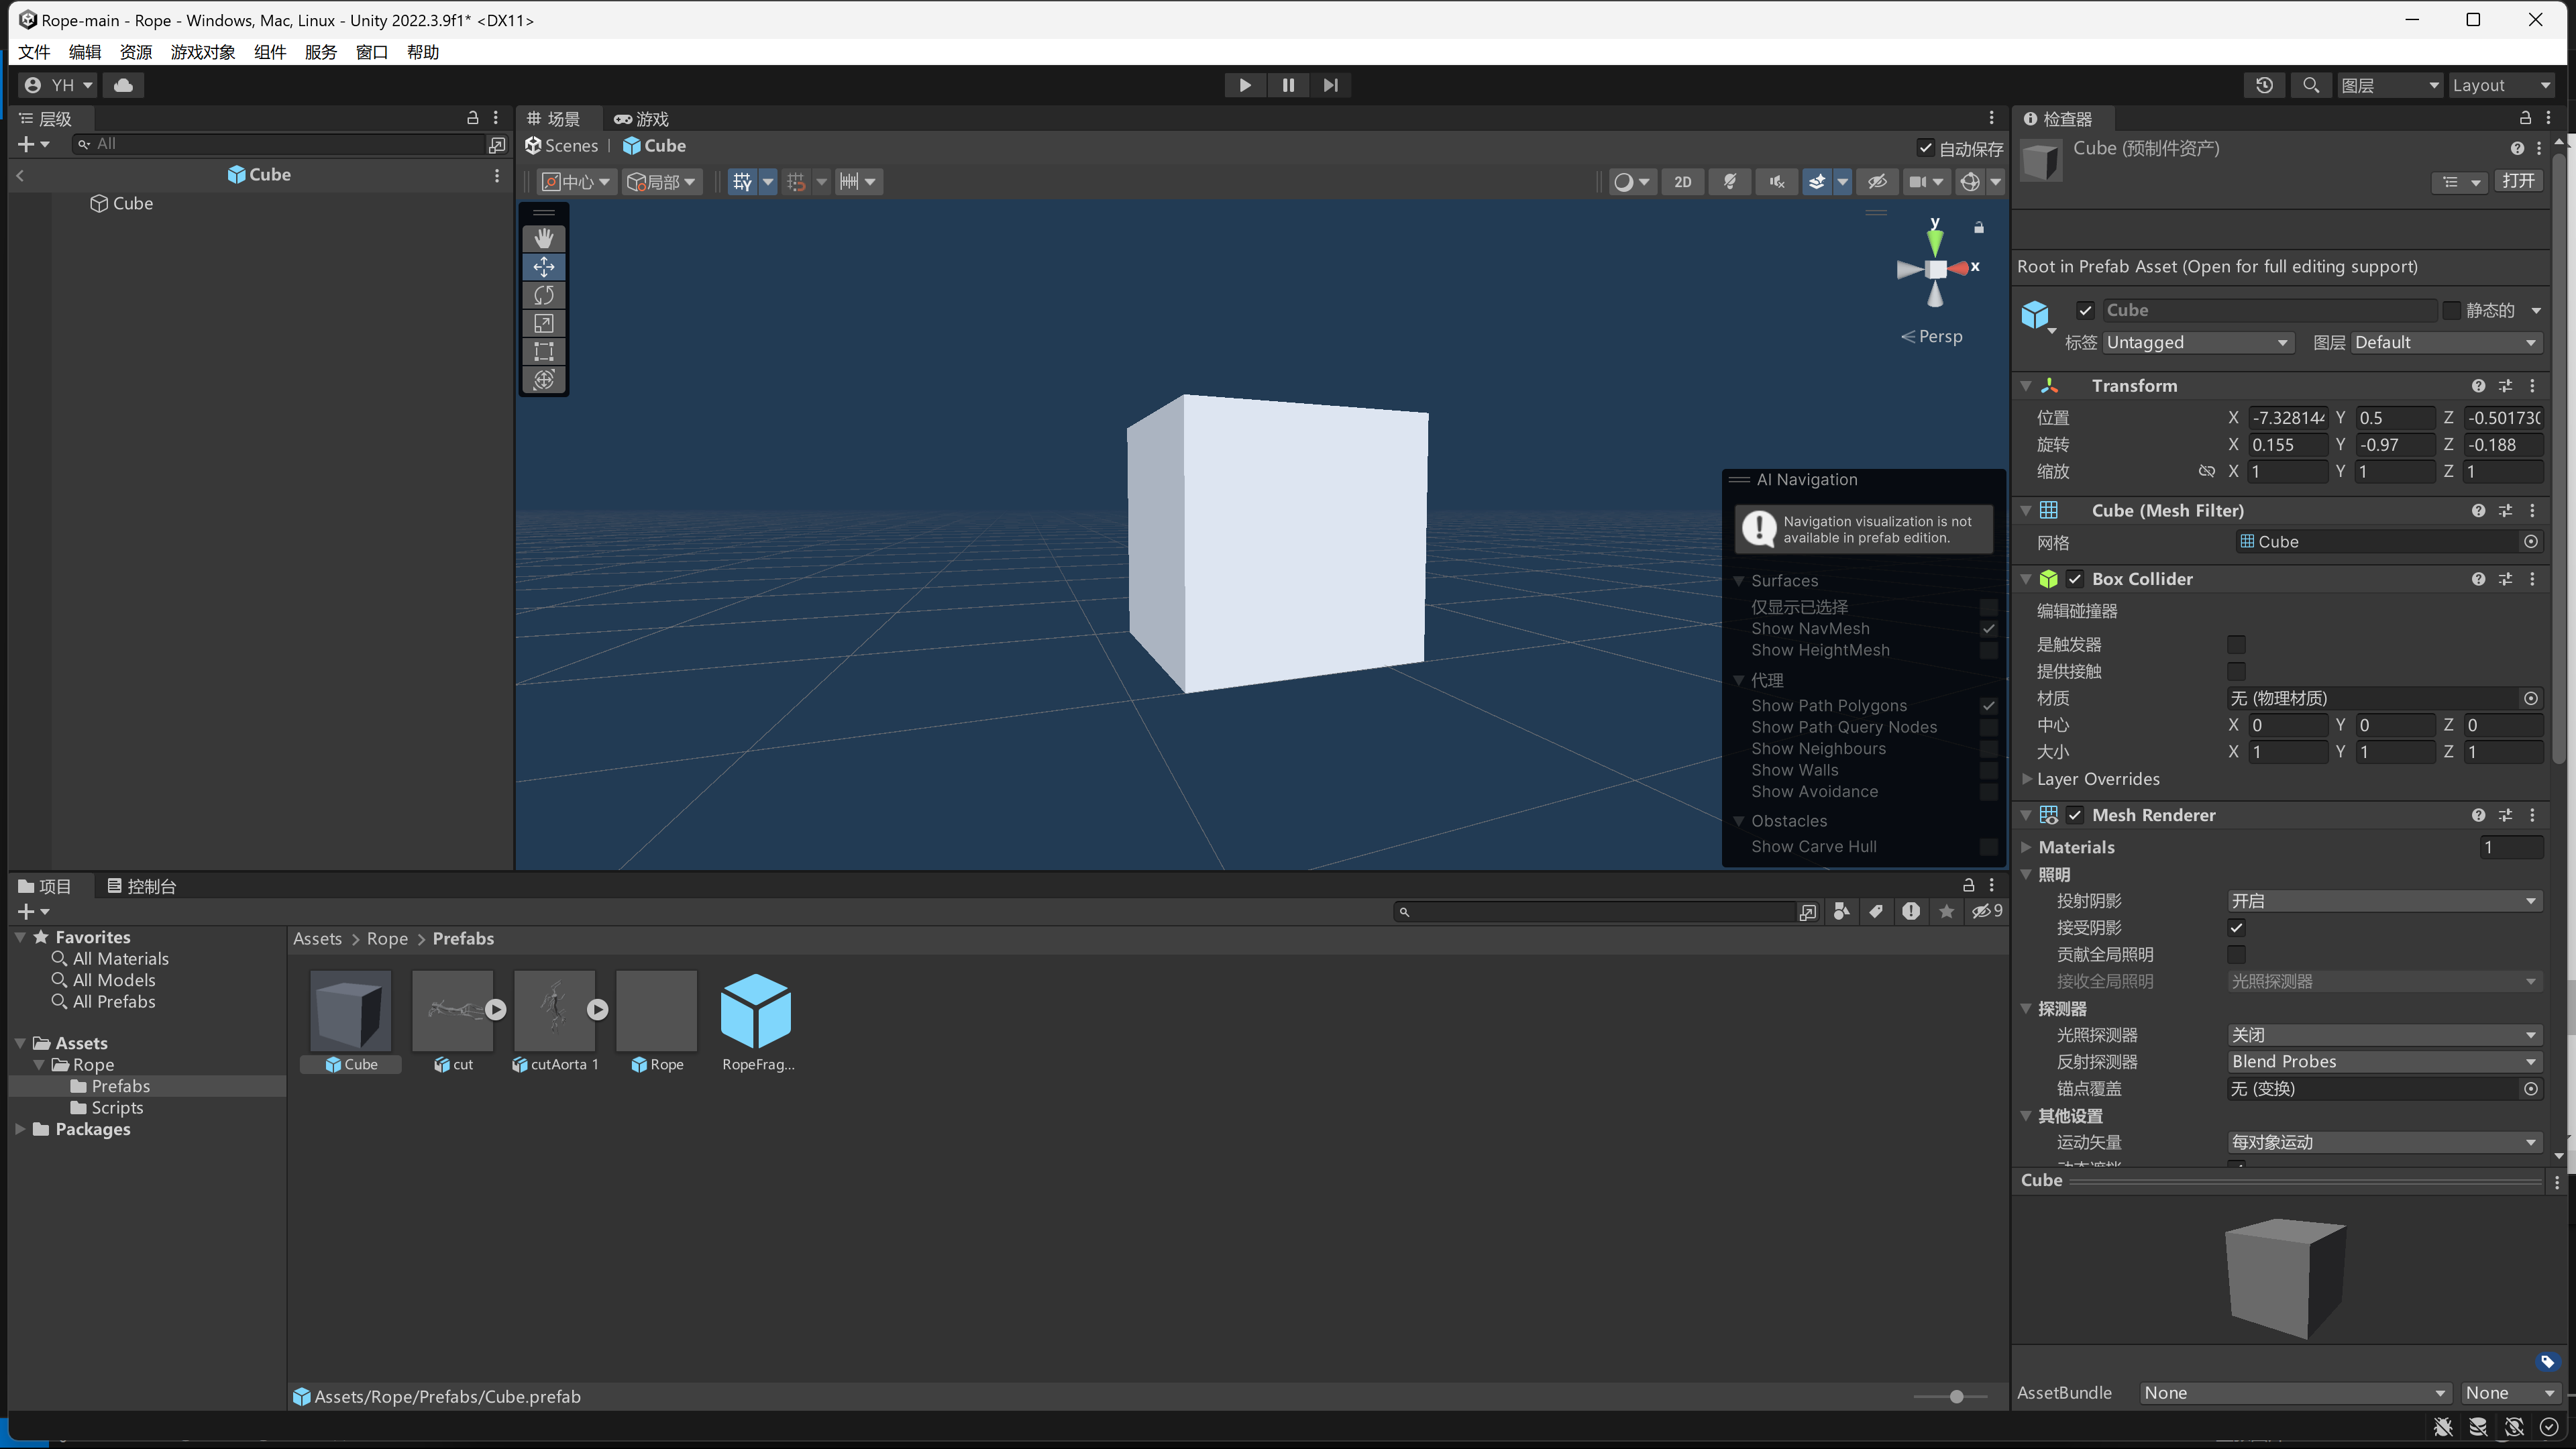
\includegraphics[width=0.8\textwidth]{cube.png}
            \caption{Cube Fragement}
      \end{figure}
      Either way, there were a lot of serious and difficult to locate and solve problems in the early stages of the project, and both implementations had major flaws and loopholes.

      \item \textbf{Model Design}
      \\
      The model used for this project was derived from a distribution made by Supervisor at the beginning of the project, with all members using the same Aorta model. In addition to the Aorta model, we have the Catheter model and the Catheter controller model.
      \\\\
      In order for Rope to have access to the Aorta model, the Aorta model needs to be modified using Blender. By optimising the number of triangles that the Aorta has, and by cutting and opening up the ends of the blood vessels in the Aorta model, the Rope can be inserted into the Aorta model without any problems.
      \begin{figure}[H]
            \centering
            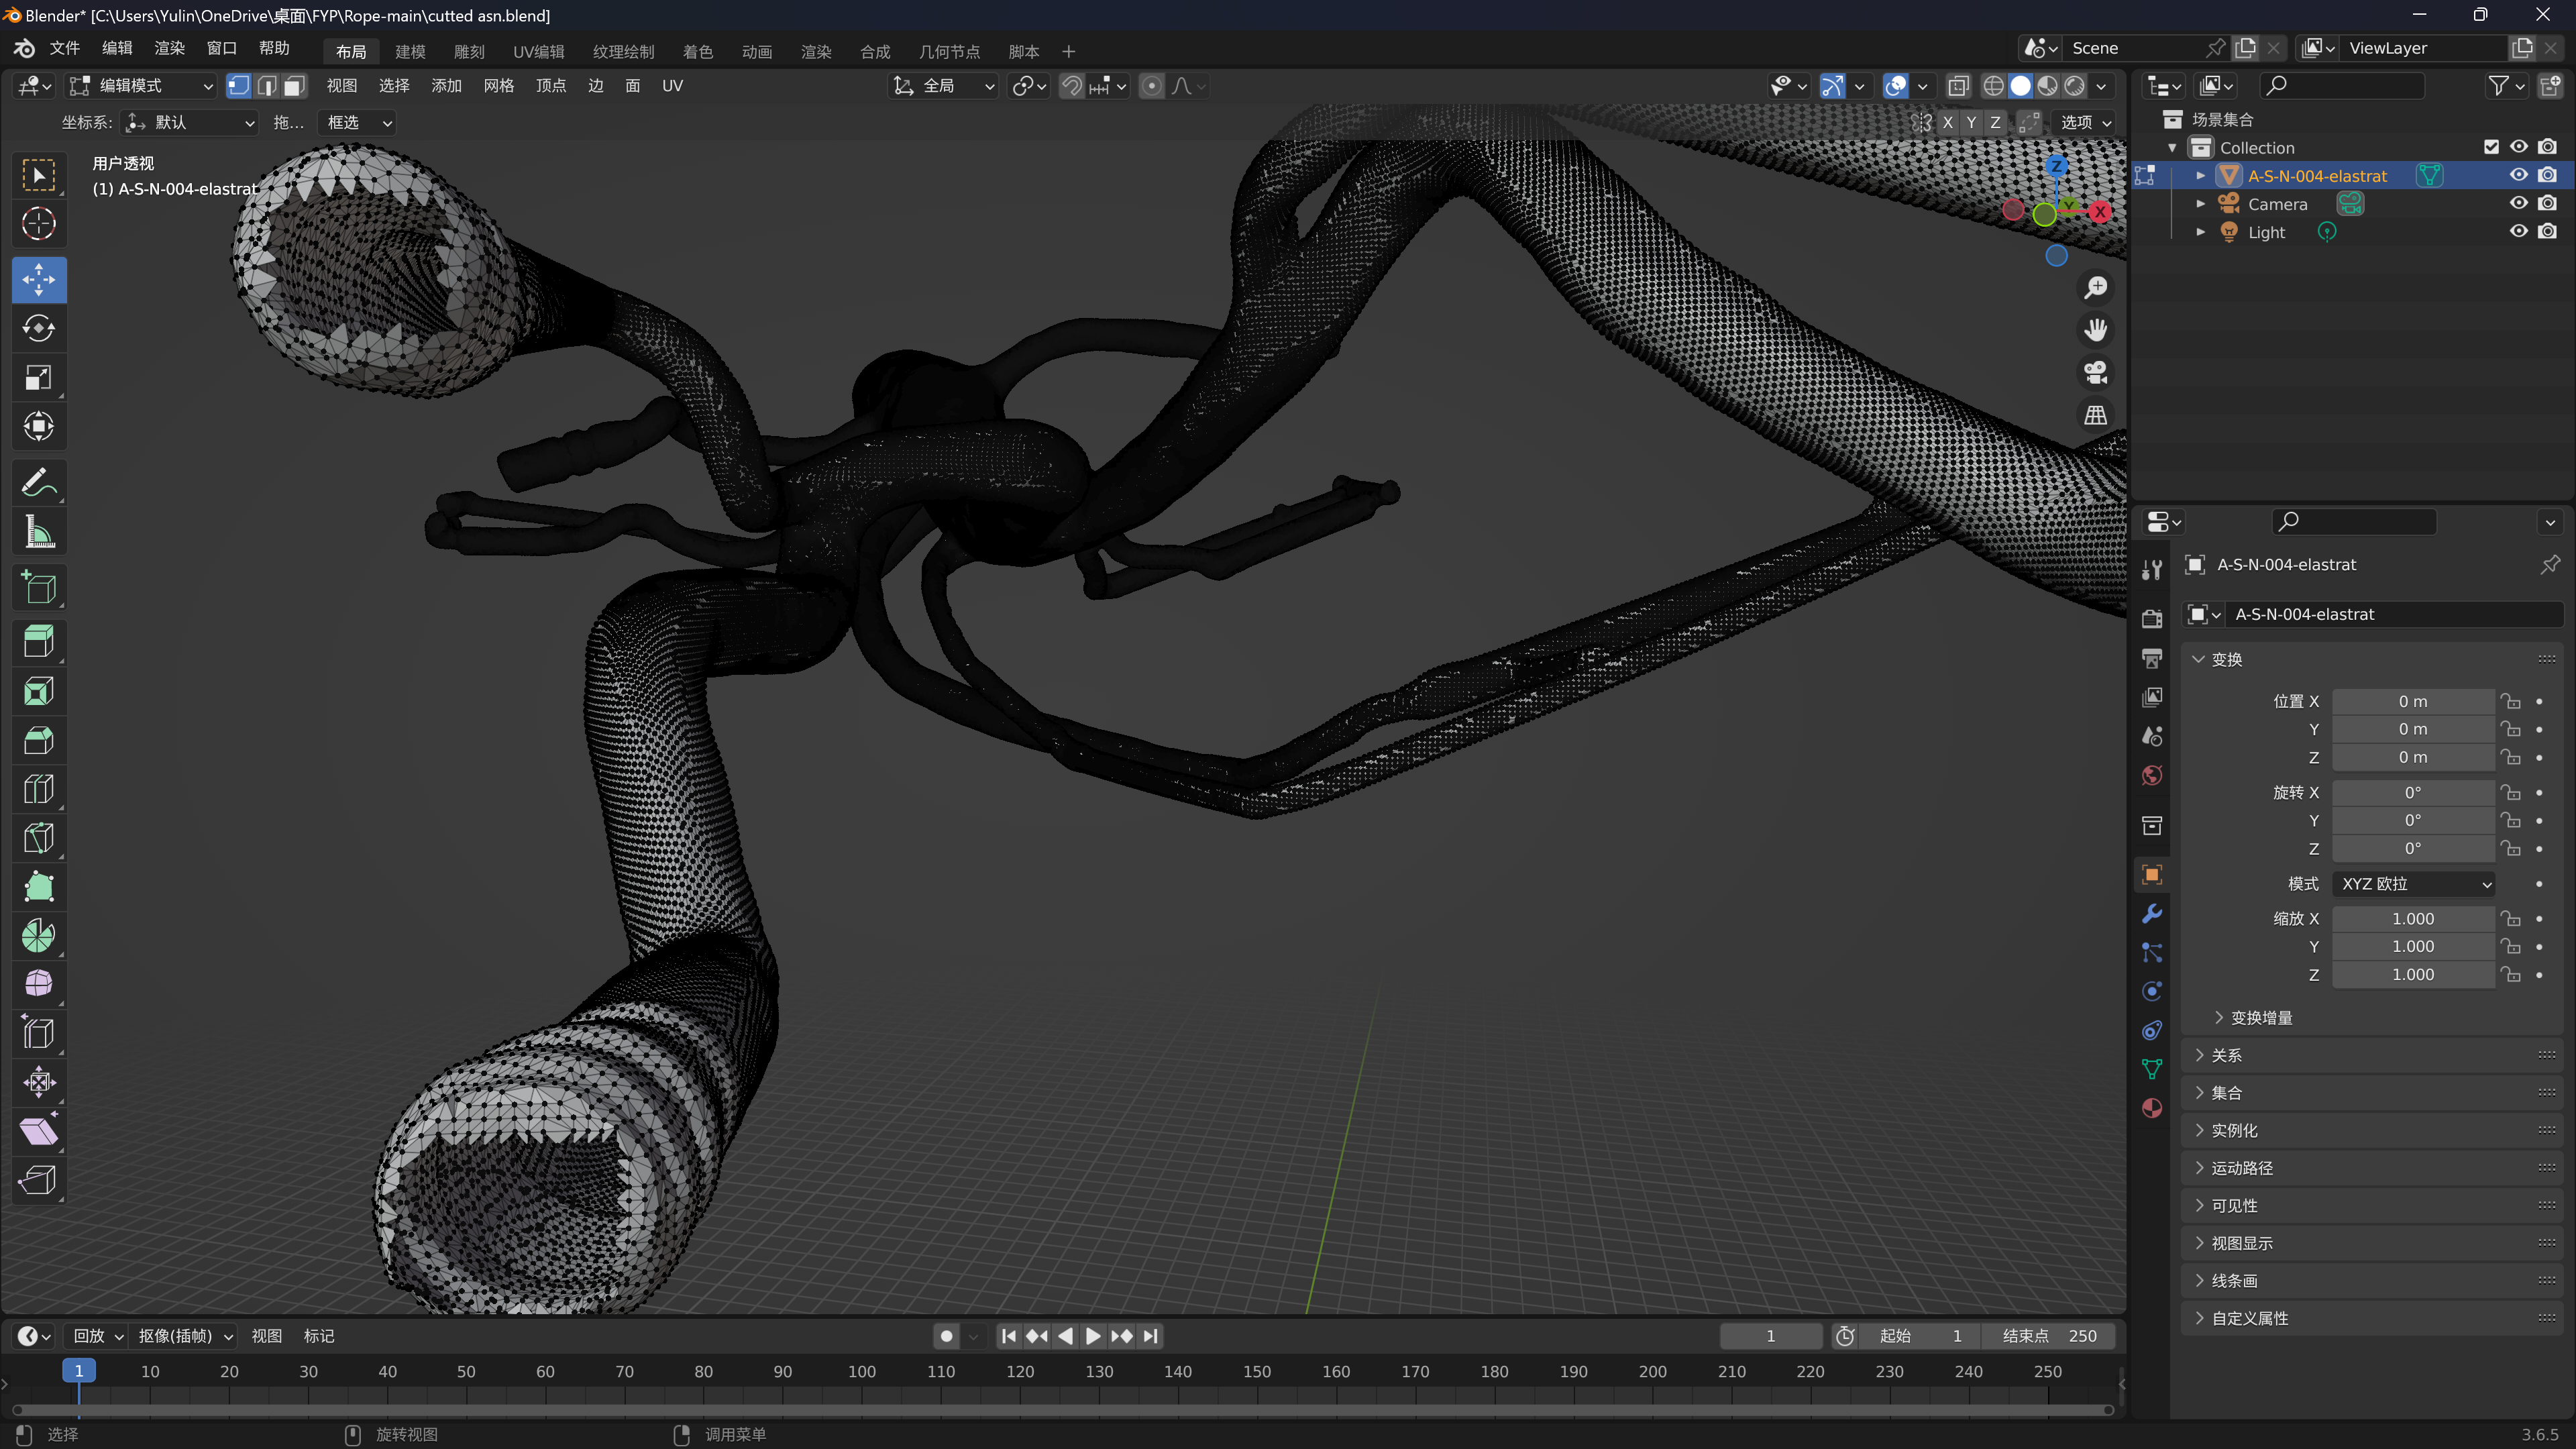
\includegraphics[width=0.8\textwidth]{blender cut.png}
            \caption{Cut Aorta Model}
      \end{figure}
      \item \textbf{Endovascular Intervention Simulation Design}
      \\
      Endovascular Intervention Simulation is the core part of Part2. It was planned to control the Rope and Catheter in some way, including movements such as rotation, forward, backward and bending. This would allow the Rope to enter the Aorta model and move under the control of the user, with force feedback (e.g. bending, etc.) when it touches the walls of the Aorta. When touching the Aorta wall it should also follow the path of the Aorta deeper under the control of the user, in which case the Rope should bend with the curve of the inner wall of the Aorta and remain inside the Aorta model without escaping.
      \\\\
      In the original design, it was planned to use a slider to control the forward and backward motion movement of Rope and Catheter. However, this control method has serious flaws, Rope can only move back and forth but not bend and rotate under the control of this method. So this control method was abandoned at the early stage of design.
      \begin{figure}[H]
            \centering
            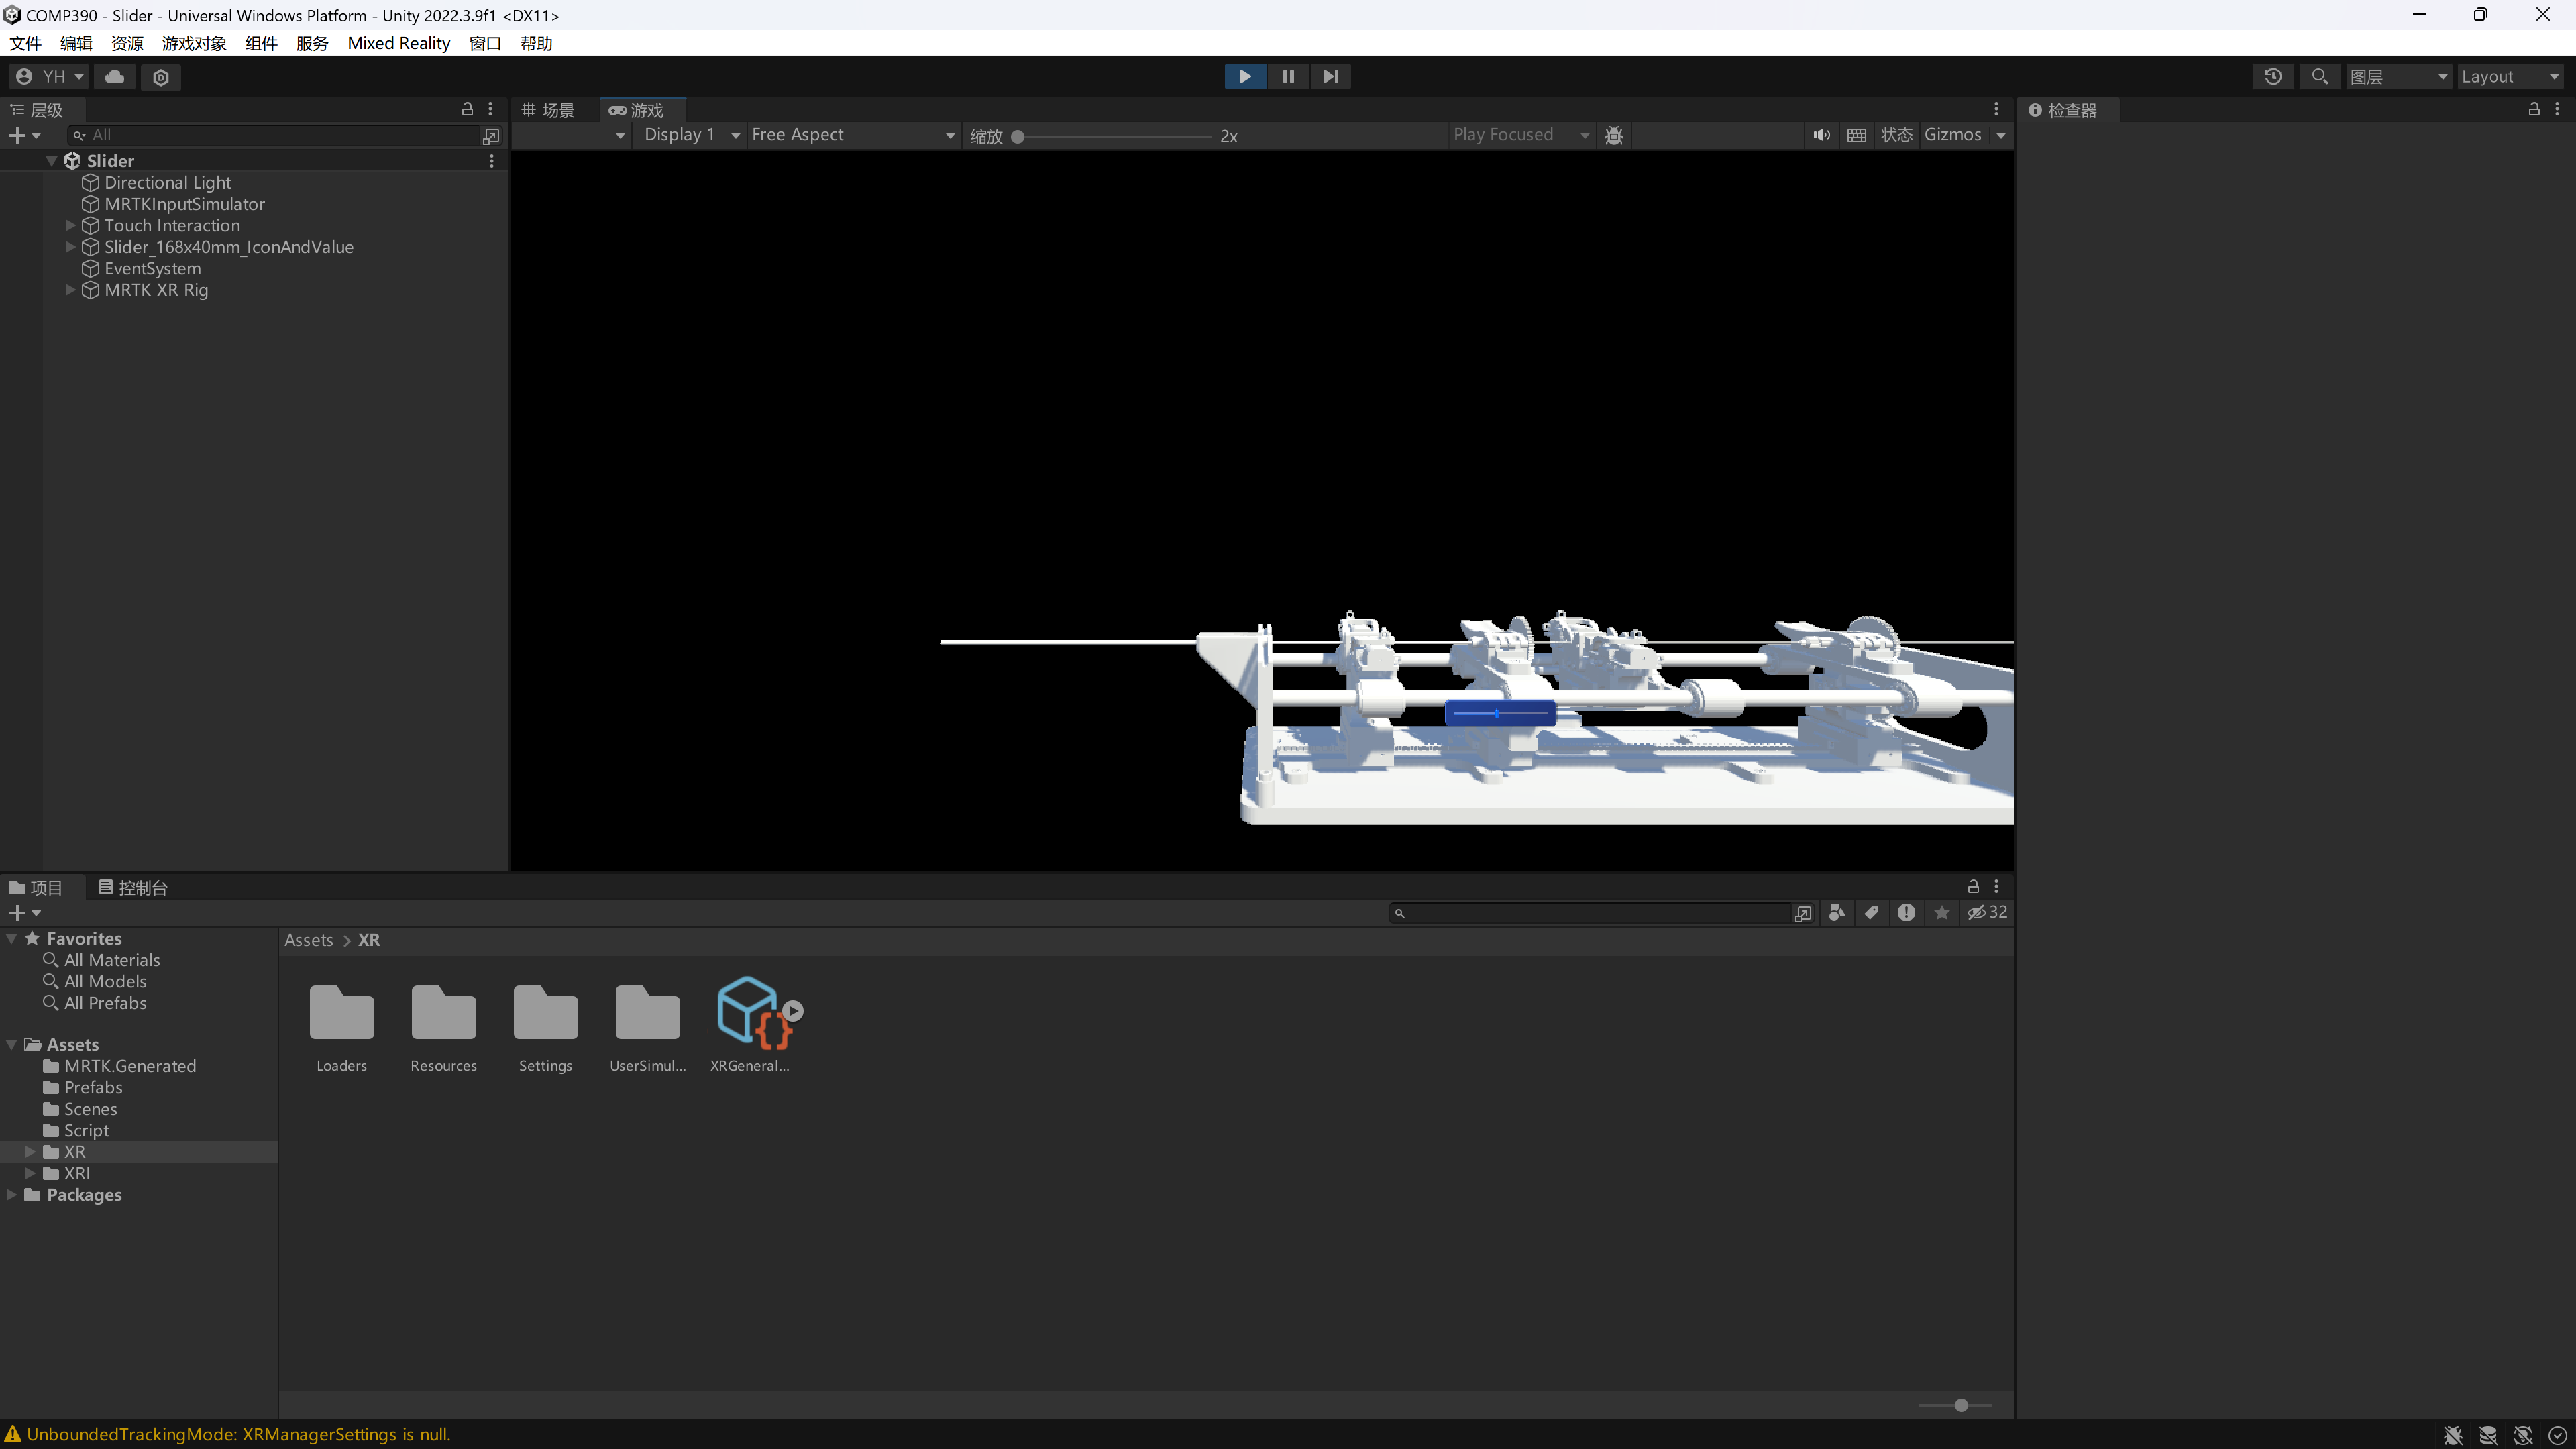
\includegraphics[width=0.8\textwidth]{slider.png}
            \caption{Slider Control Design}
      \end{figure}
      After that, we tried to use a cylinder to control Rope under the suggestion of Supervisor. Compared with the slider, the cylinder can control the Rope's forward, backward and rotation at the same time. However, since we are conducting the development of AR/VR project and the ultimate goal is to deploy it on AR/VR related devices, using a cylinder may not be convenient for users to operate it while using virtual reality devices. The design and implementation was previously discarded.
      \\\\
      In the end, we chose to use \gls{mrtk} for development. This development framework can provide a simulated palm for direct control of the Rope. Simulated finger pinching can be performed through the handle of the VR/AR device. Thus, the Rope can be simultaneously controlled with forward and backward motion, rotation and bending.
      \begin{figure}[H]
            \centering
            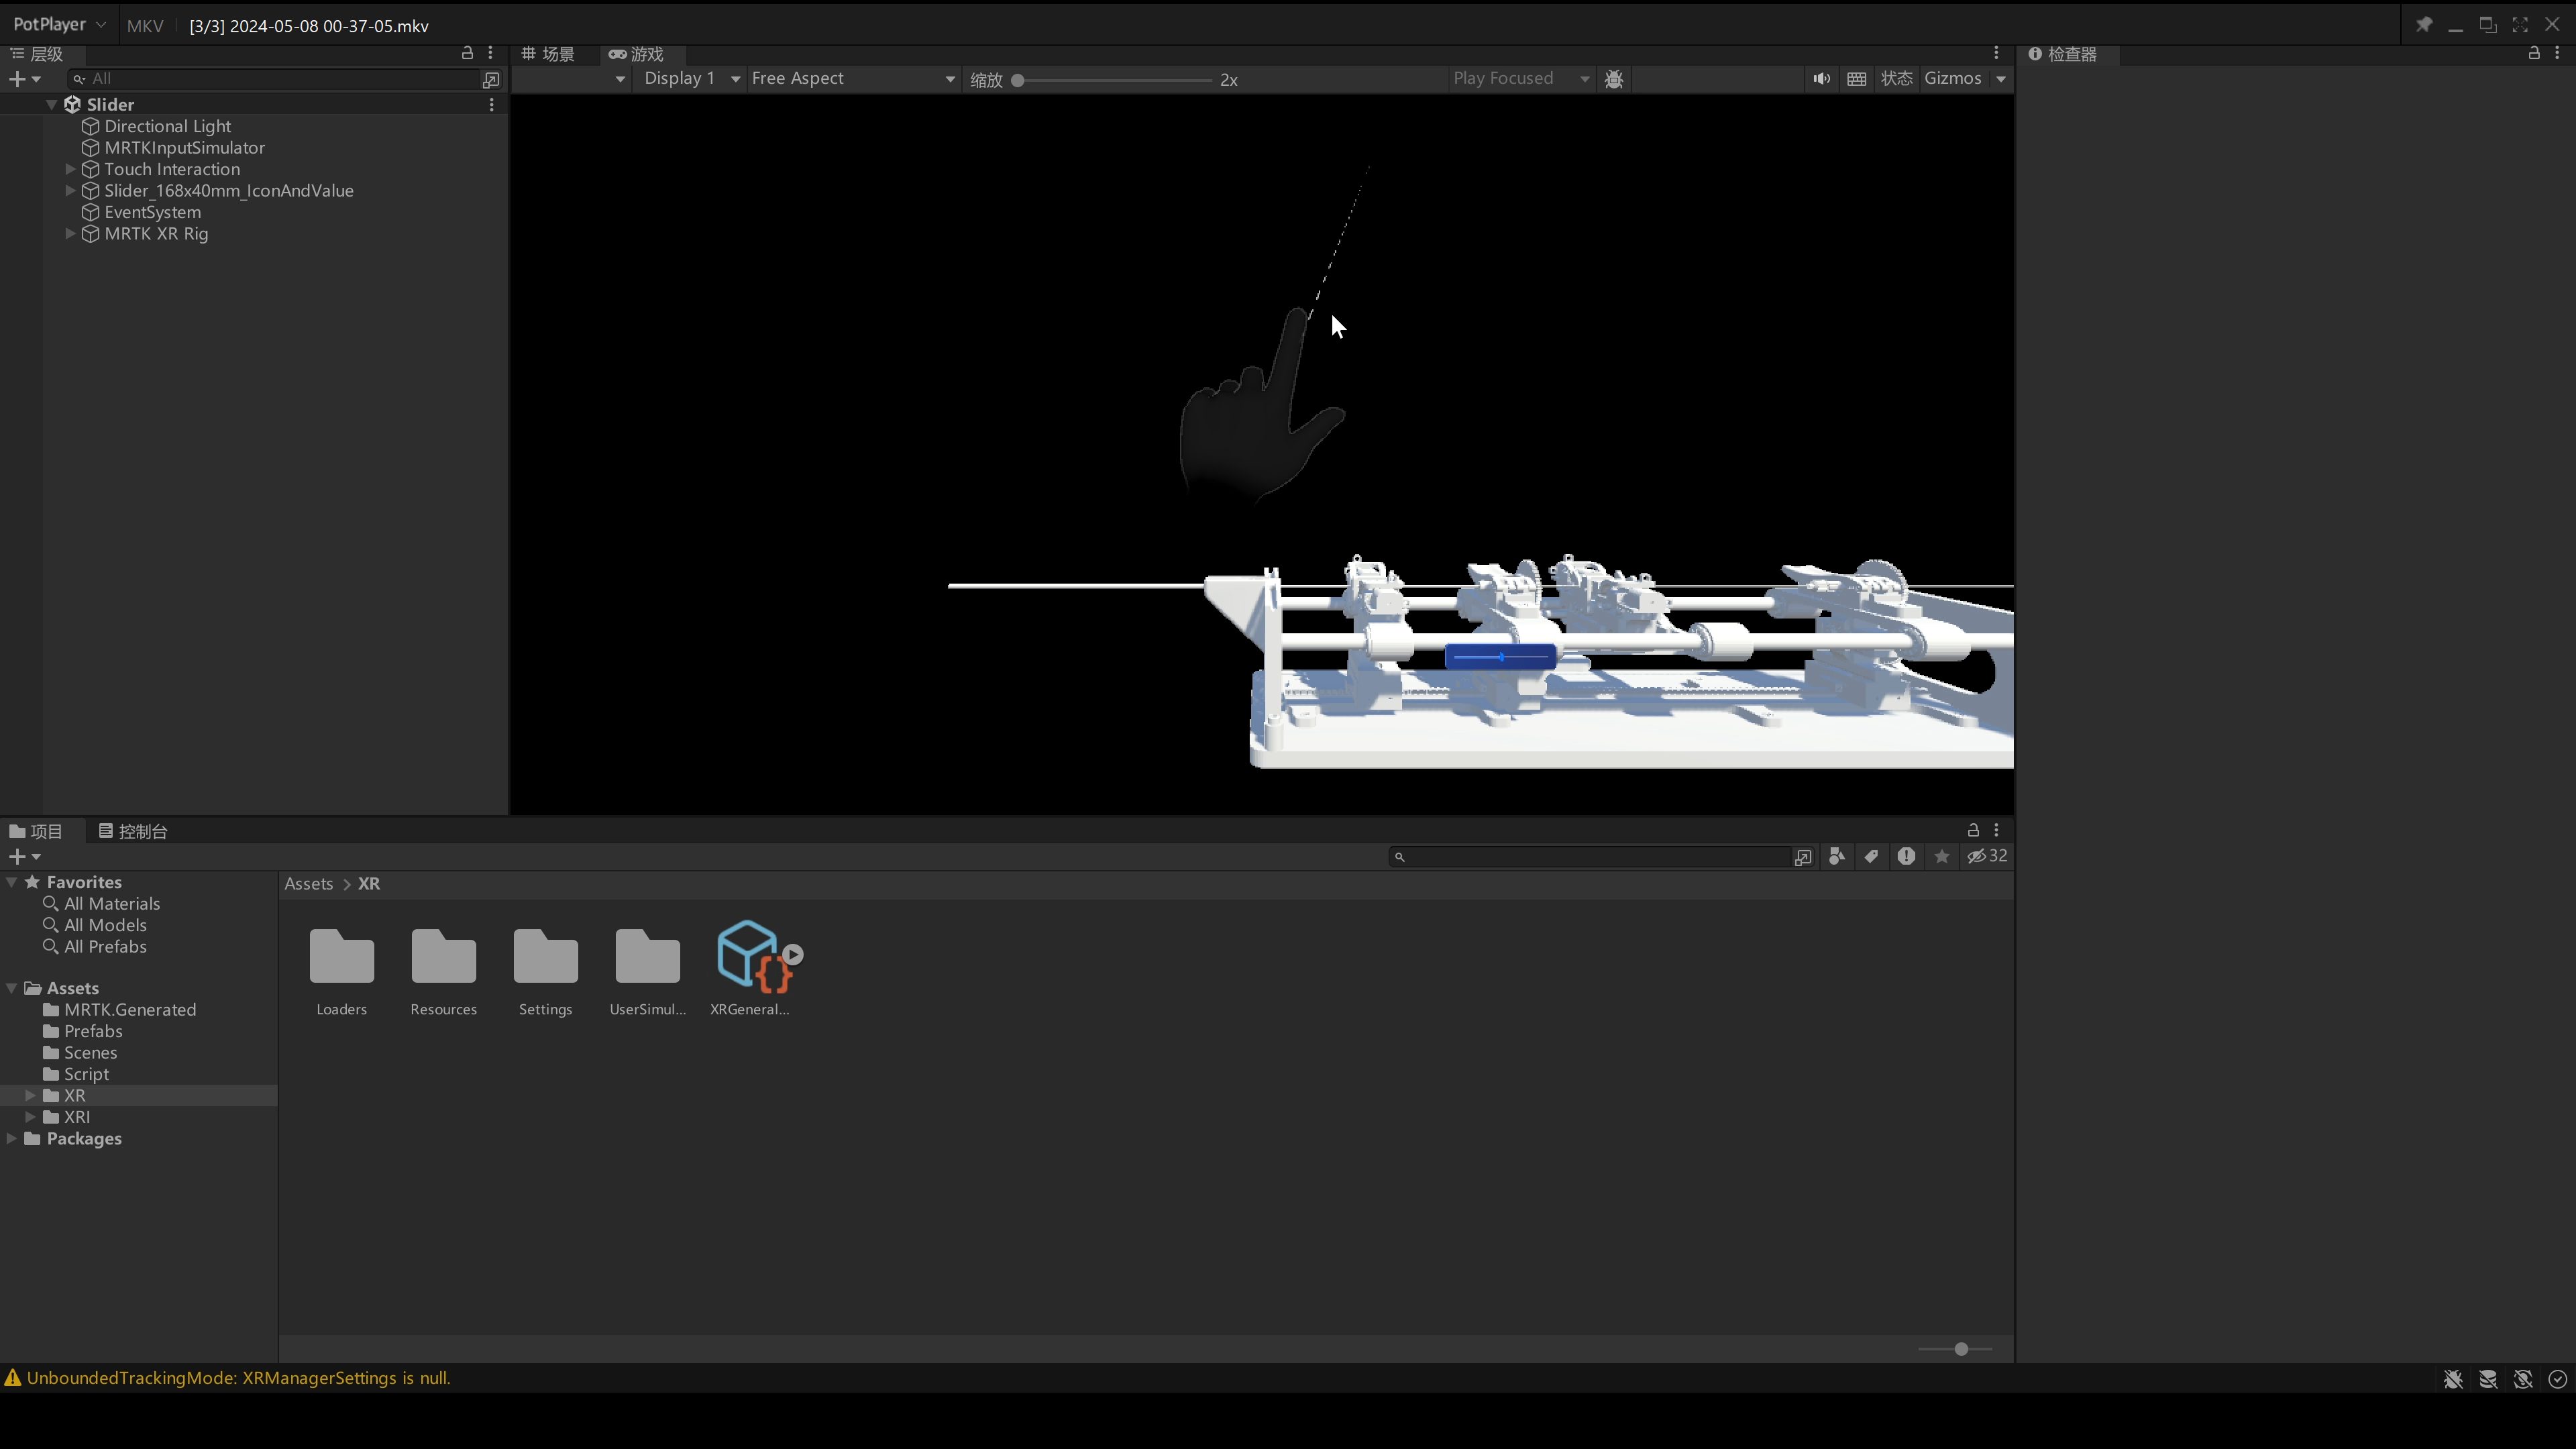
\includegraphics[width=0.8\textwidth]{hand1.png}
            \caption{Virtual Hand Control}
      \end{figure}
      \begin{figure}[H]
            \centering
            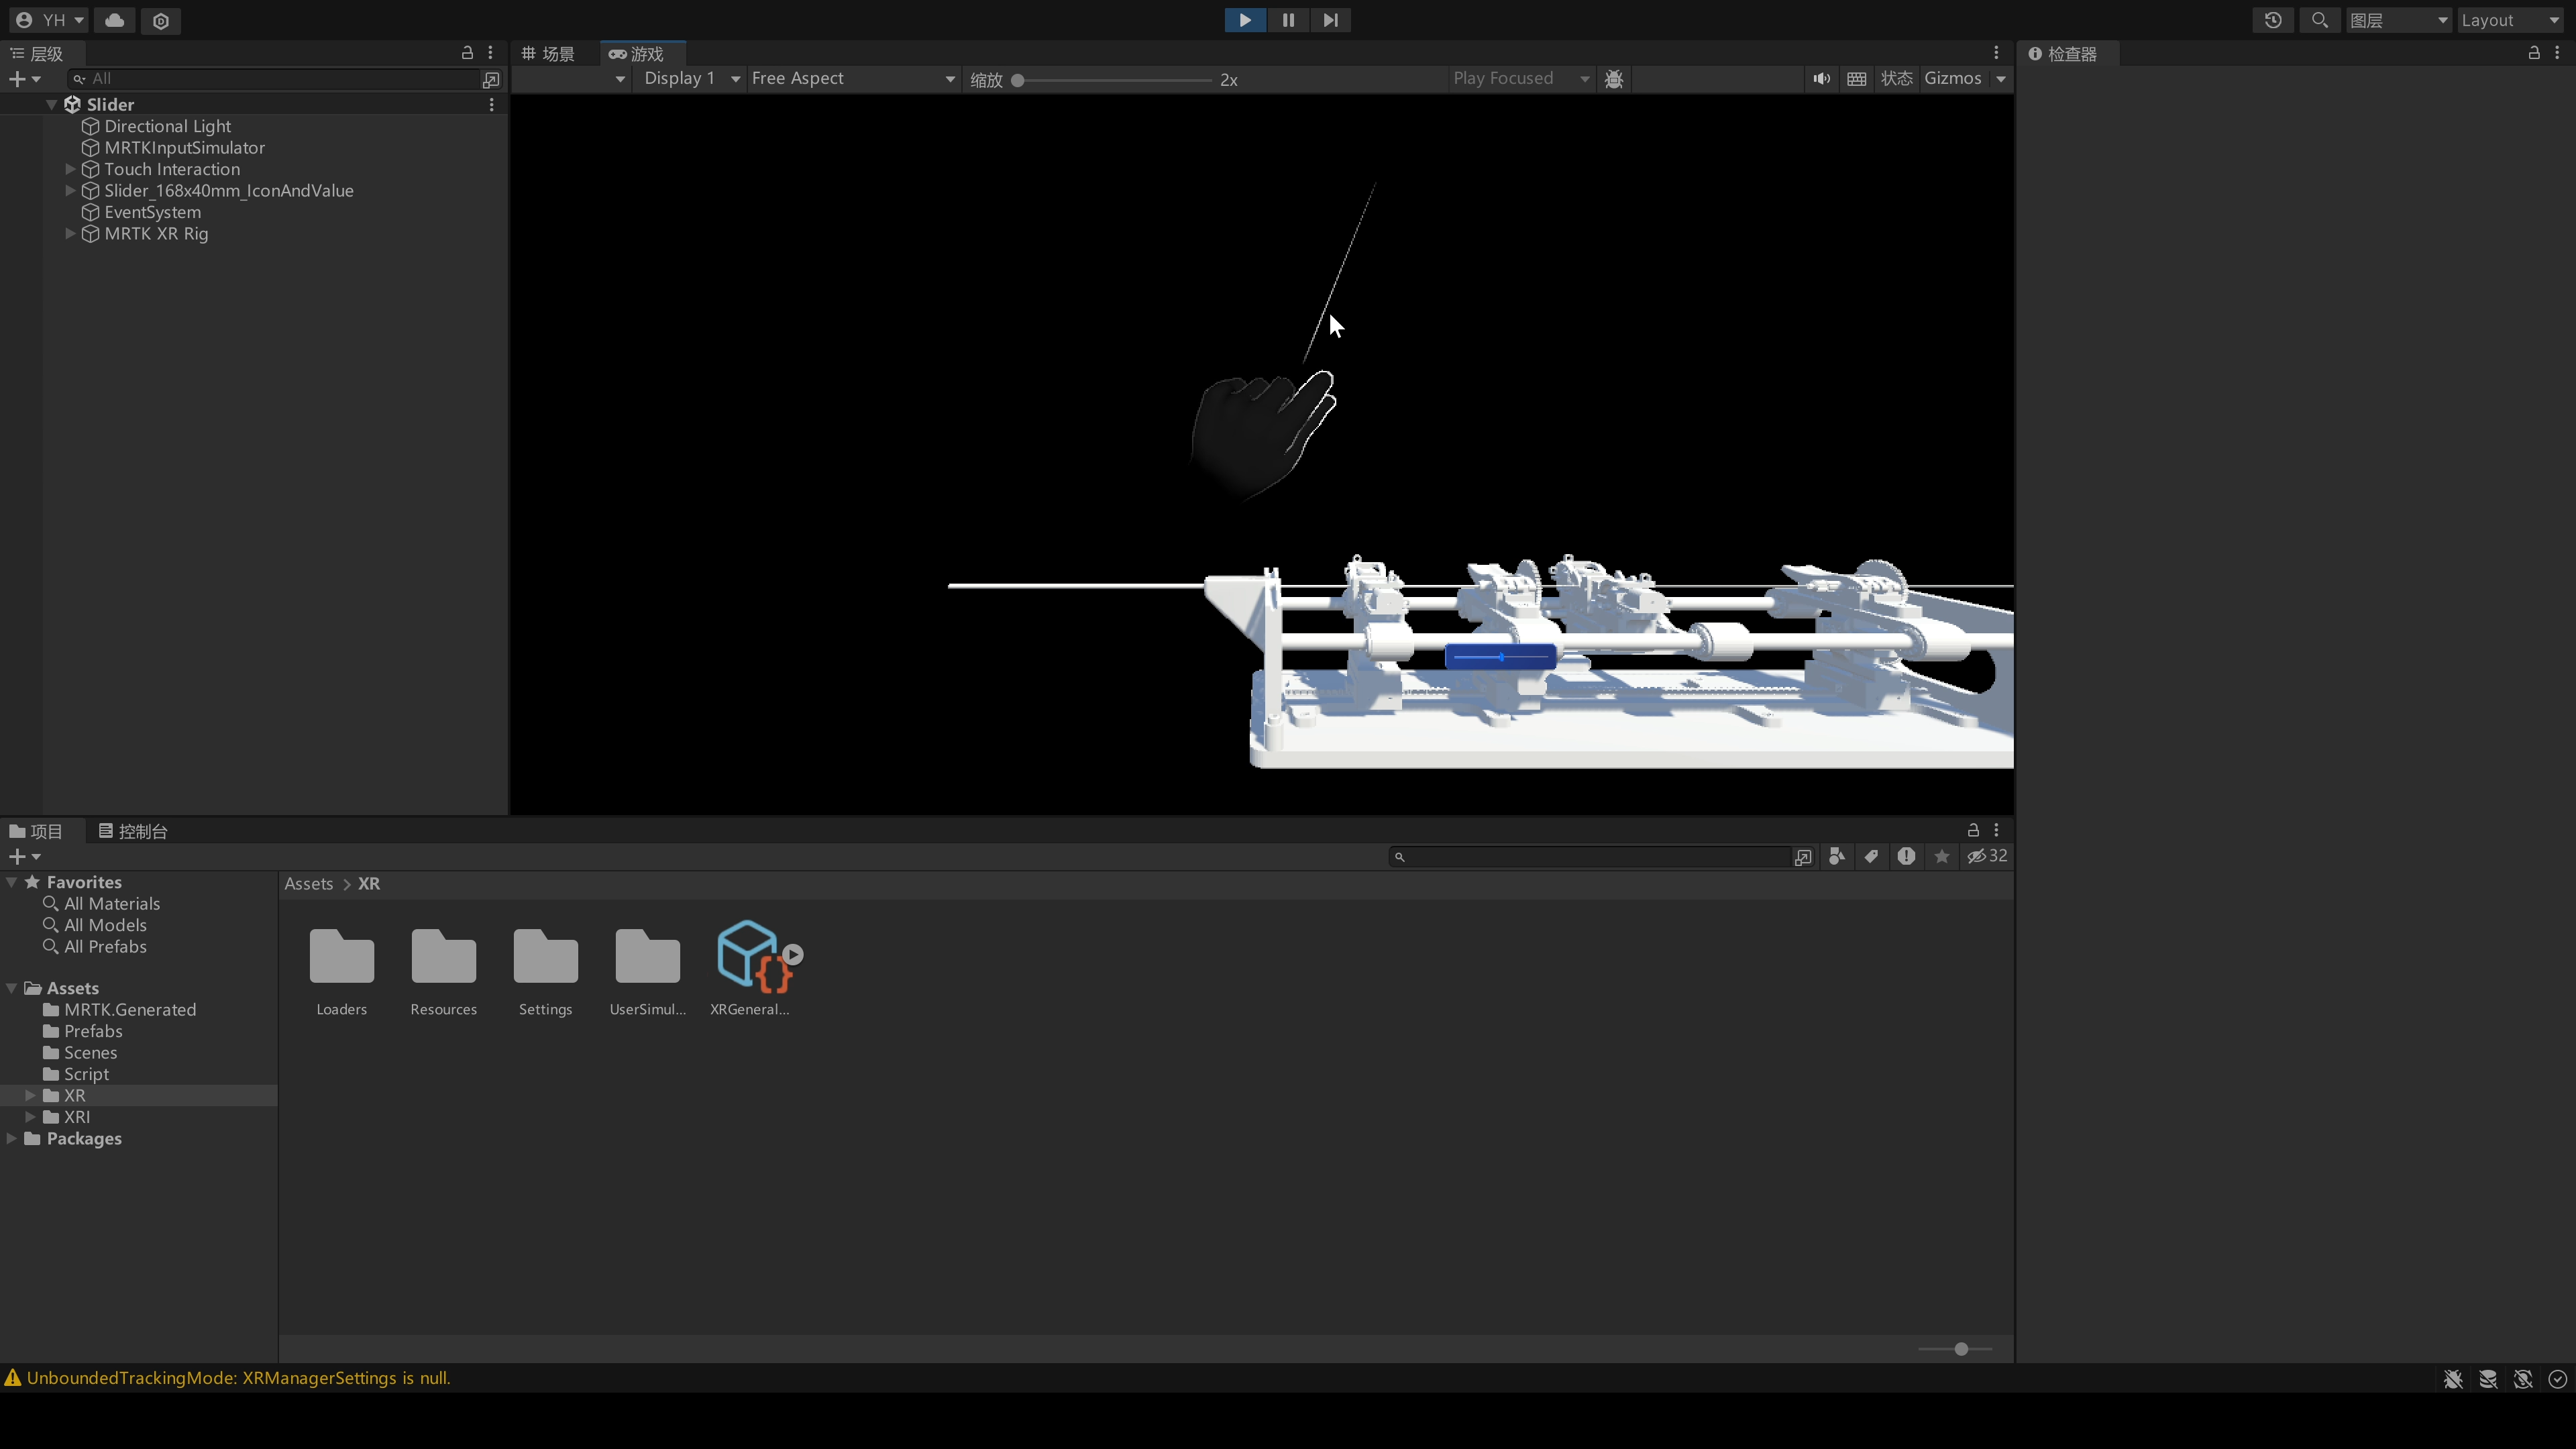
\includegraphics[width=0.8\textwidth]{hand2.png}
            \caption{Finger Pinching}
      \end{figure}
      \item \textbf{User Interface Design}
      \\
      In the initial design of the project, I designed two different user interfaces, one for users using a flat display and one for users using VR/AR. In the interface designed for users using flat displays, the interaction is mostly realised using buttons, whereas the interface designed for VR/AR users takes into account factors such as interaction in virtual environments and mostly uses a virtual interface for interaction.
      \begin{figure}[H]
            \centering
            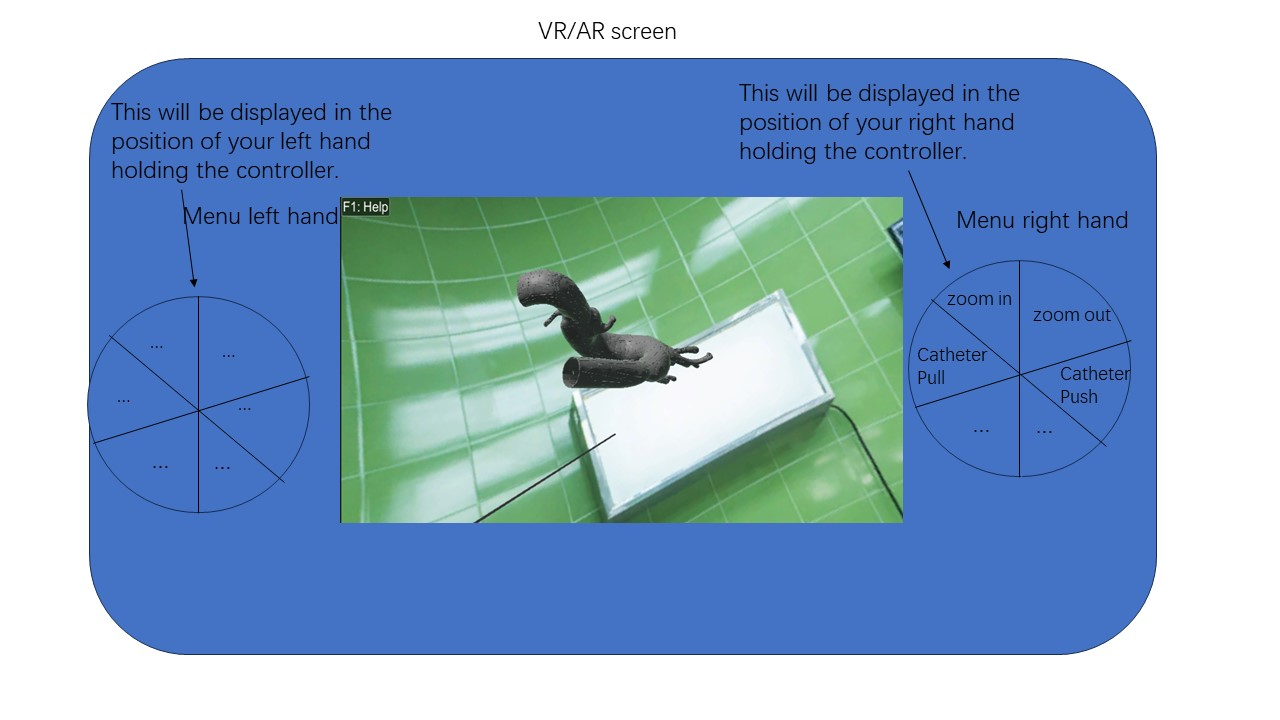
\includegraphics[width=0.8\textwidth]{UIUX.jpg}
            \caption{AR/VR User Interface}
      \end{figure}
      \begin{figure}[H]
            \centering
            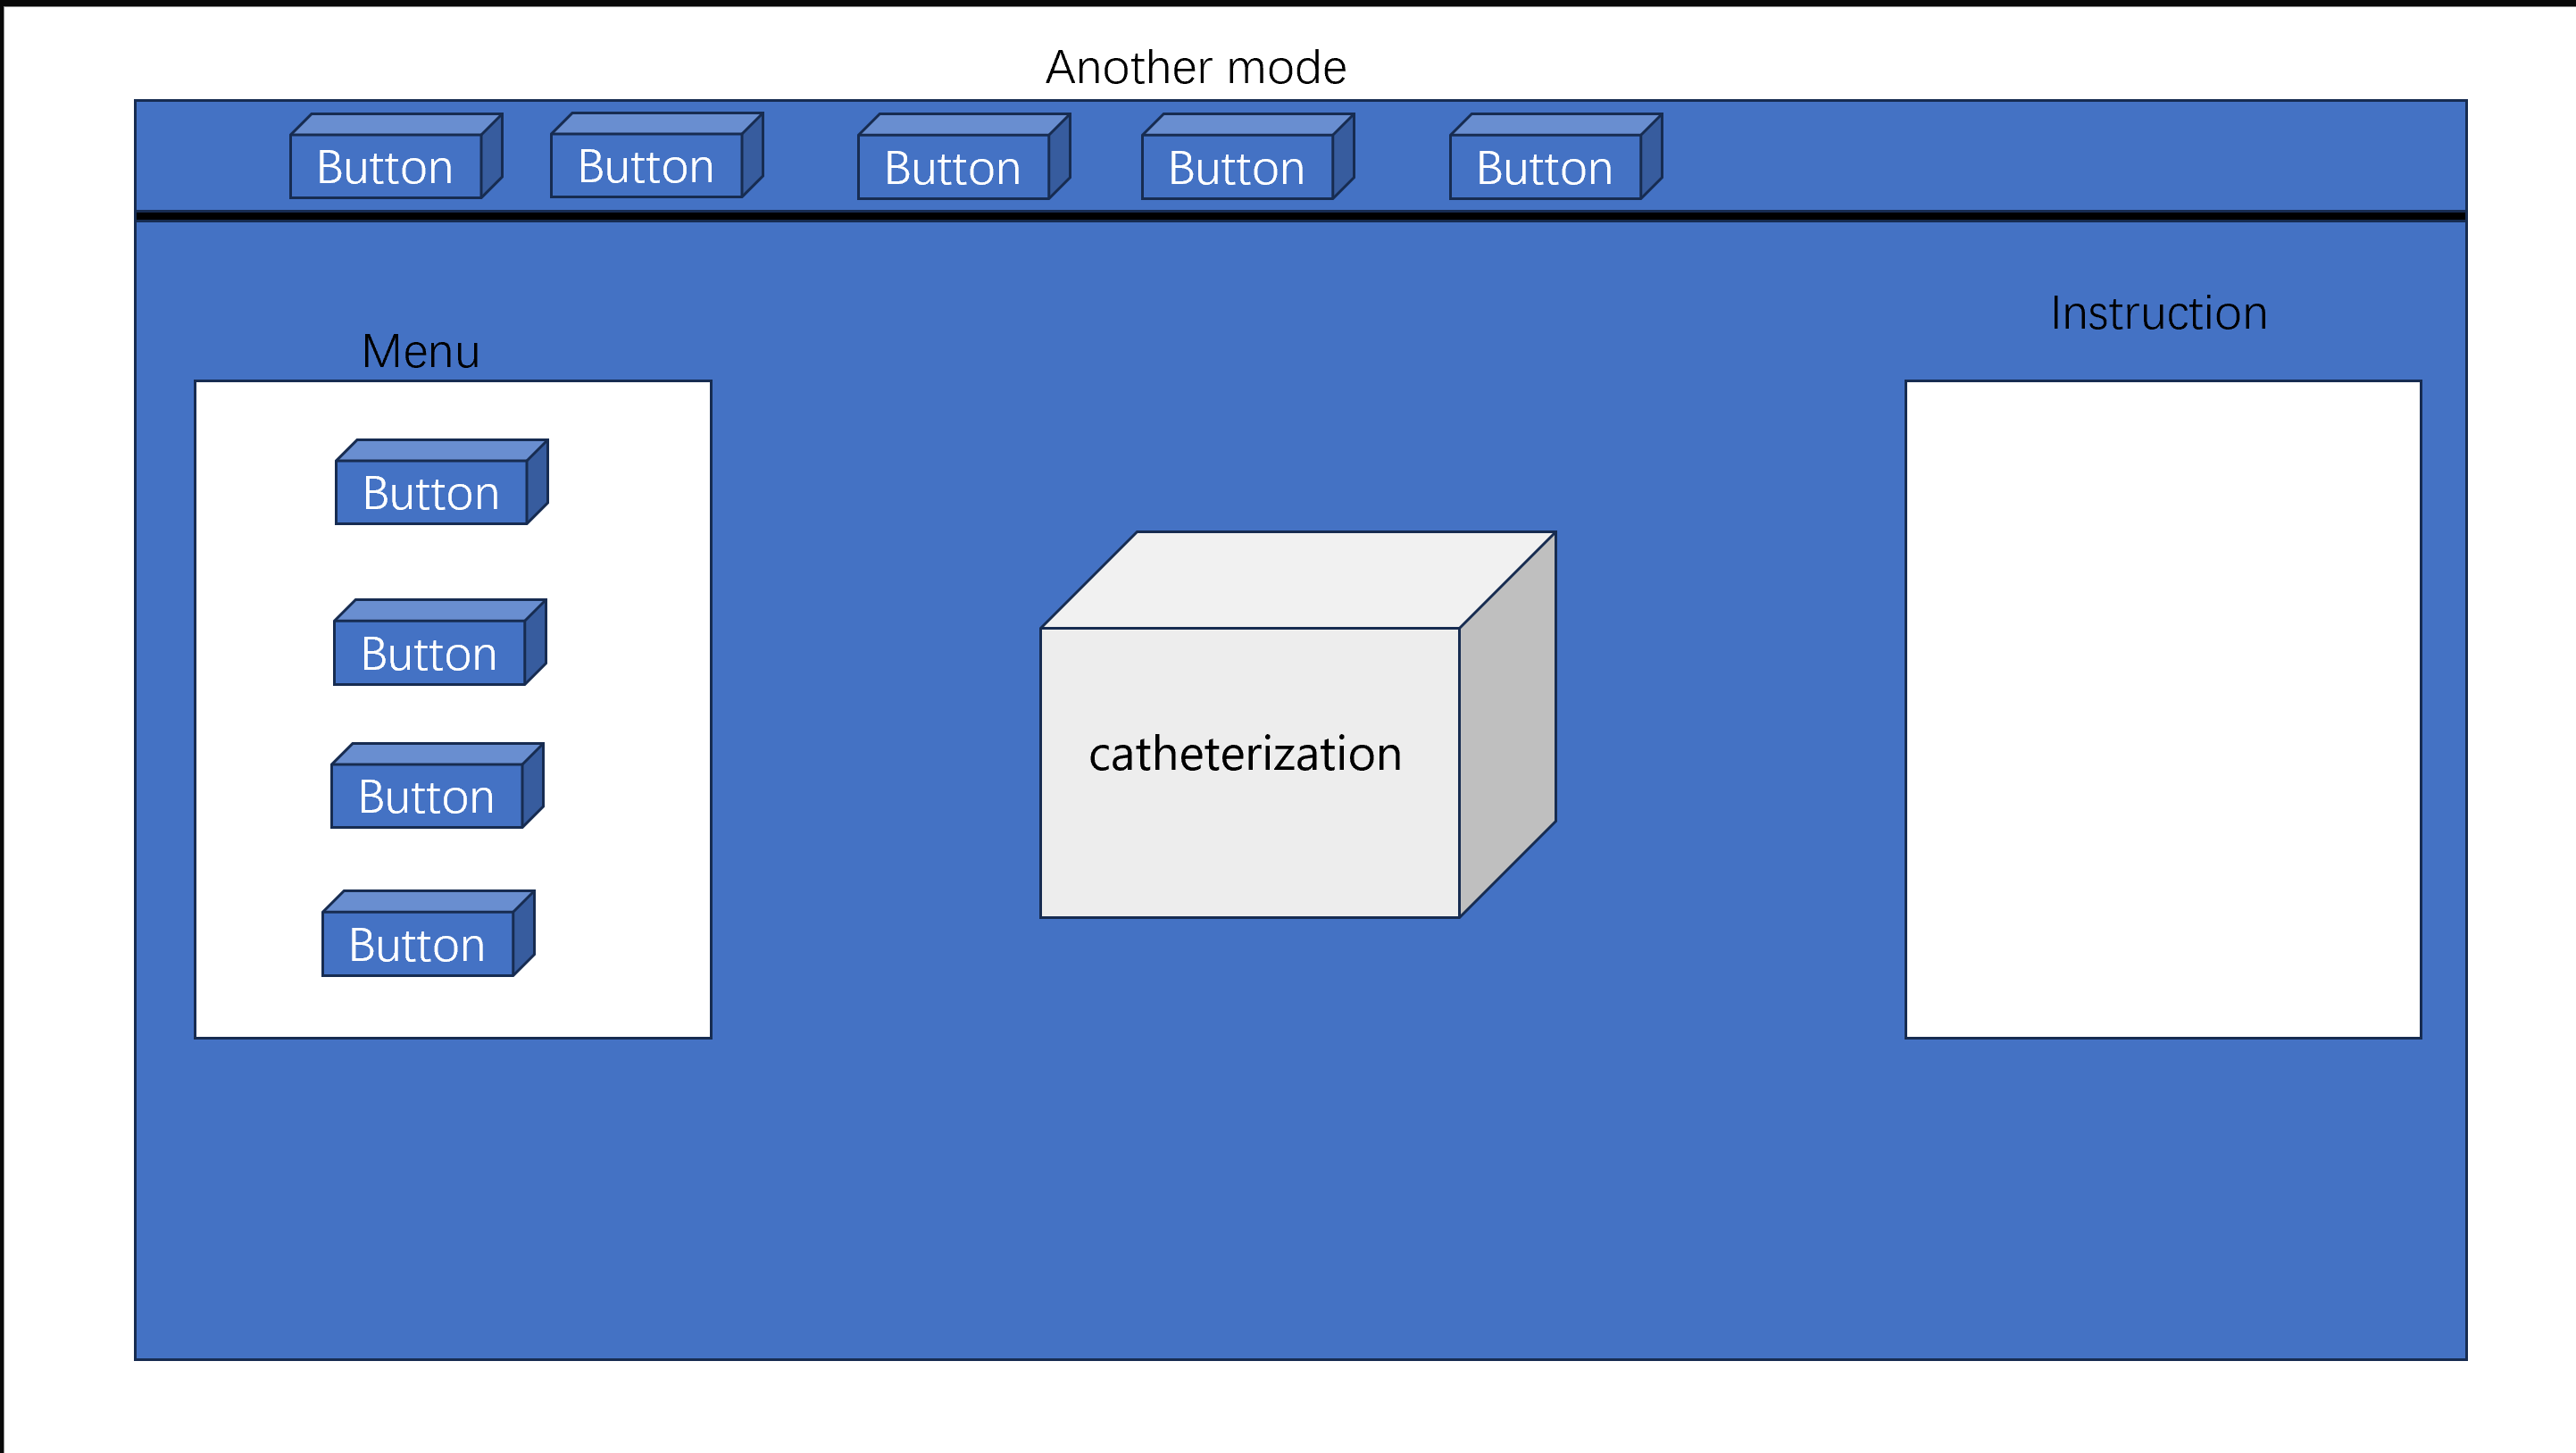
\includegraphics[width=0.8\textwidth]{uiux2.png}
            \caption{Flat Display User Interface}
      \end{figure}
      At this stage, the user interface is still in the design phase, as the core Endovascular Intervention Simulation component is still not up to the level of design that it was at the beginning of the project.
      
\end{enumerate}
\subsubsection{Implementation}
\label{sec:implementation}
\begin{enumerate}
      \item \textbf{Framework Implementation}
      \\
      The \gls{mrtk} development framework needs to be built in Unity first at the start of the project.
      \\\\
      First you need to download the \href{https://learn.microsoft.com/en-us/windows/mixed-reality/develop/unity/welcome-to-mr-feature-tool}{Mixed Reality Feature Tool for Unity} and select the corresponding Unity project and the necessary feature packs in the tool. The tool will then automatically add the required MRTK development packages to the project\cite{mrtk_m}.
      \begin{figure}[H]
            \centering
            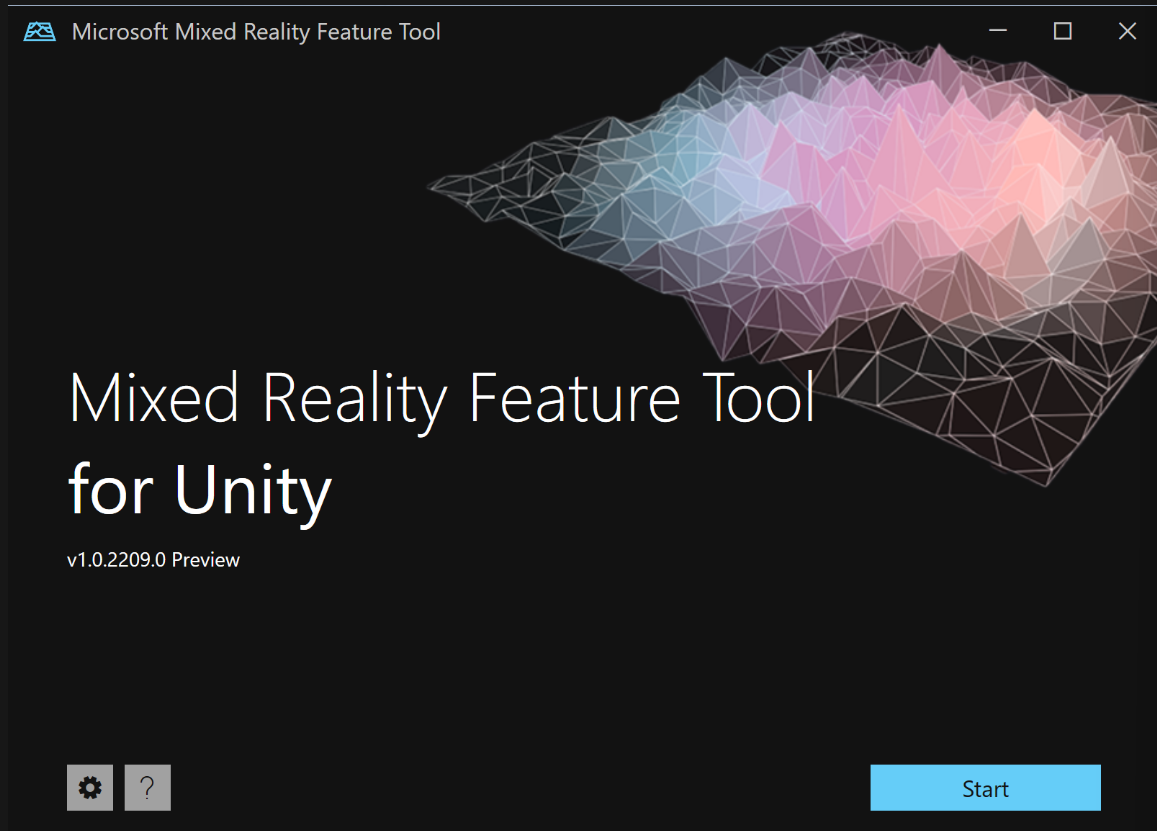
\includegraphics[width=0.8\textwidth]{mrtk1.png}
            \caption{Mixed Reality Feature Tool for Unity\cite{mrtk_m}}
      \end{figure}
      \begin{figure}[H]
            \centering
            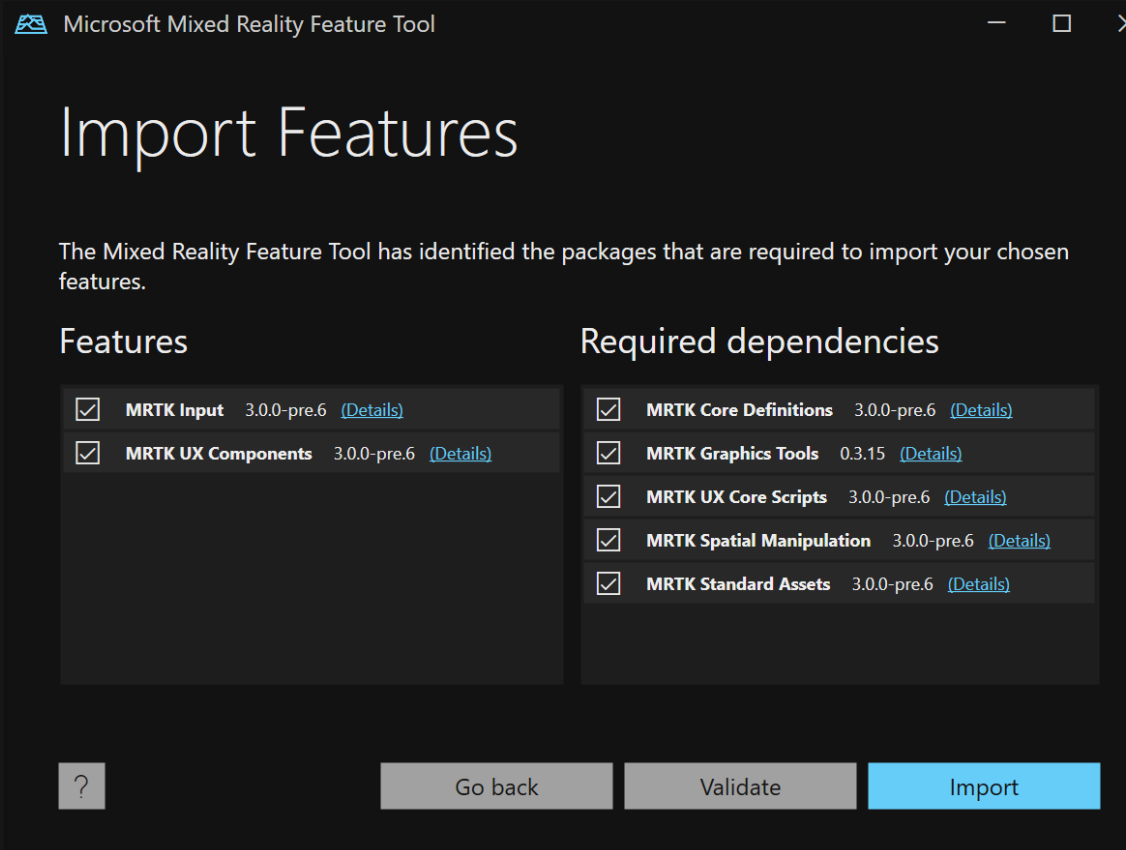
\includegraphics[width=0.8\textwidth]{mrtk2.png}
            \caption{Necessary Feature Packs\cite{mrtk_m}}
      \end{figure}
      In order to use this toolkit in the project, it needs to add the components \emph{MRTK XR Big} and \emph{MRTKInputSimulator} to the Asset for Unity. These components provide the necessary functionality to develop in HoloLens, such as hand simulation.
      \begin{figure}[H]
            \centering
            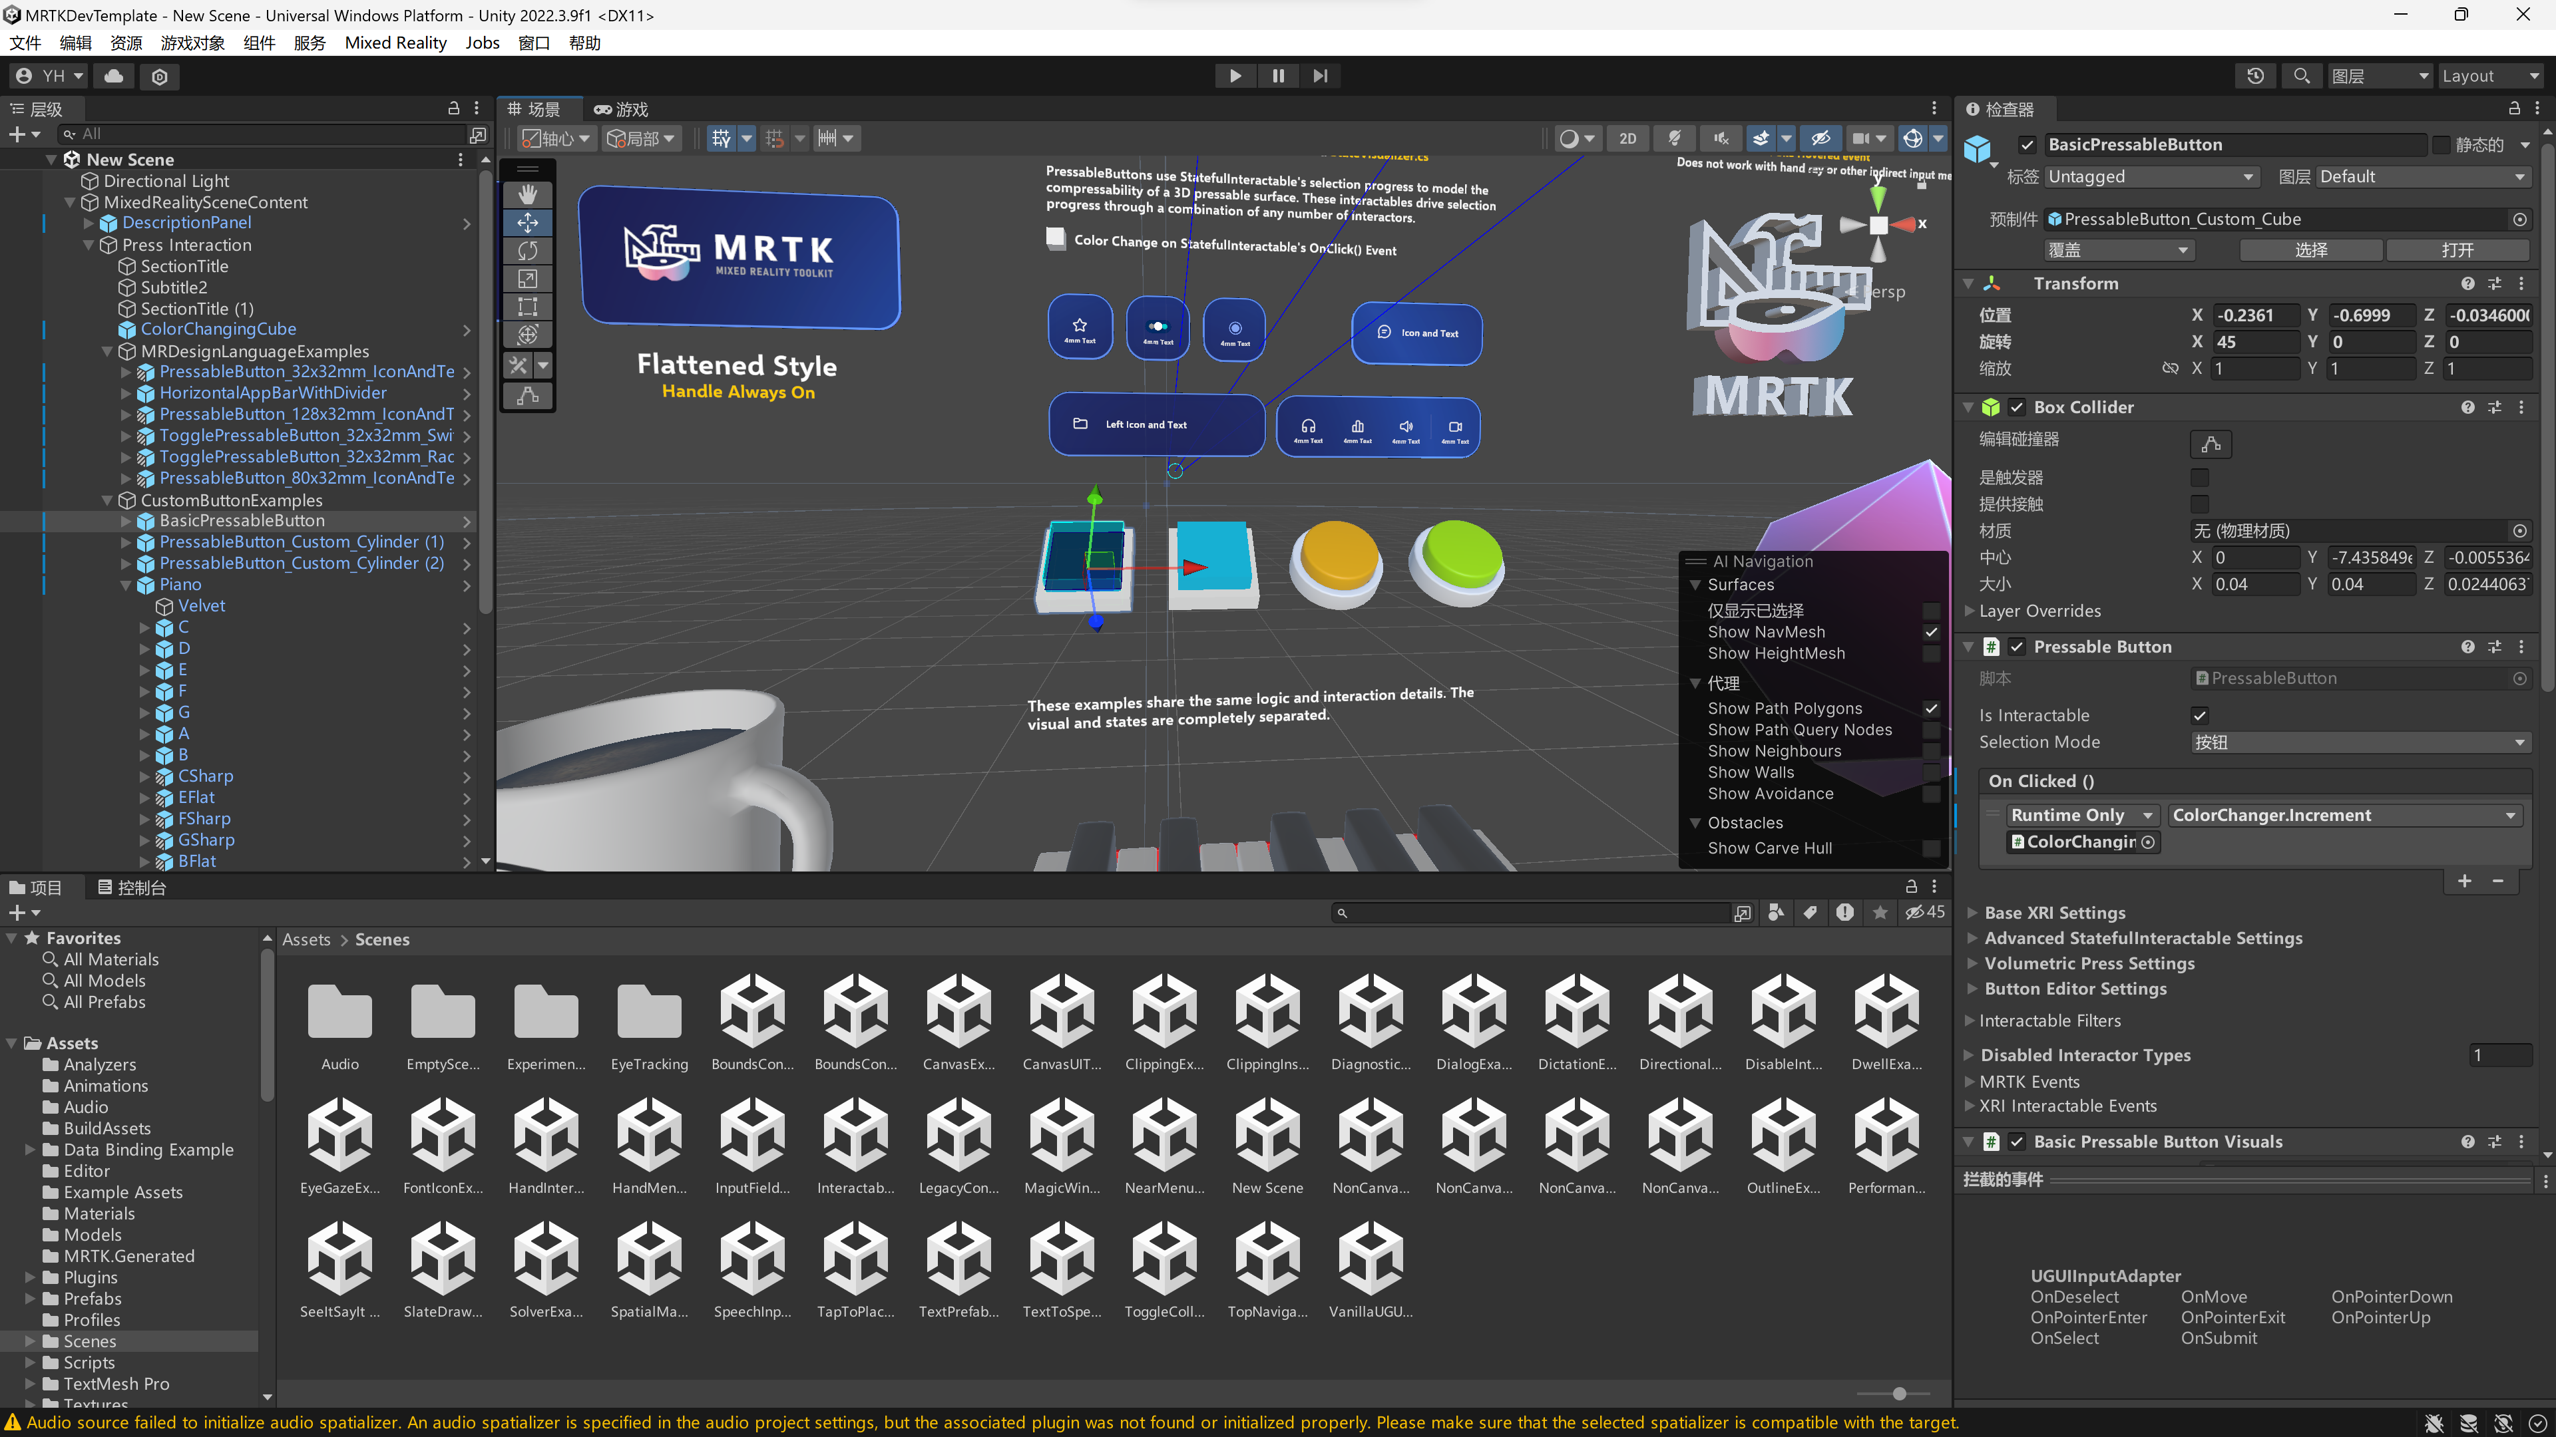
\includegraphics[width=0.8\textwidth]{mrtk_learn.png}
            \caption{MRTK3 Framework Example\cite{mrtk_m}}
      \end{figure}
      \item \textbf{Rope Implementation}
      \\
      As described in the Rope construction method described in the \hyperref[sec:rope]{Rope Design} section, the Rope construction was ultimately implemented using a method of splicing multiple Cubes using Unity C\# scripts.
      \\\\
      First create a Cube as a rope \emph{fragment prefab} and add the \emph{BoxCollider} component to give it a collision volume. It also needs to have the \emph{Rigidbody} component added to it to give it properties such as gravity and force impact so that it can react to gravity and external forces. After that, the Rope is generated and controlled directly by the C\# script where the \emph{RopeController} class resides. A dynamic rope is modelled by physical and visual components.
      \begin{figure}[H]
            \centering
            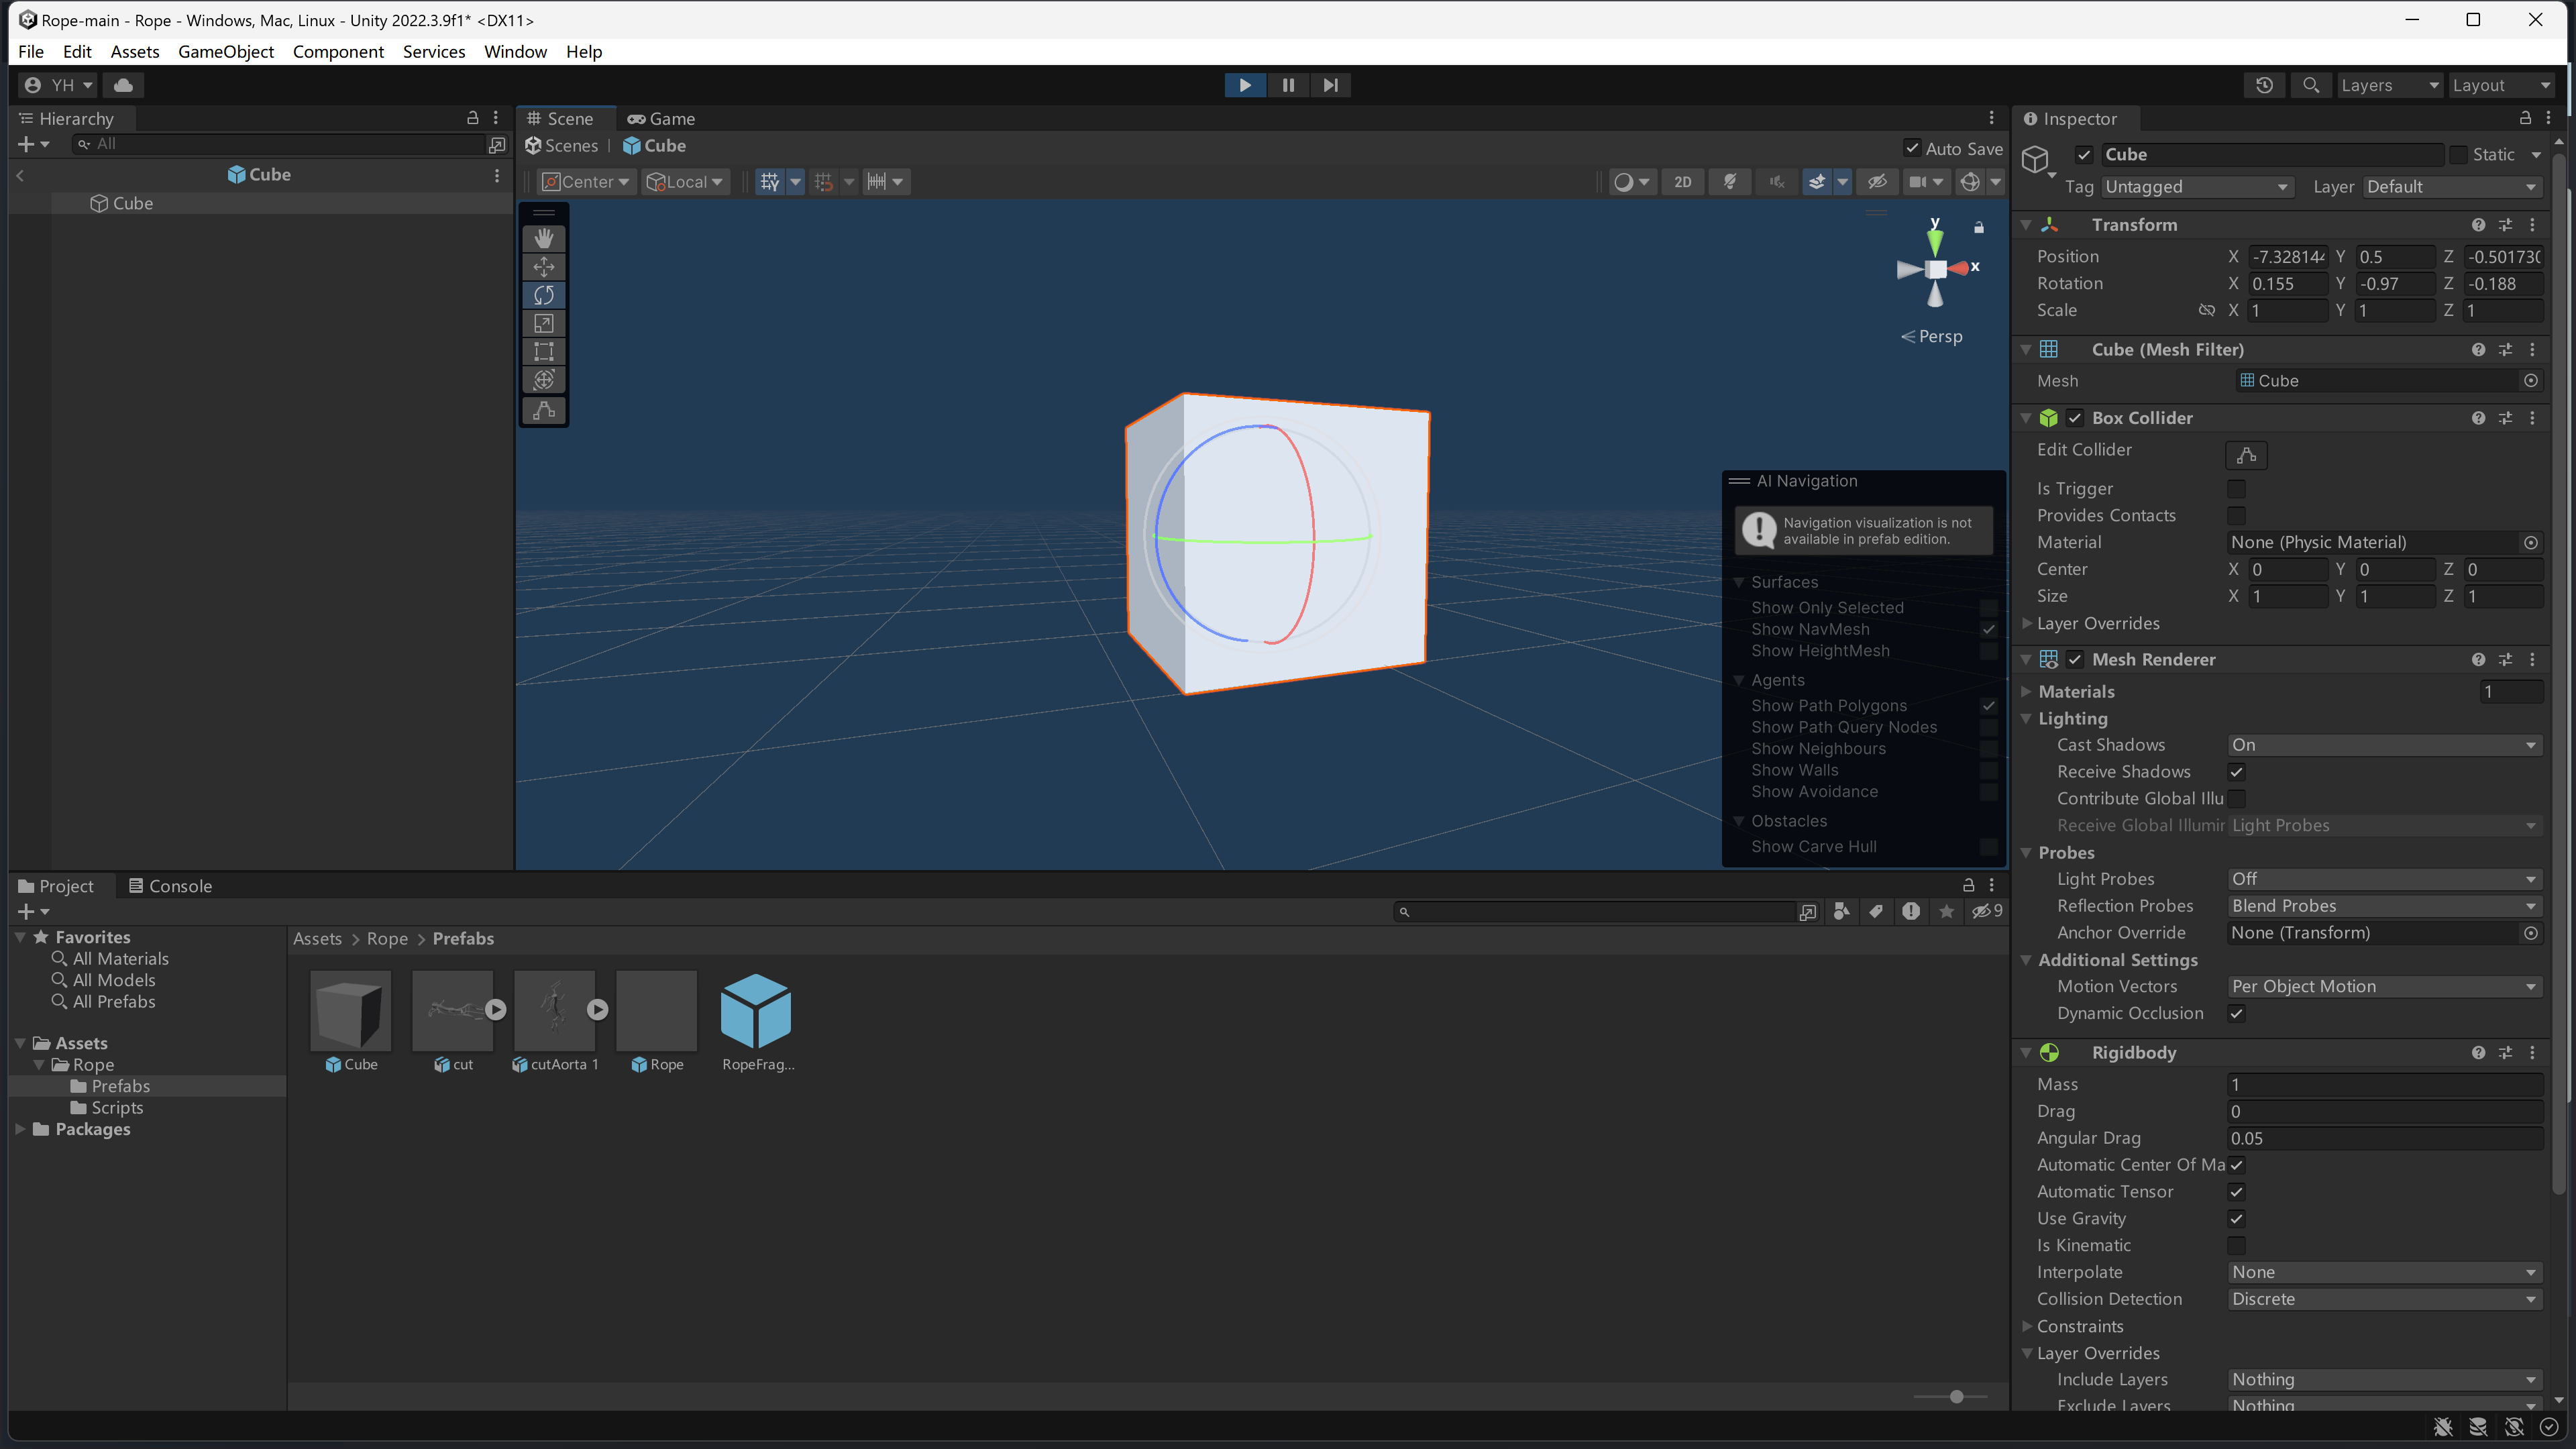
\includegraphics[width=0.8\textwidth]{cubezujian.png}
            \caption{Fragment Prefab}
      \end{figure}
      The class uses \emph{fragmentPrefab} to define each segment of the rope (using the previously created Cube), and \emph{fragmentCount } to control the total length of the rope, using the \emph{interval} variable to define the spatial distance between segments. They can all be modified in Unity editor configuration. In the script's Start method, it first initialises an array of \emph{GameObject} to store the rope segments (all cloned from the same Cube). Each segment is then instantiated and placed one by one in a loop to form a linear structure. For each fragment that is not the first, a \emph{FixedJoint } component is added to it. A \emph{FixedJoint} is a special type of physical joint that is used to fix two objects together in terms of their physical behaviour so that they behave as a single unit in the simulation environment\cite{UnityFixedJoint2024}. When a FixedJoint is used to connect two objects, the two objects remain relatively unchanged in position and orientation, simulating an effect of being pinned or welded together. This is later connected to the \emph{Rigidbody} component created by the previous fragment, achieving physical adhesion between the fragments.
      \begin{figure}[H]
            \centering
            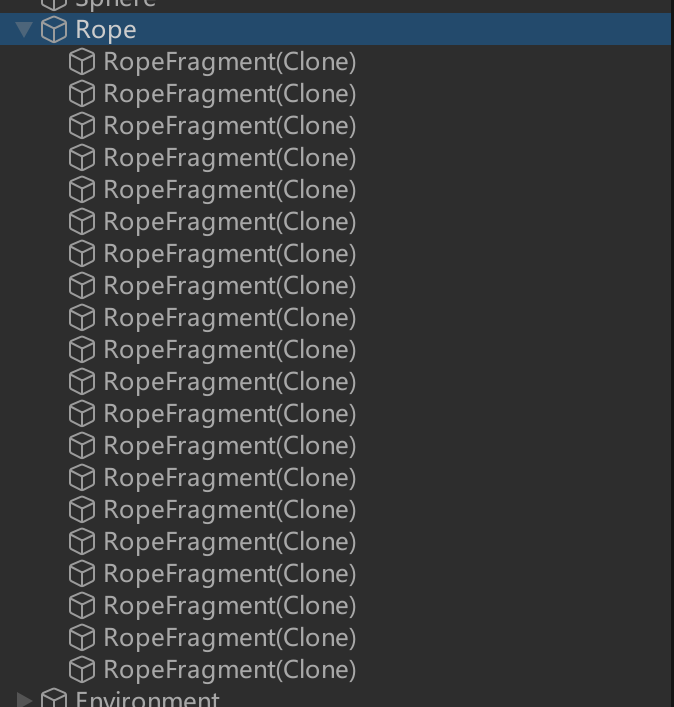
\includegraphics[width=0.5\textwidth]{rope colon.png}
            \caption{Fragment Prefab Connected }
      \end{figure}
      \begin{figure}[H]
            \centering
            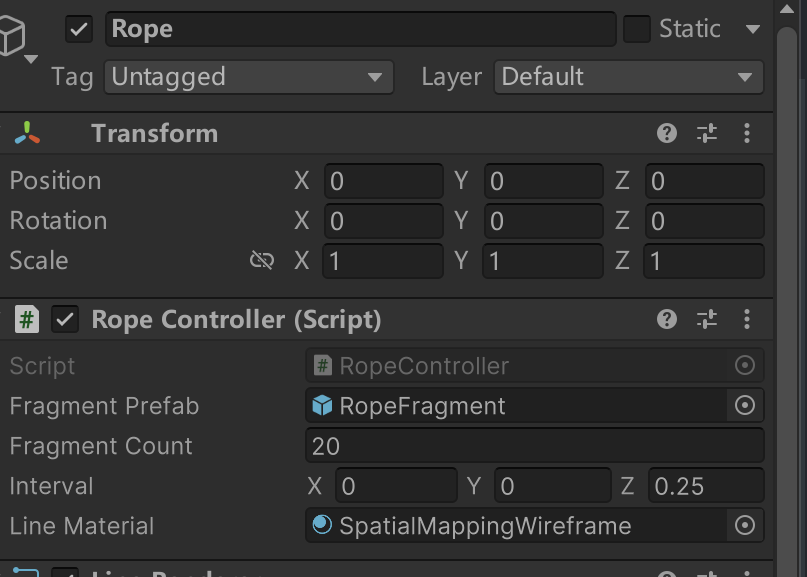
\includegraphics[width=0.5\textwidth]{rope setting.png}
            \caption{Rope Settings}
      \end{figure}
      Additionally, the same configuration that handles the initial bending of the rope is implemented in the script, whereby if a segment needs to have a bend applied, a trigonometric function is used to determine the offset of each segment by calculating the bending angle and the spacing of the segments of the rope. Specifically, it converts the total bending angle to radians for each segment, and then calculates to obtain offsets in the X and Z directions to visually realise the bending effect of the rope.
      \begin{figure}[H]
            \centering
            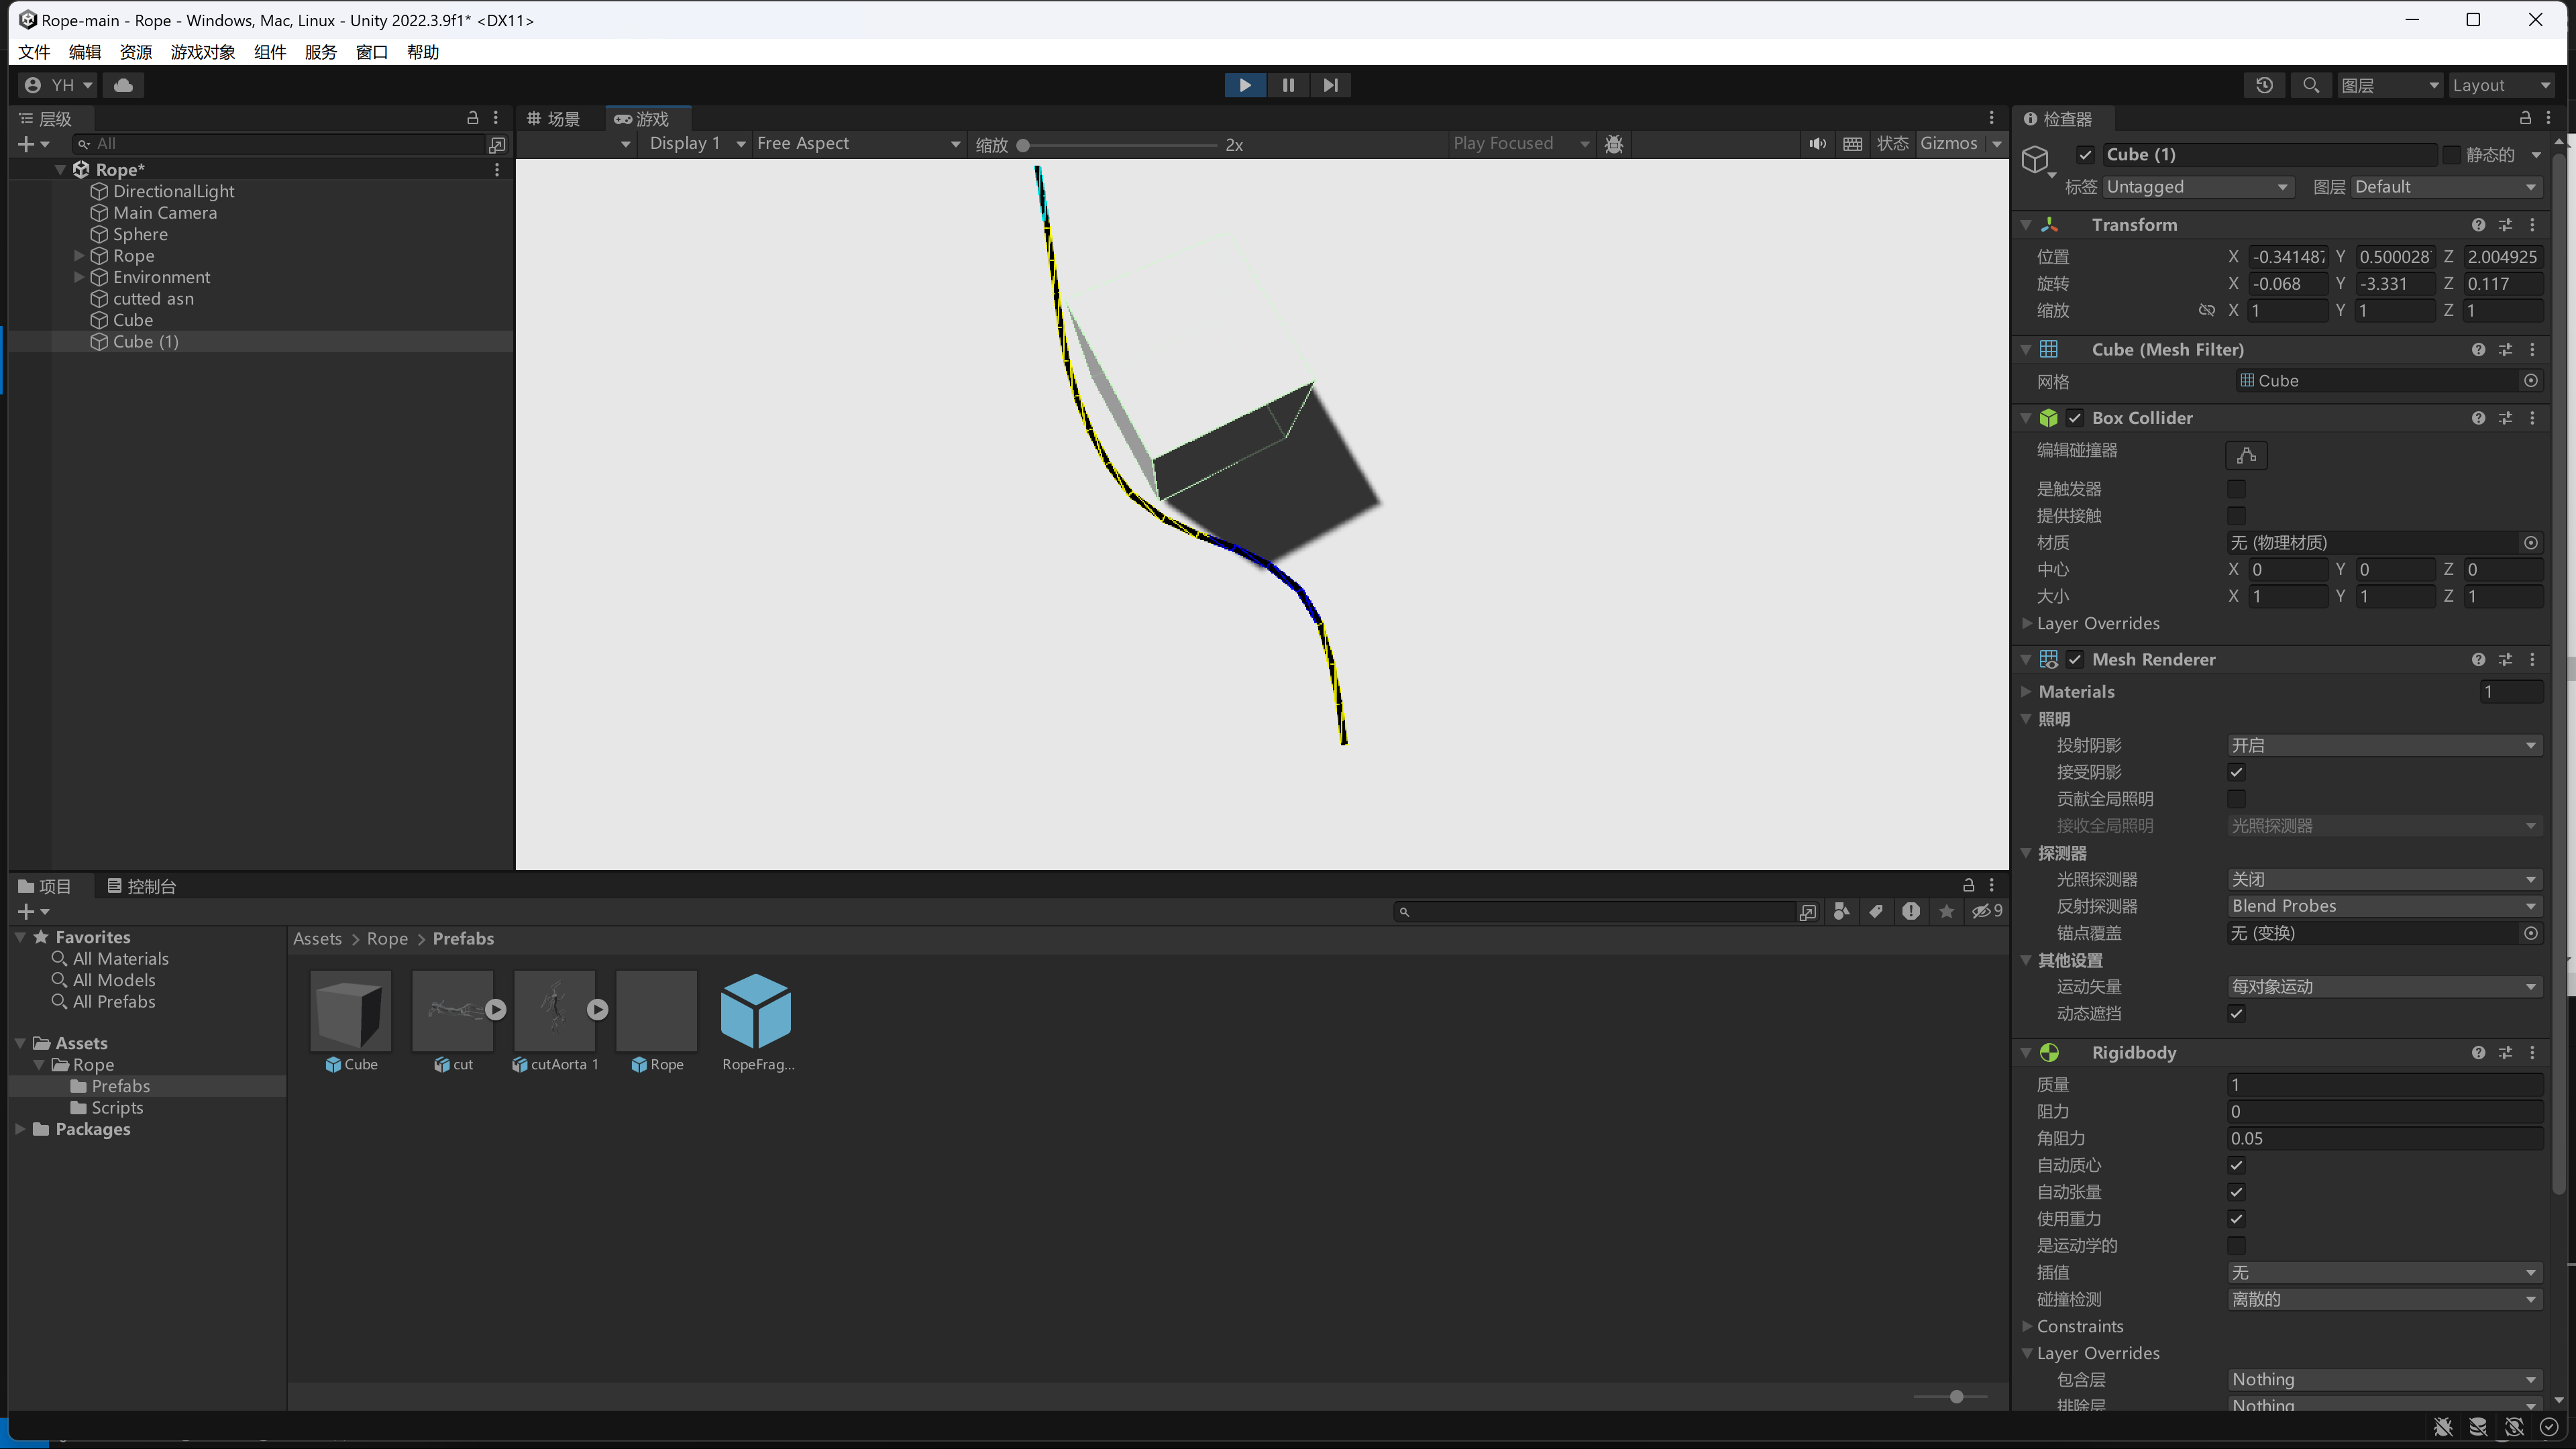
\includegraphics[width=0.8\textwidth]{React.png}
            \caption{Rope Bending}
      \end{figure}
      Also, in order to simulate the real Endovascular Intervention, the anterior end of the Rope is bent to a certain extent. By setting \emph{bendAngle} and \emph{segmentToBend}, some segments of the anterior end of the Rope can be bent to achieve a more realistic simulation.
      \\\\
      Finally, to enhance the visual representation of the rope, a \emph{LineRenderer} component is added to the script that draws a continuous line between the rope segments. This can also be adjusted in the Unity editor by configuring properties such as material, line width and colour to ensure that the rope is visually appealing. In the \emph{LateUpdate } method, the script dynamically updates the position of each point of the \emph{LineRenderer} based on the real-time physical position of the segments to ensure that the line is updated as the segments move, ensuring visual continuity and dynamic response.
      \begin{figure}[H]
            \centering
            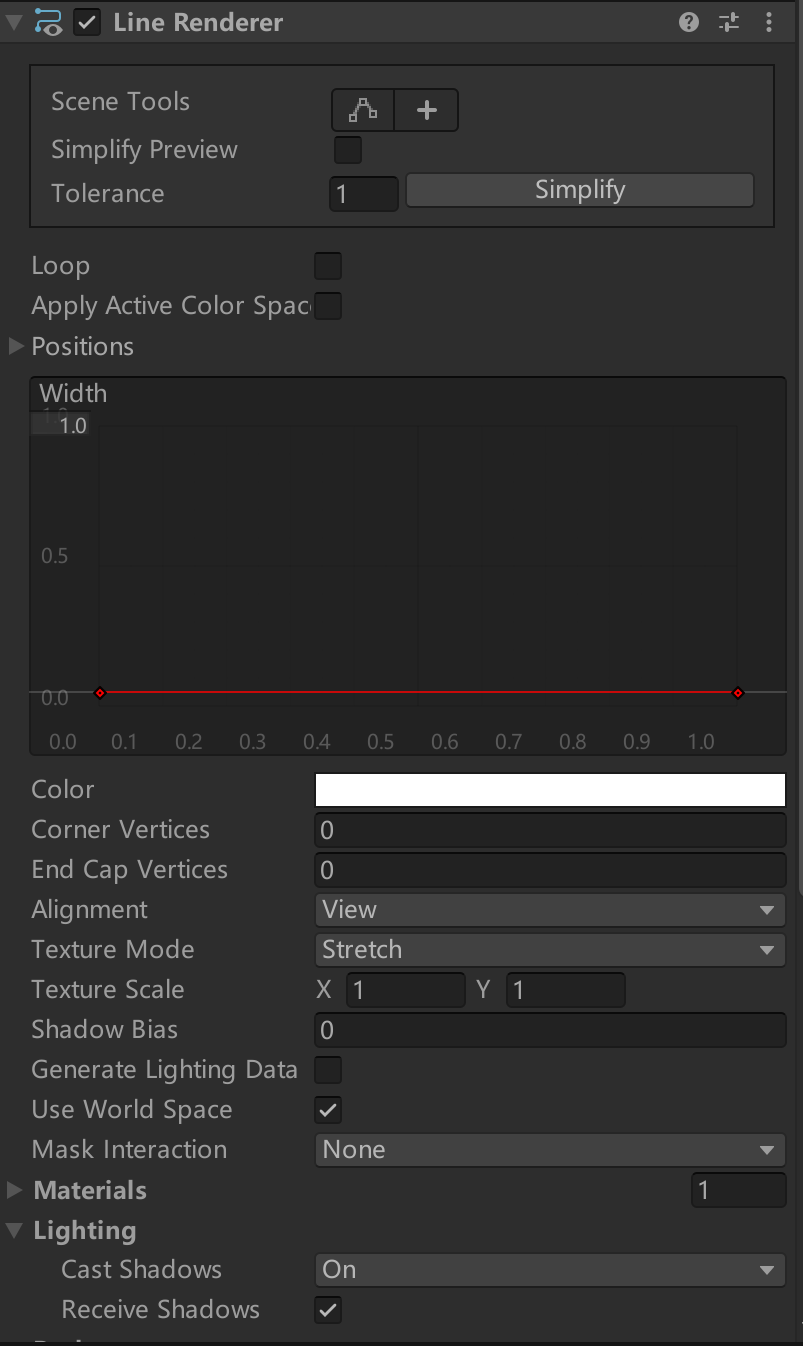
\includegraphics[width=0.5\textwidth]{render.png}
            \caption{Line Renderer}
      \end{figure}
      \paragraph{Pseudocode for the Rope Implementation:}
      \begin{minted}[frame=single, linenos=true, fontsize=\footnotesize]{C}
using UnityEngine;

namespace Rope
{
    public class RopeController : MonoBehaviour
    {
        [SerializeField] private GameObject fragmentPrefab;
        [SerializeField] private int fragmentCount = 80;
        [SerializeField] private Vector3 interval = new Vector3(0f, 0f, 0.25f);
        [SerializeField] private Material lineMaterial; 

        private GameObject[] fragments;
        private float[] xPositions;
        private float[] yPositions;
        private float[] zPositions;
        private CatmullRomSpline splineX;
        private CatmullRomSpline splineY;
        private CatmullRomSpline splineZ;
        private int splineFactor = 4;

        void Start()
        {
            fragments = new GameObject[fragmentCount];
            var position = Vector3.zero;
            // The desired total bend angle
            var bendAngle = 30f; 
            // Number of segments over which to apply the bend
            var segmentToBend = 0; 

            for (var i = 0; i < fragmentCount; i++)
            {
                fragments[i] = Instantiate(fragmentPrefab, 
                position, Quaternion.identity, transform);

                if (i > 0)
                {
                    var joint = 
                    fragments[i].AddComponent<FixedJoint>();
                    joint.connectedBody = 
                    fragments[i - 1].GetComponent<Rigidbody>();
                }

                // Calculate the bend for the initial segments
                if (i < segmentToBend)
                {
                    // Convert the total angle into radians 
                    // and distribute it across the specified segments
                    var radiansPerSegment = 
                    Mathf.Deg2Rad * (bendAngle / segmentToBend);
                    // Use interval.z as the base distance between segments
                    var offsetX = Mathf.Sin(radiansPerSegment * i) * 
                    interval.z; 
                    var offsetZ = 
                    (1 - Mathf.Cos(radiansPerSegment * i)) * interval.z;

                    // Apply the calculated offset
                    position.x += offsetX;
                    position.z += offsetZ;
                }
                else
                {
                    position += interval;
                }
            }

            var lineRenderer = GetComponent<LineRenderer>();\
            // Make sure a material is assigned
            lineRenderer.material = lineMaterial; 
            lineRenderer.startWidth = 0.05f;
            lineRenderer.endWidth = 0.05f;
            lineRenderer.positionCount = fragmentCount;
            lineRenderer.startColor = Color.white;
            lineRenderer.endColor = Color.white;
        }

        void LateUpdate()
        {
            var lineRenderer = GetComponent<LineRenderer>();

            for (int i = 0; i < fragmentCount; i++)
            {
                lineRenderer.SetPosition(i, fragments[i].transform.position);
            }
        }
    }
}
      \end{minted}
      \item \textbf{Model Implementation}
      \\
      To give the model a collision volume, you need to add \emph{Collider} to it. There are two types of \emph{Collider} in Unity, \emph{Box Collider} and \emph{Mesh Collider}.
      \\
      Box Collider is a simple collider component that is usually applied to objects with regular geometry, such as cubes, rectangles, and so on. This collider has a low computational cost due to its simple geometry and is suitable for scenarios that deal with a large number of object collisions. Its main advantages are high computational efficiency and low computational cost. \cite{UnityBoxCollider2024}
      \begin{figure}[H]
            \centering
            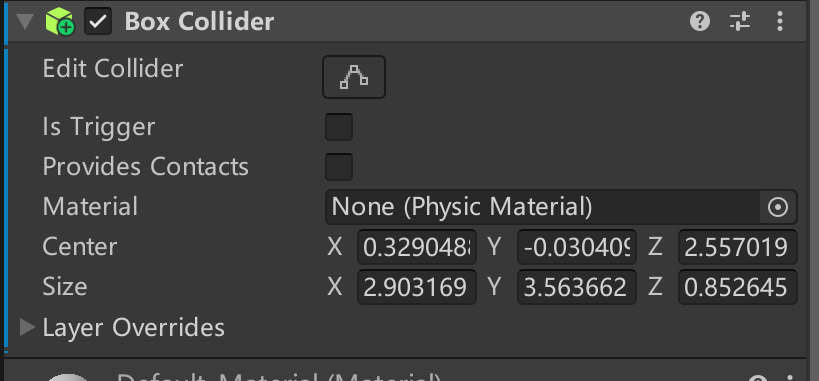
\includegraphics[width=0.5\textwidth]{box.png}
            \caption{Box Collider}
      \end{figure}
     
      Mesh Collider, on the other hand, is a collider component that can handle complex model shapes, and is suitable for objects with irregular shapes and a high level of detail, such as Aorta. since it creates collision zones based on the real mesh of the model, it can provide very accurate collision detection, but this also means a higher computational cost. \cite{UnityMeshCollider2024}
      \begin{figure}[H]
            \centering
            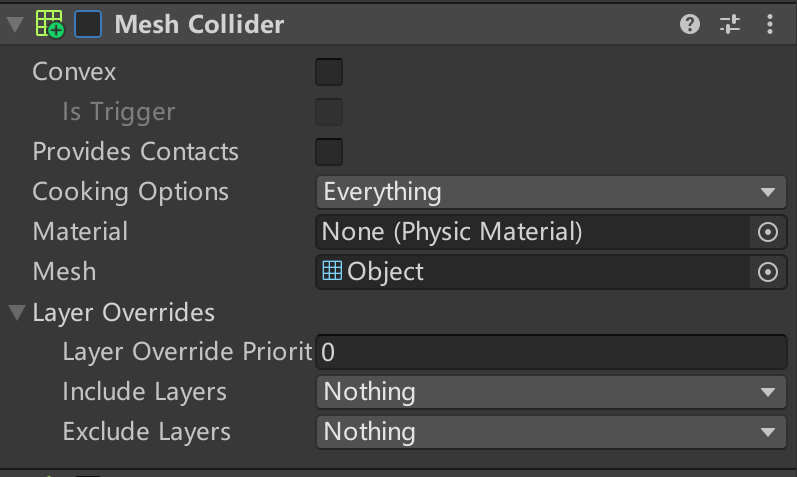
\includegraphics[width=0.5\textwidth]{mesh.png}
            \caption{Mesh Collider}
      \end{figure}
      In order to achieve more accurate interactions between Rope and Aorta, \emph{Mesh Collider} is used to achieve more detailed interactions, applying \emph{Mesh Collider} to the Aorta model and applying Aorta's mesh can achieve more accurate interactions. The image below shows the difference between using \emph{Box Collider} and \emph{Mesh Collider}, and it is clear that using \emph{Box Collider} does not allow Rope to enter the Aorta model.
      \begin{figure}[H]
            \centering
            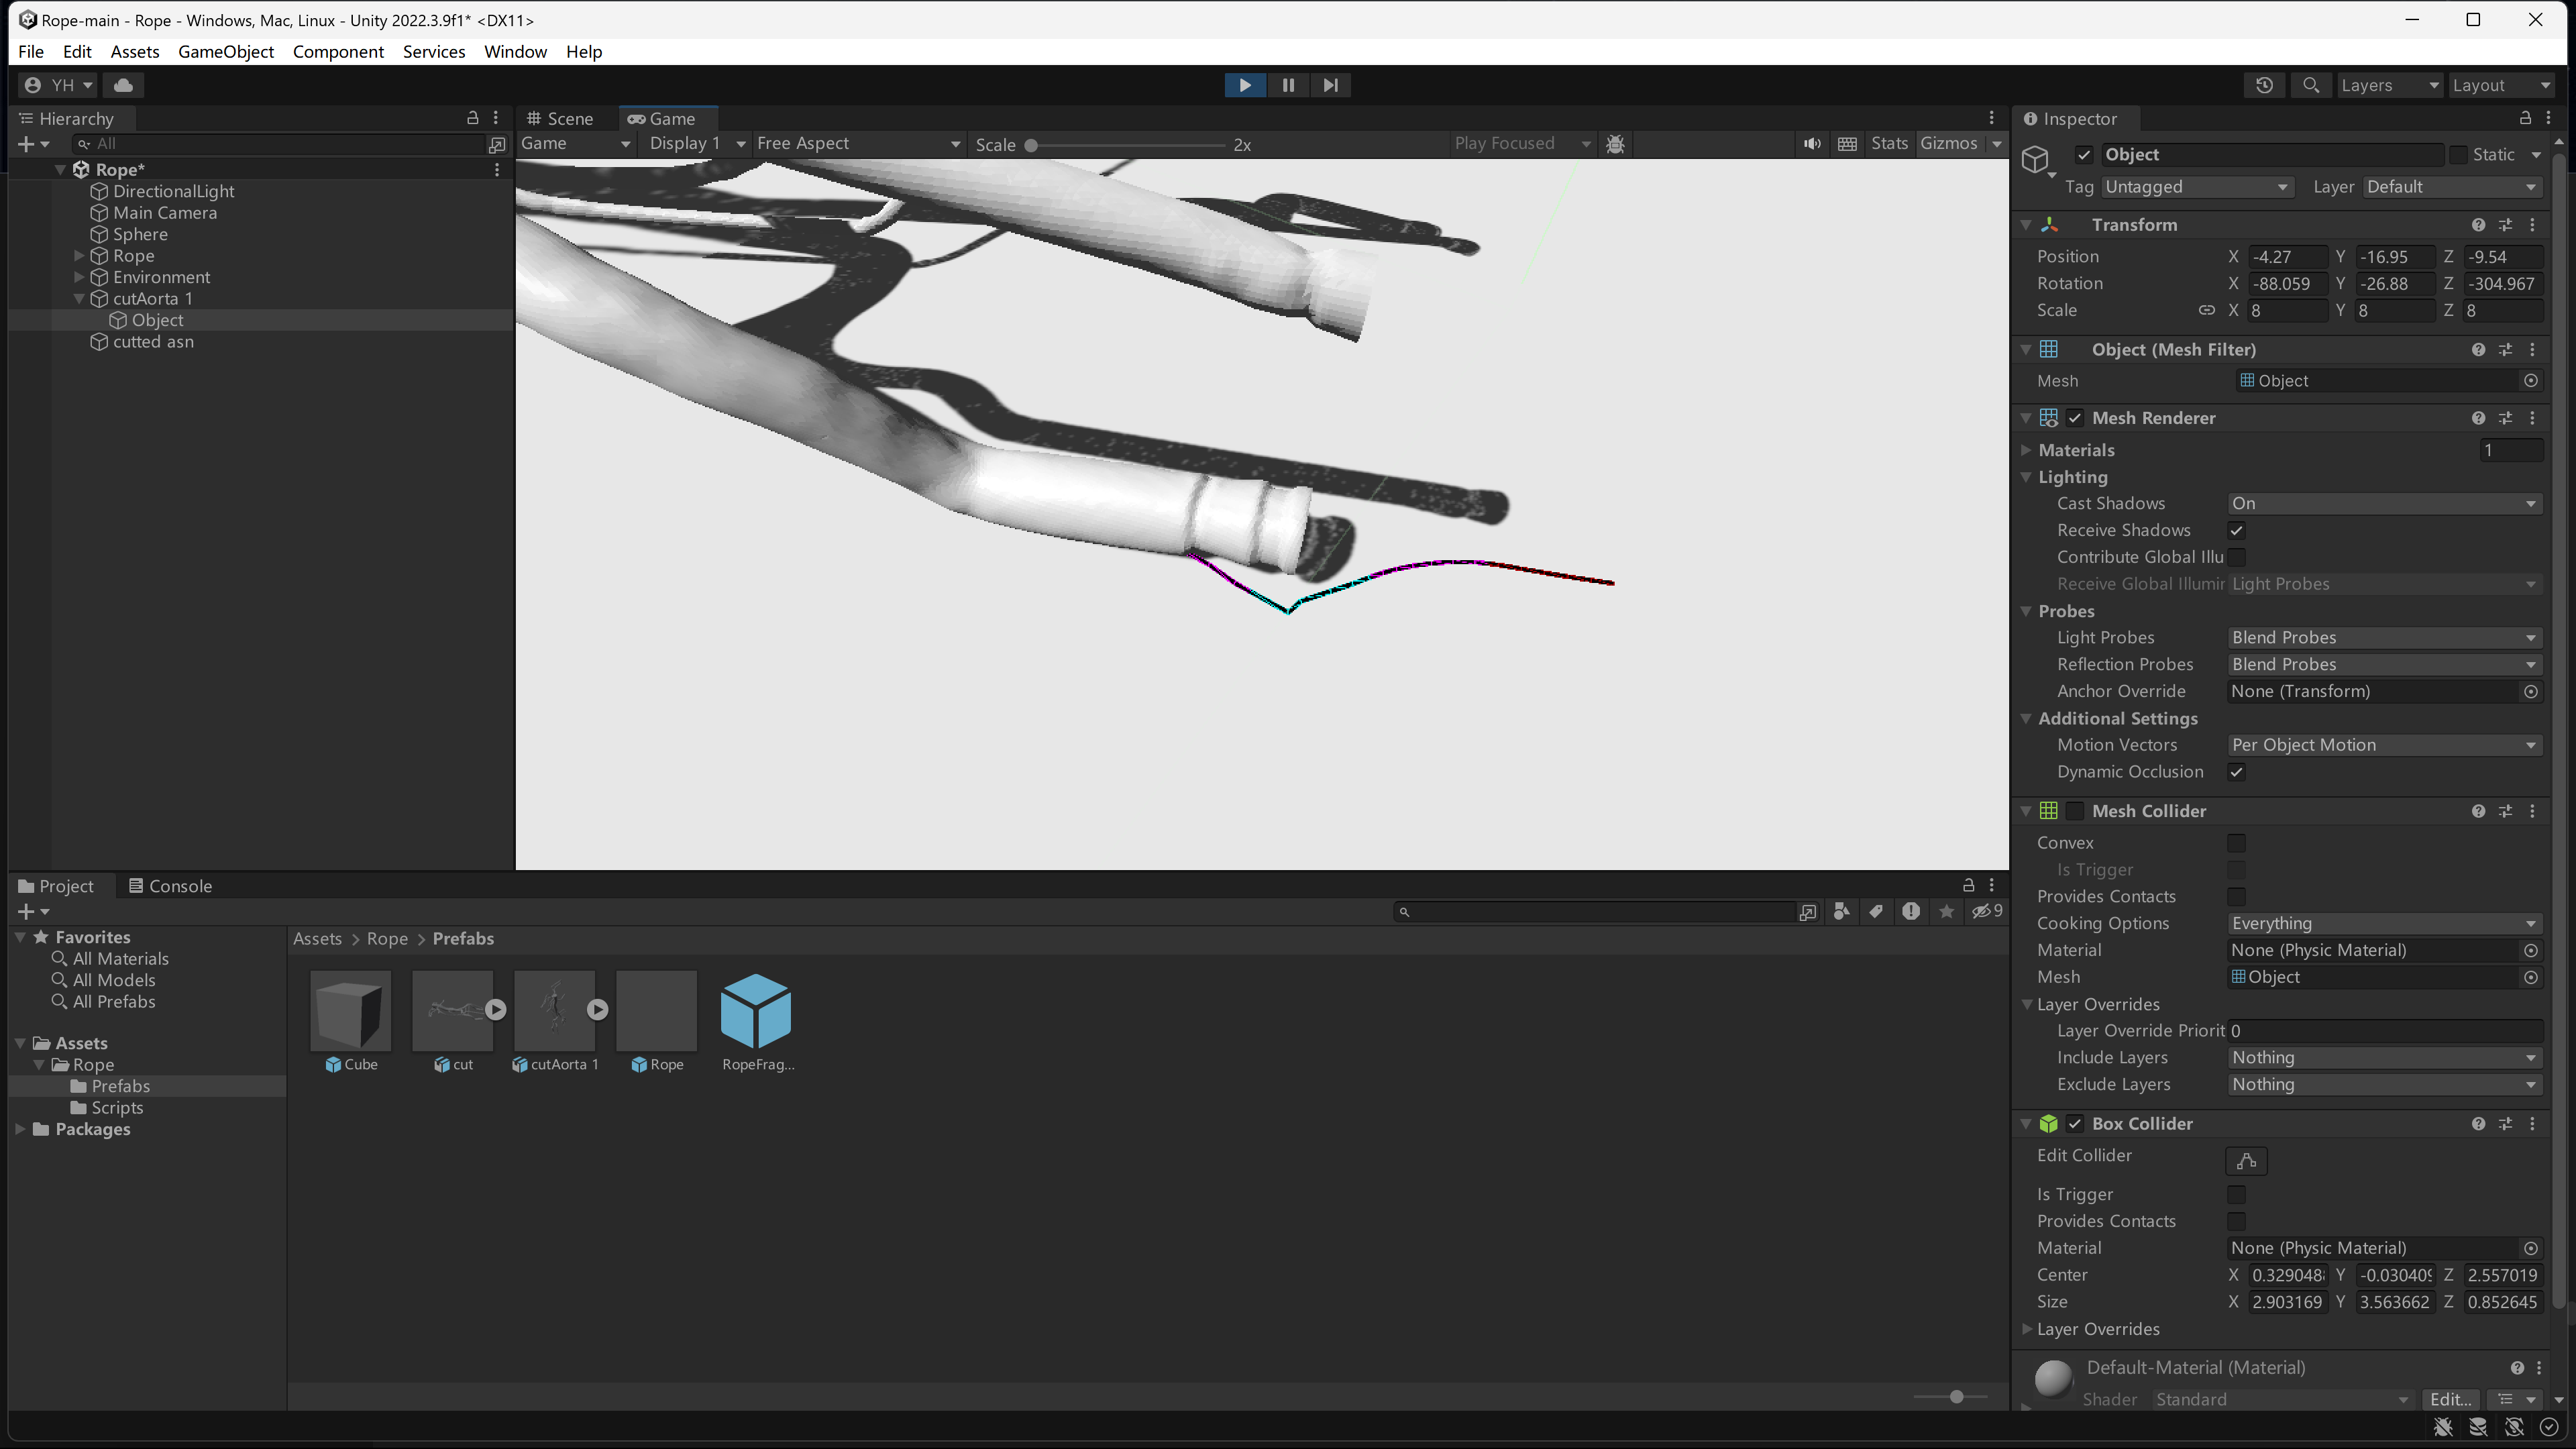
\includegraphics[width=0.8\textwidth]{with box.png}
            \caption{Using Box Collider}
      \end{figure}
      \begin{figure}[H]
            \centering
            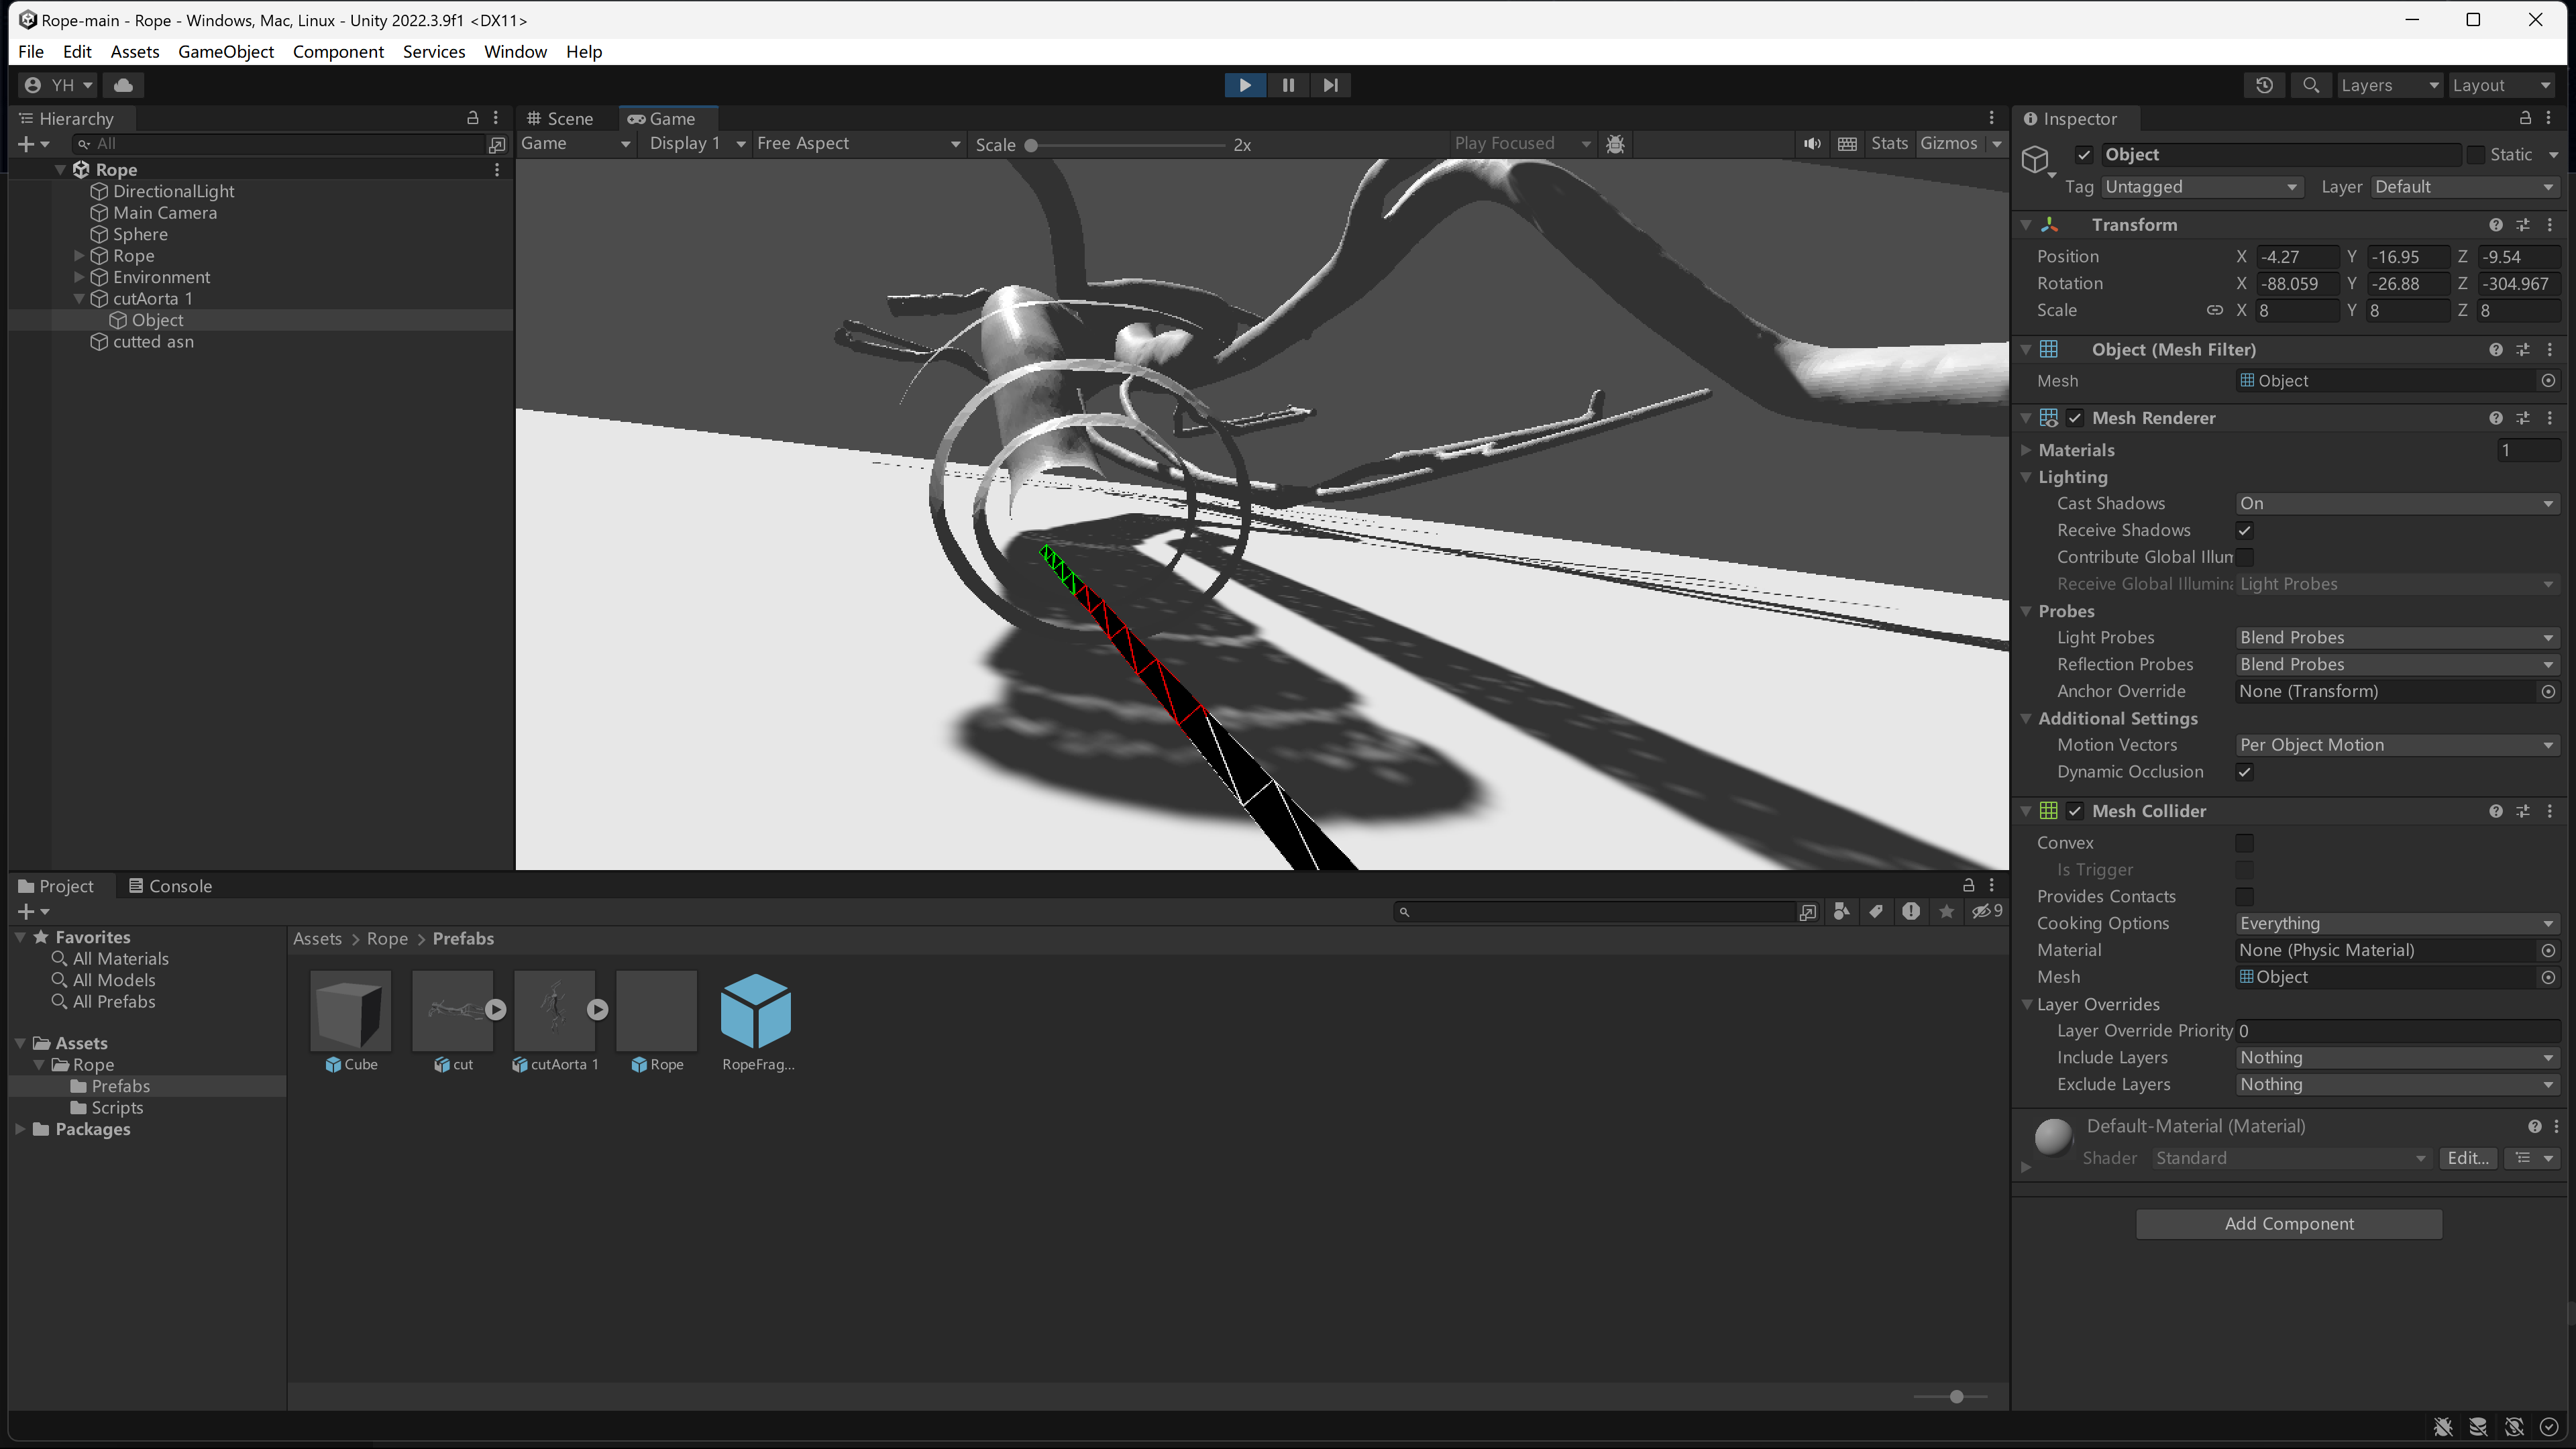
\includegraphics[width=0.8\textwidth]{with mesh.png}
            \caption{Using Mesh Collider}
      \end{figure}
      \begin{figure}[H]
            \centering
            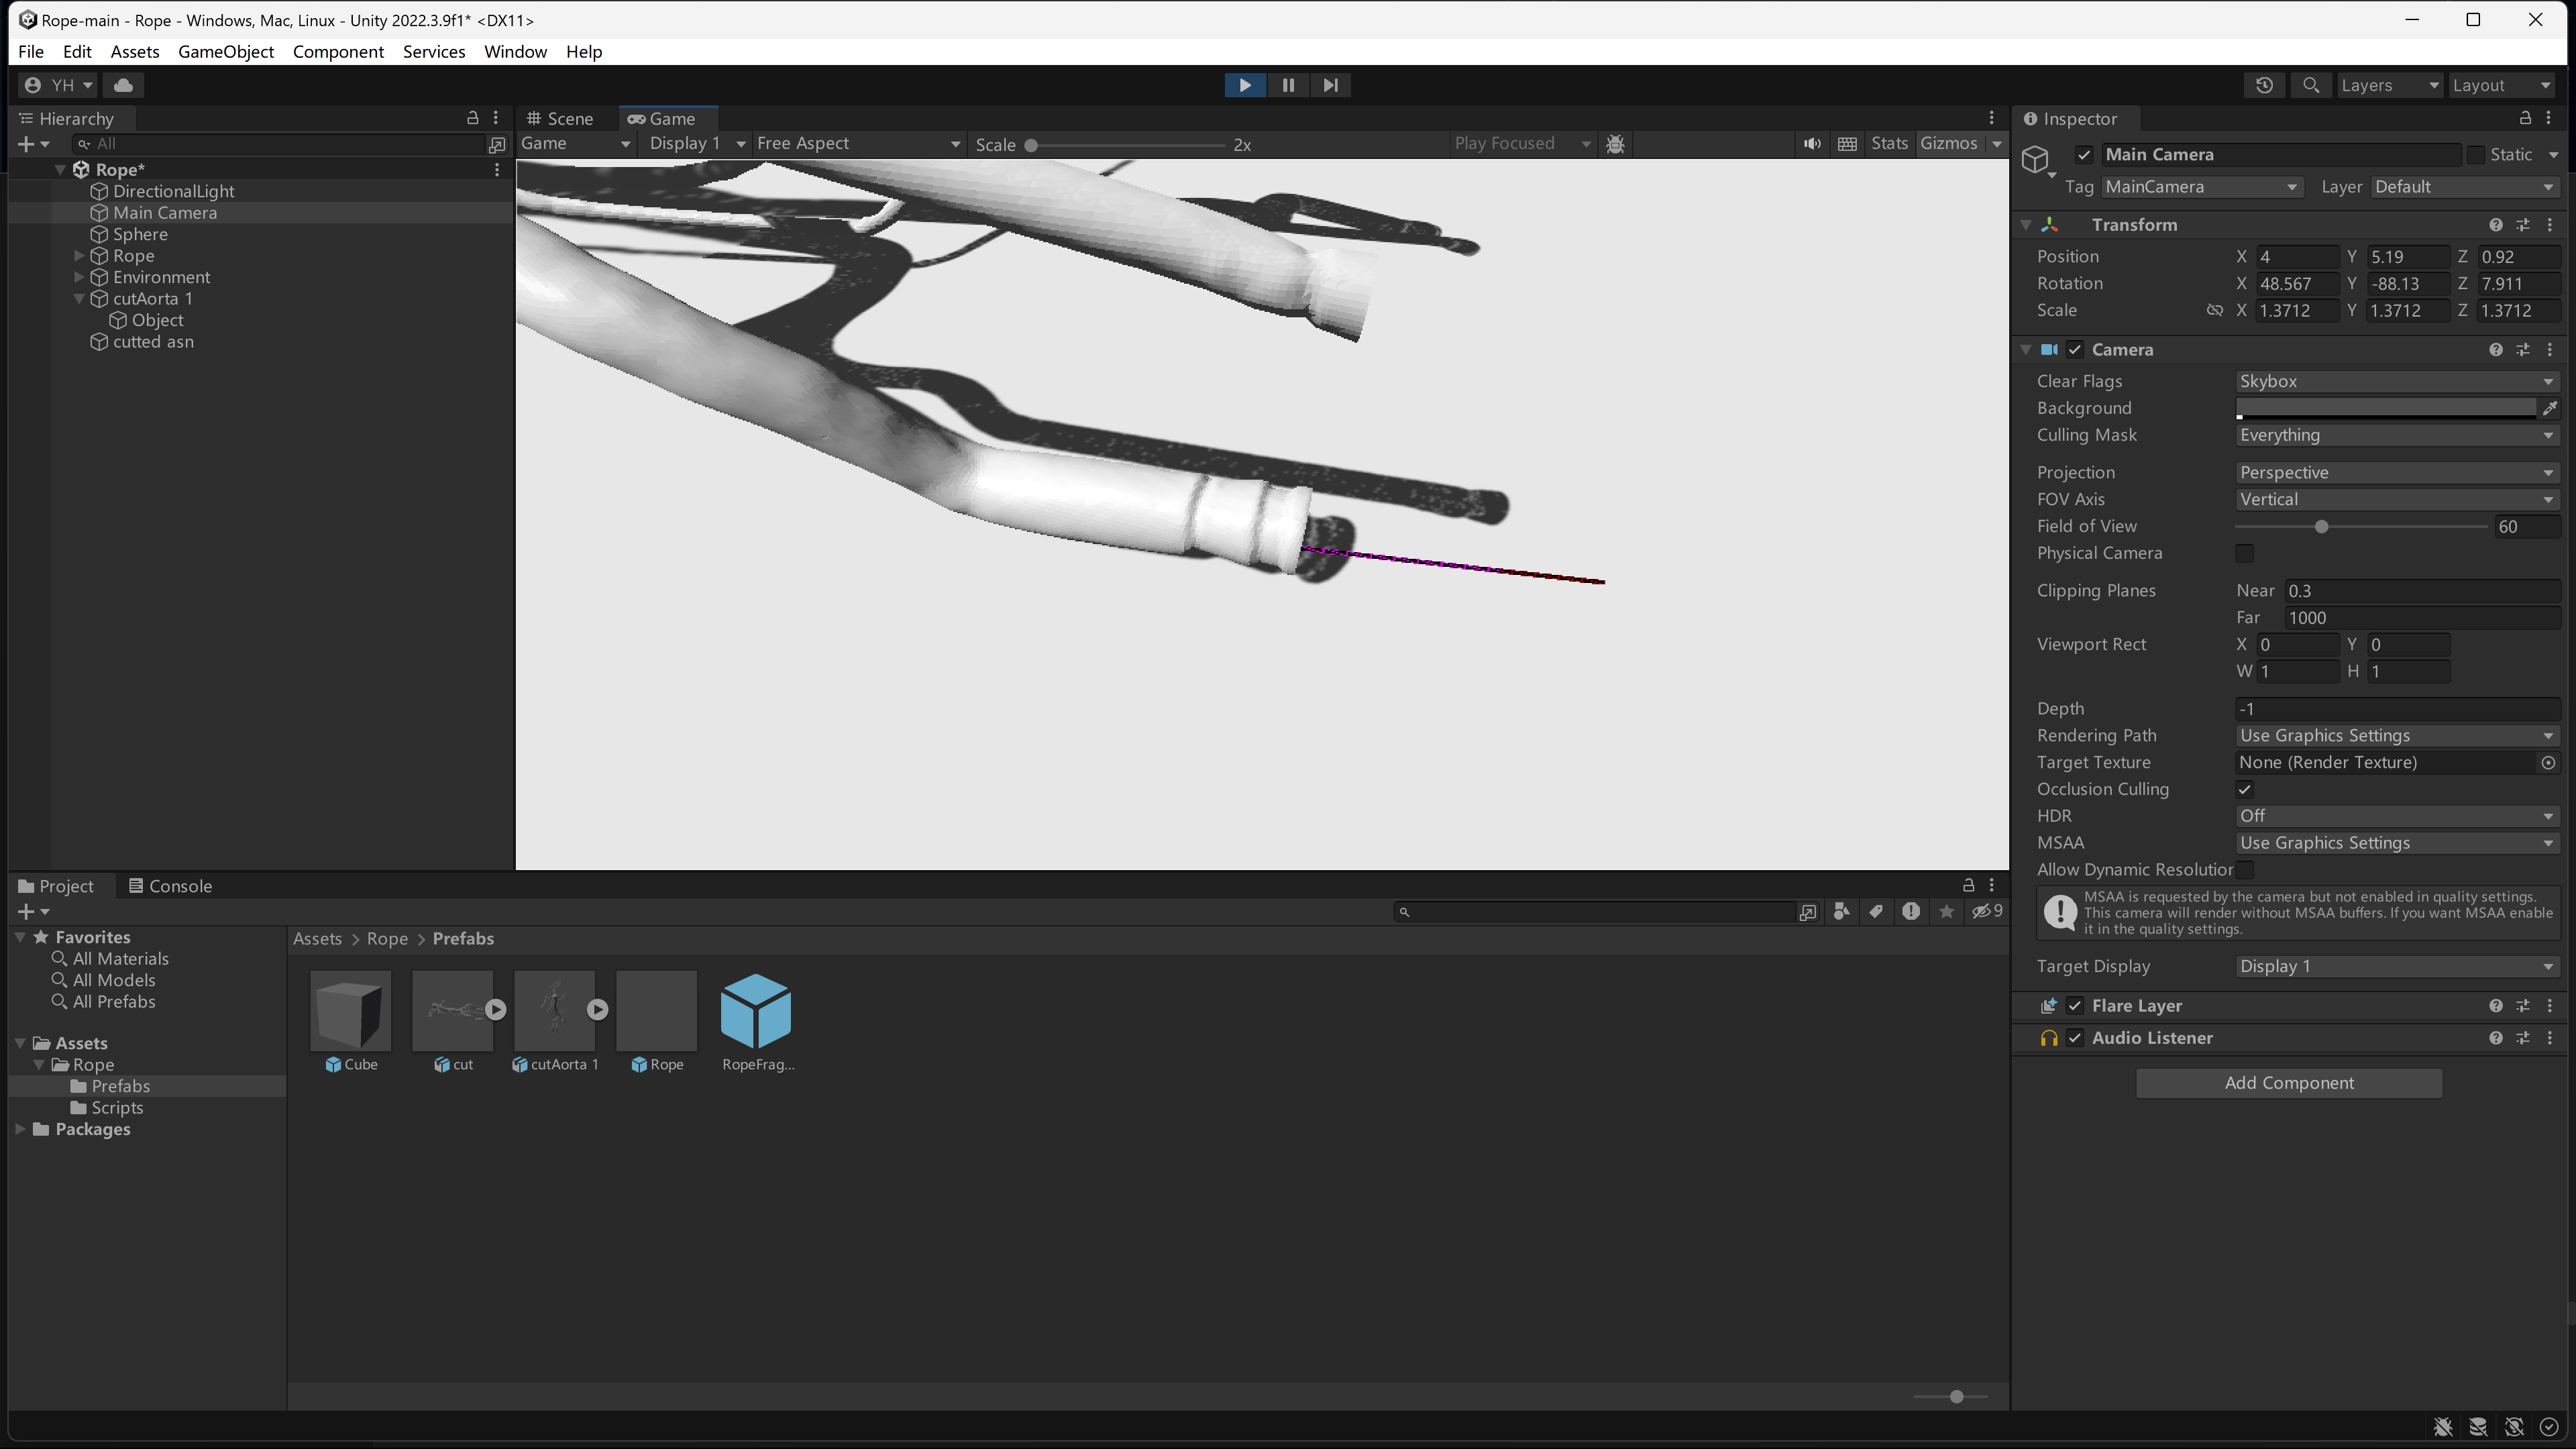
\includegraphics[width=0.8\textwidth]{with mesh1.png}
            \caption{Using Mesh Collider}
      \end{figure}
      Although the basic interaction between Rope and Aorta model is achieved, there are still many problems at this stage. For example, overstretching the Rope and exceeding its elastic limit will cause the Rope to become confused. Moreover, it is not possible to make the Rope deeper into the Aorta at this stage, and the problem of the Rope escaping from the Aorta during the insertion process may also occur.
      \begin{figure}[H]
            \centering
            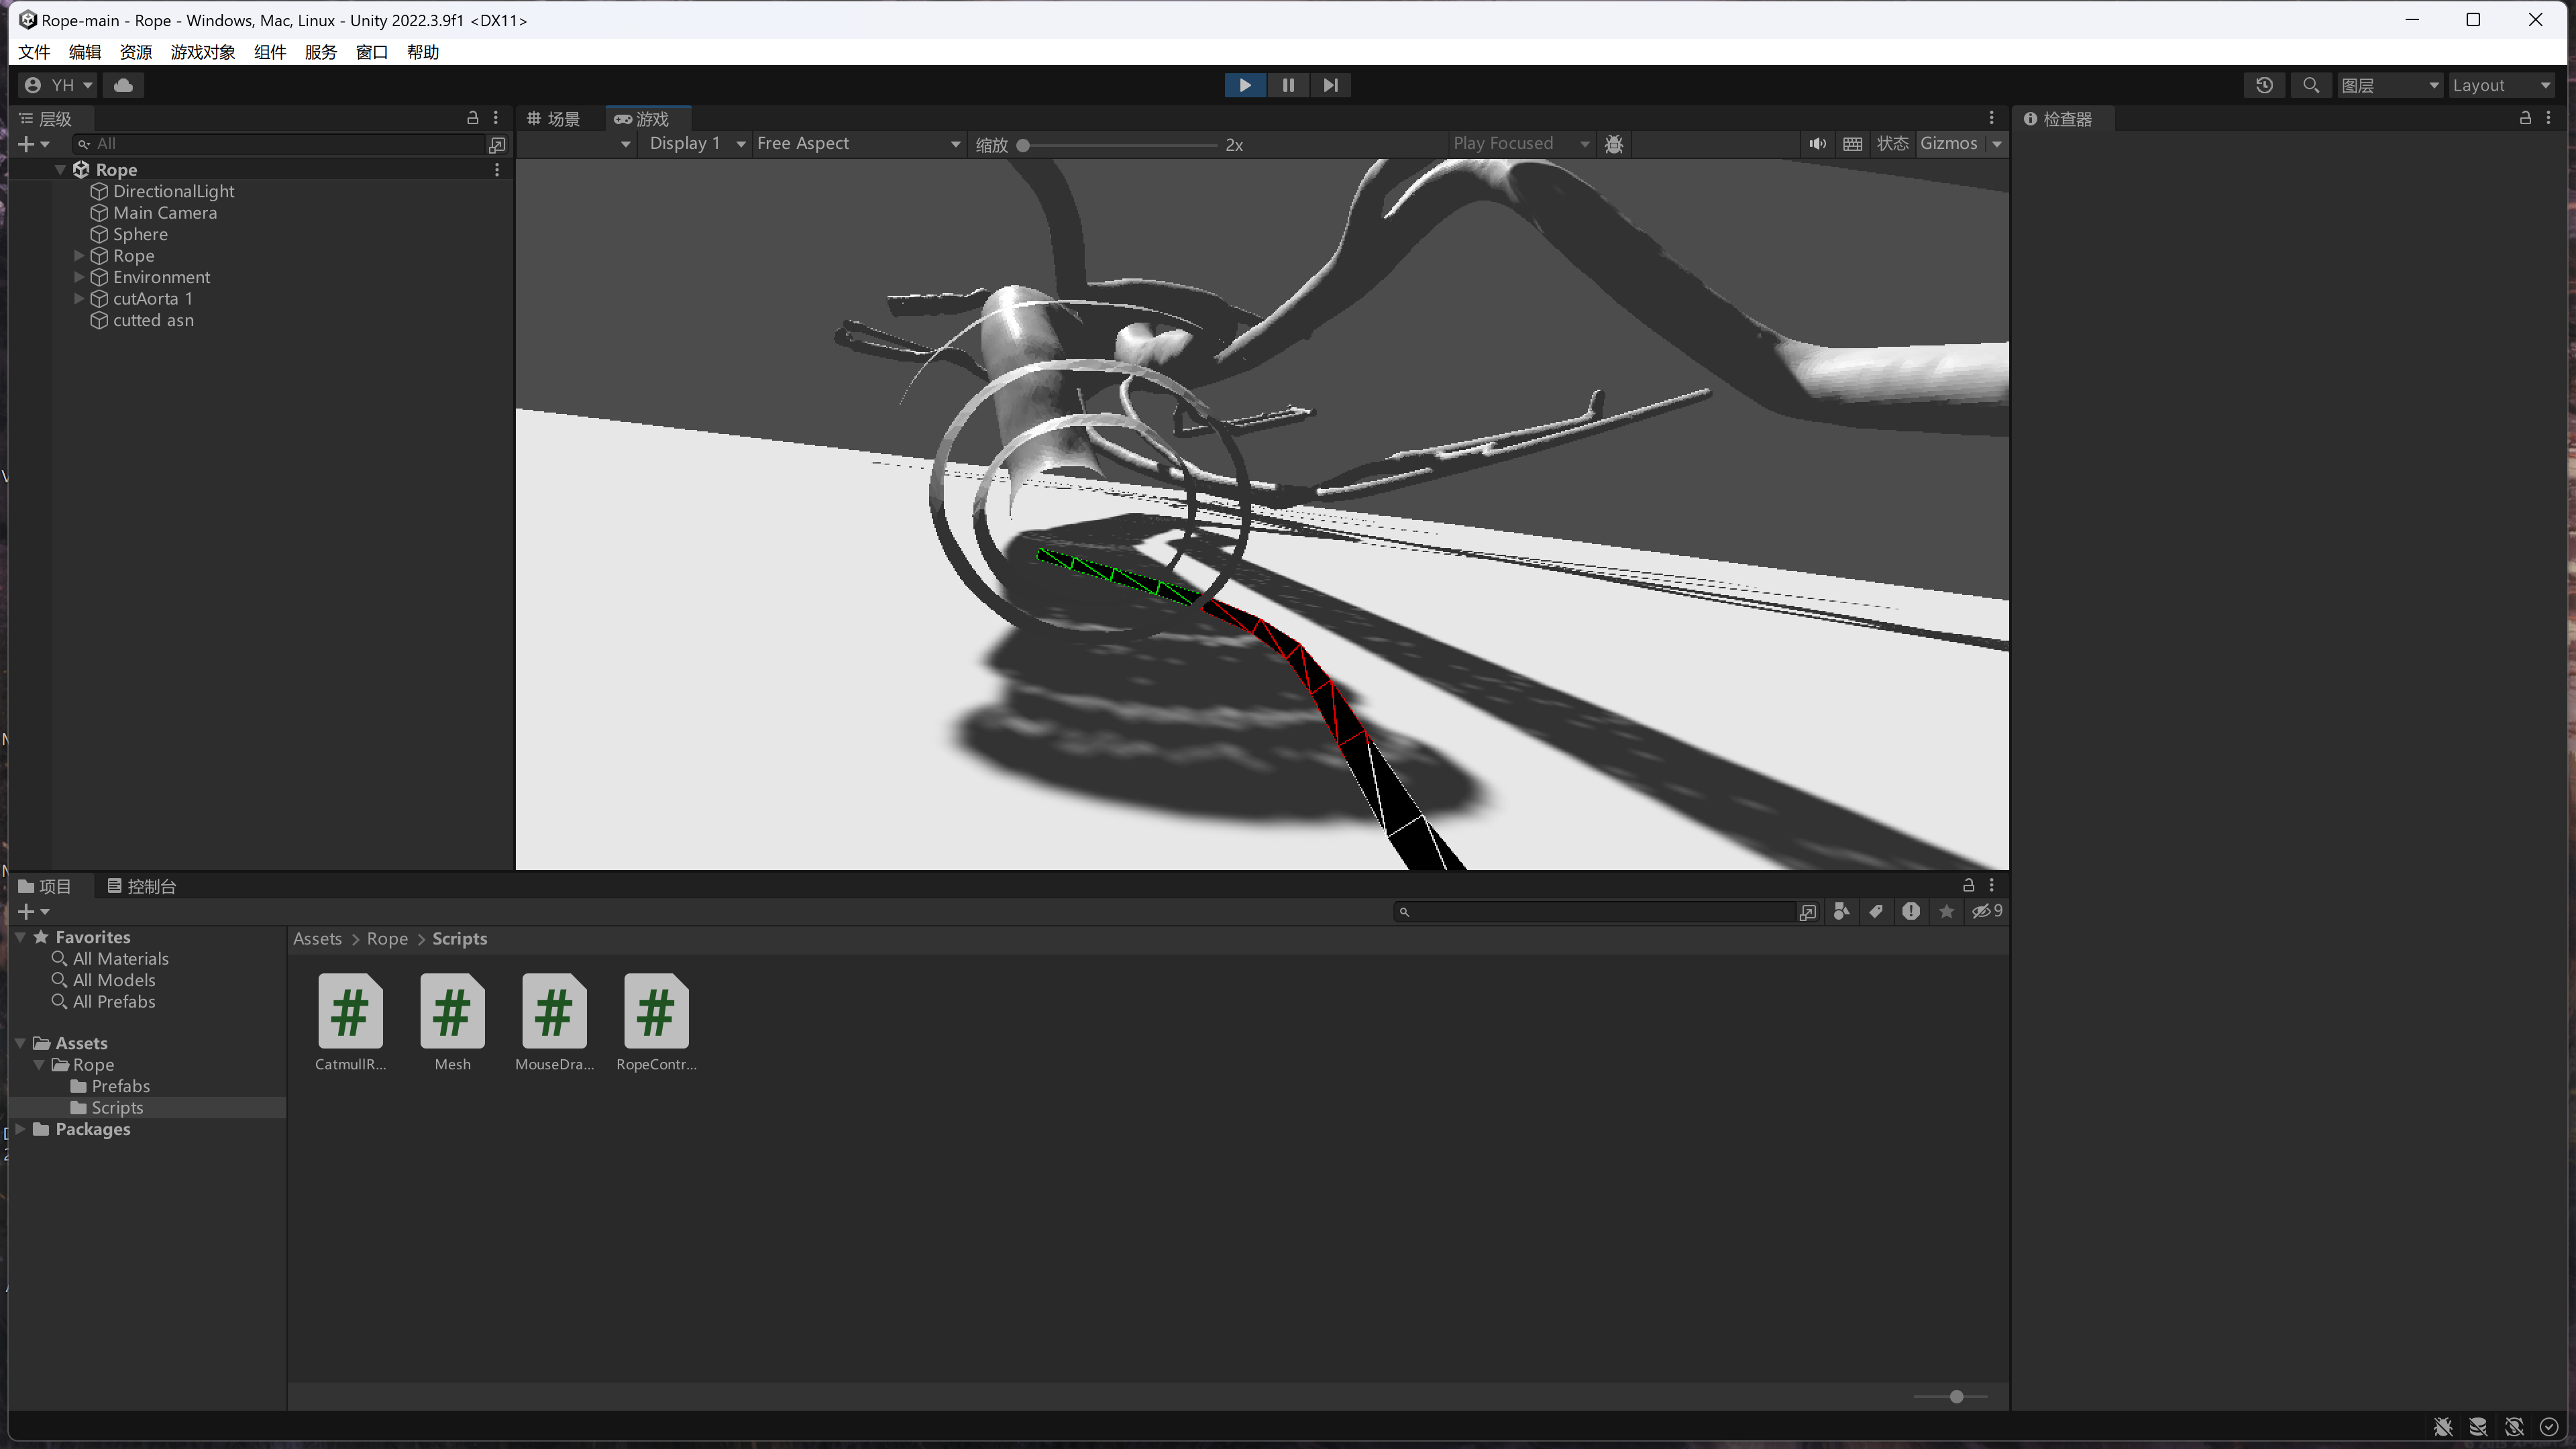
\includegraphics[width=0.8\textwidth]{insert out.png}
            \caption{Rope Insertion Out}
      \end{figure}
      \begin{figure}[H]
            \centering
            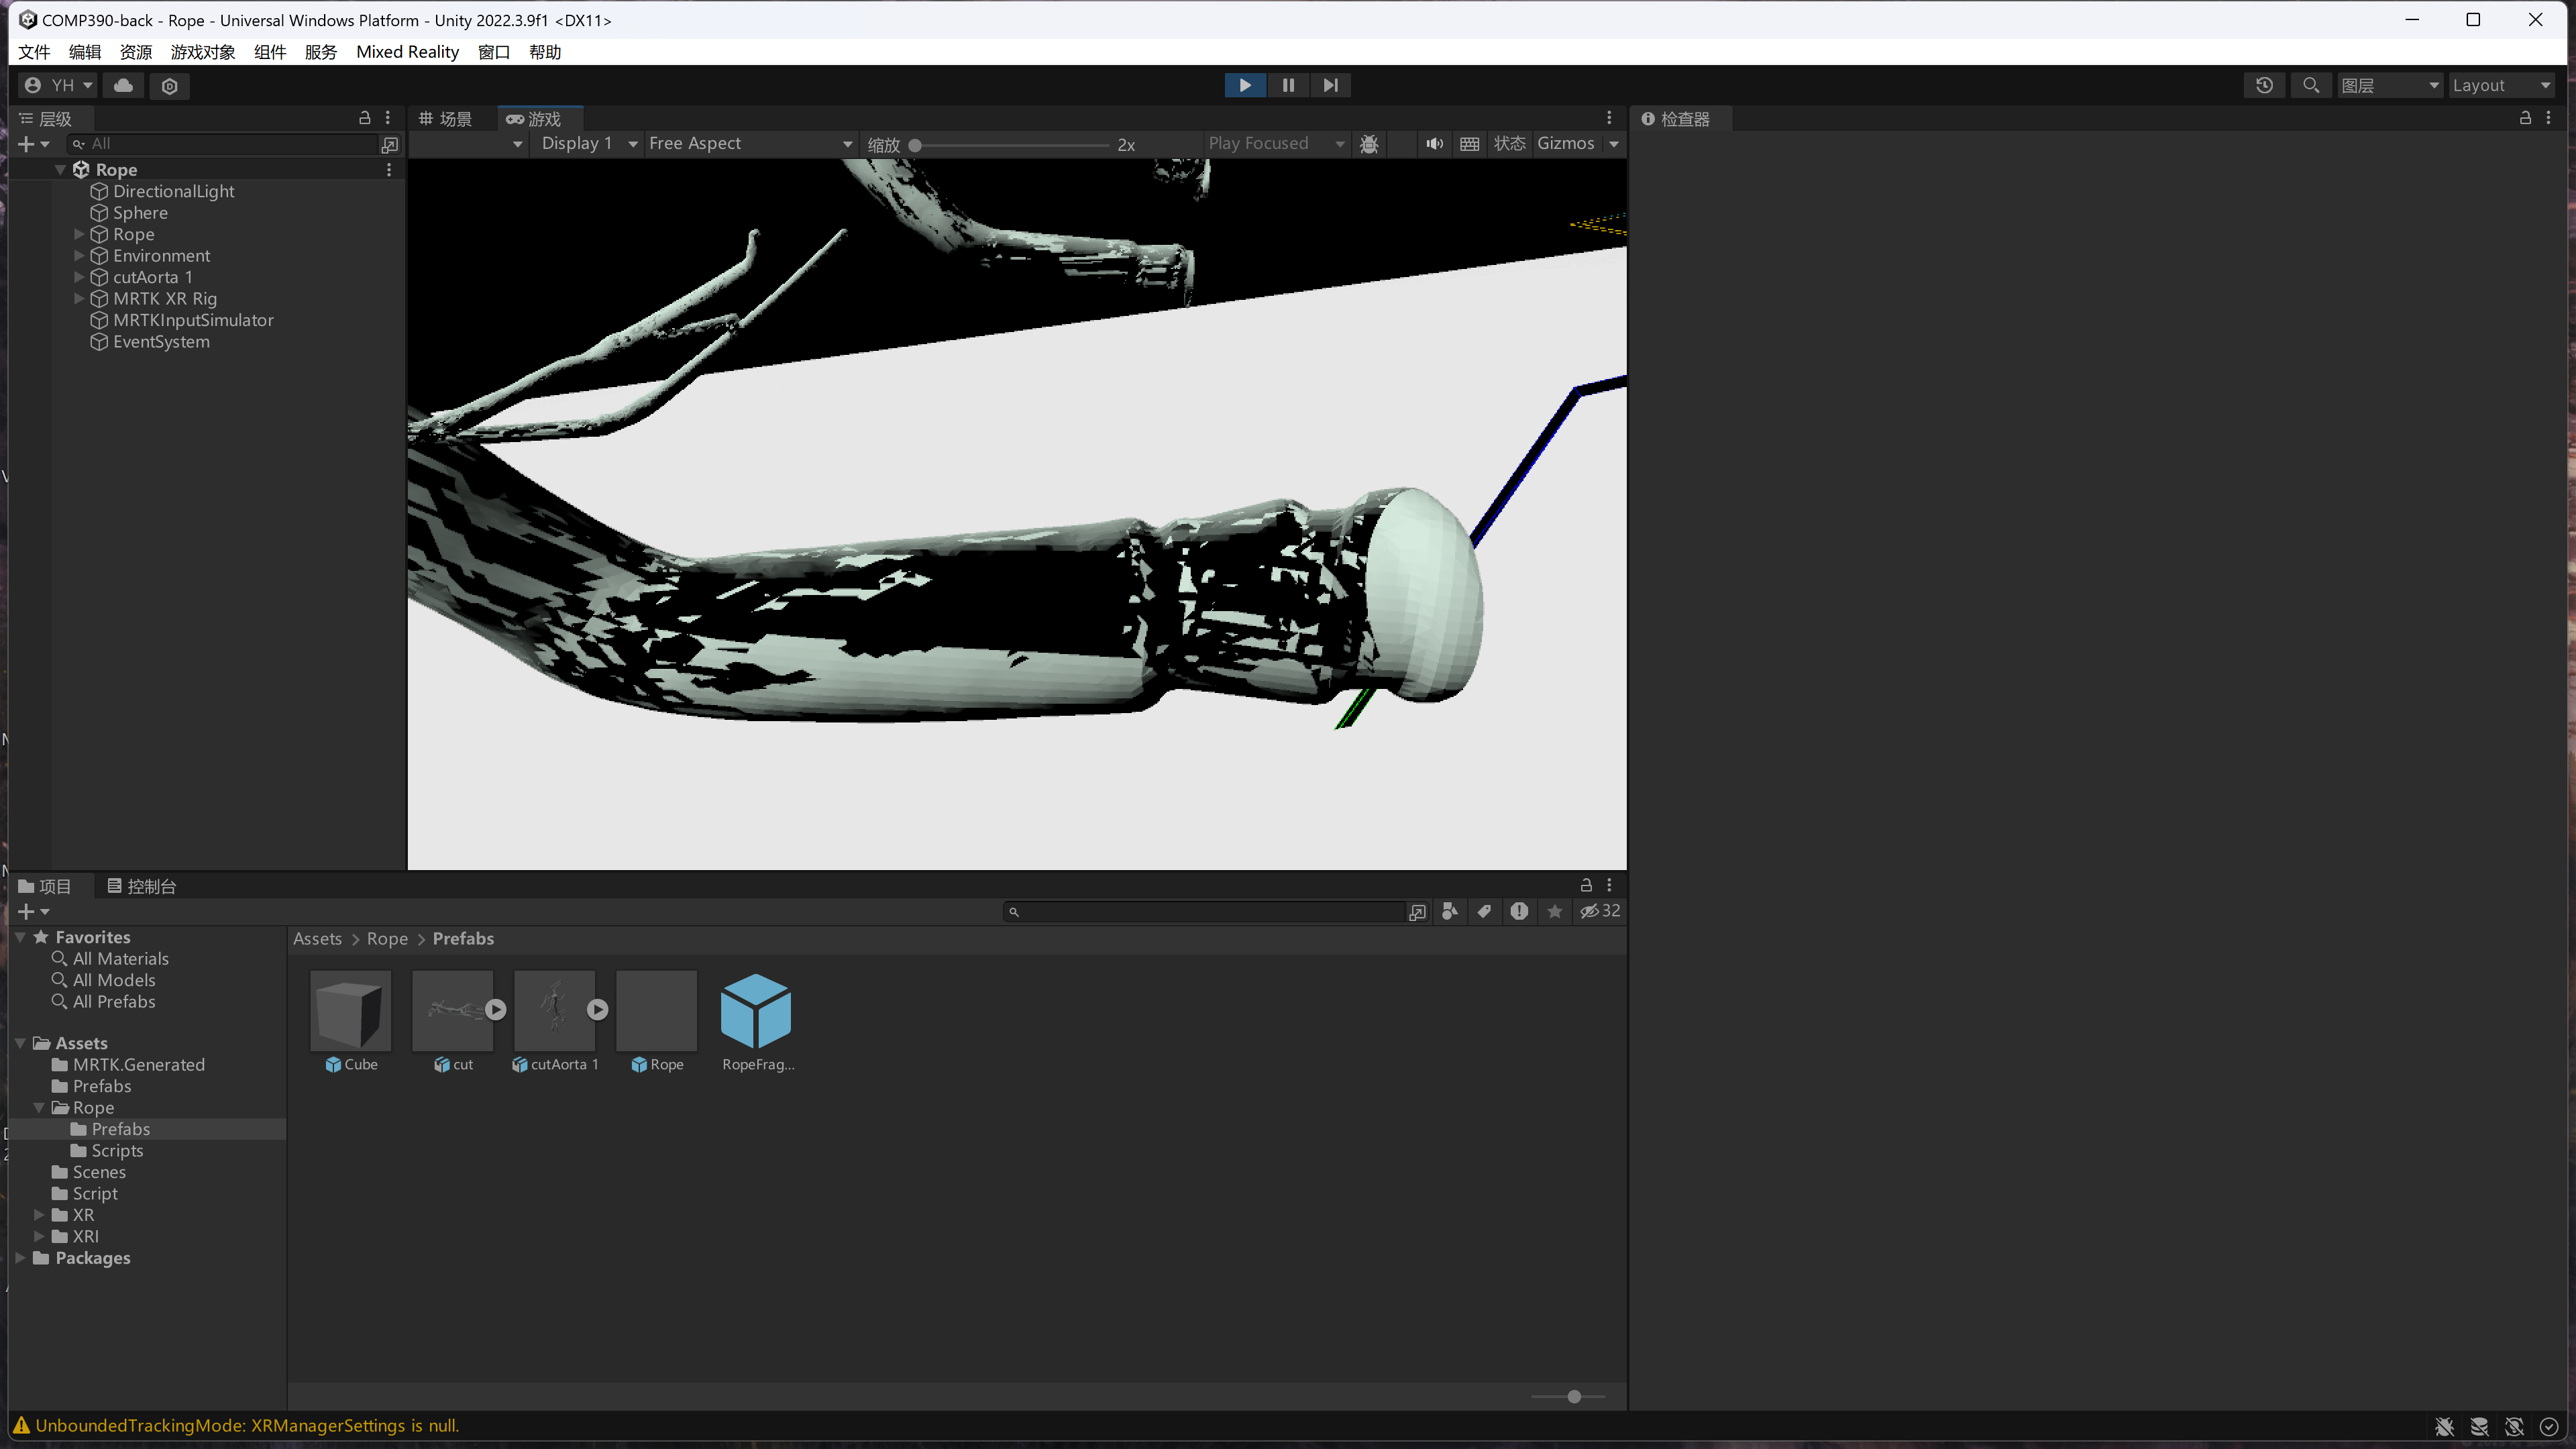
\includegraphics[width=0.8\textwidth]{jittering.png}
            \caption{Rope Jittering}
      \end{figure}
      \item \textbf{Current Stage}
      \\
      After completing all the parts, using the features of the MRTK, it is then possible to simulate with the virtual hand, which can be used to directly control the various postures of the Rope. Similarly, the same effect (except for rotation) can be achieved by using the mouse to click and drag the Rope directly.
      \begin{figure}[H]
            \centering
            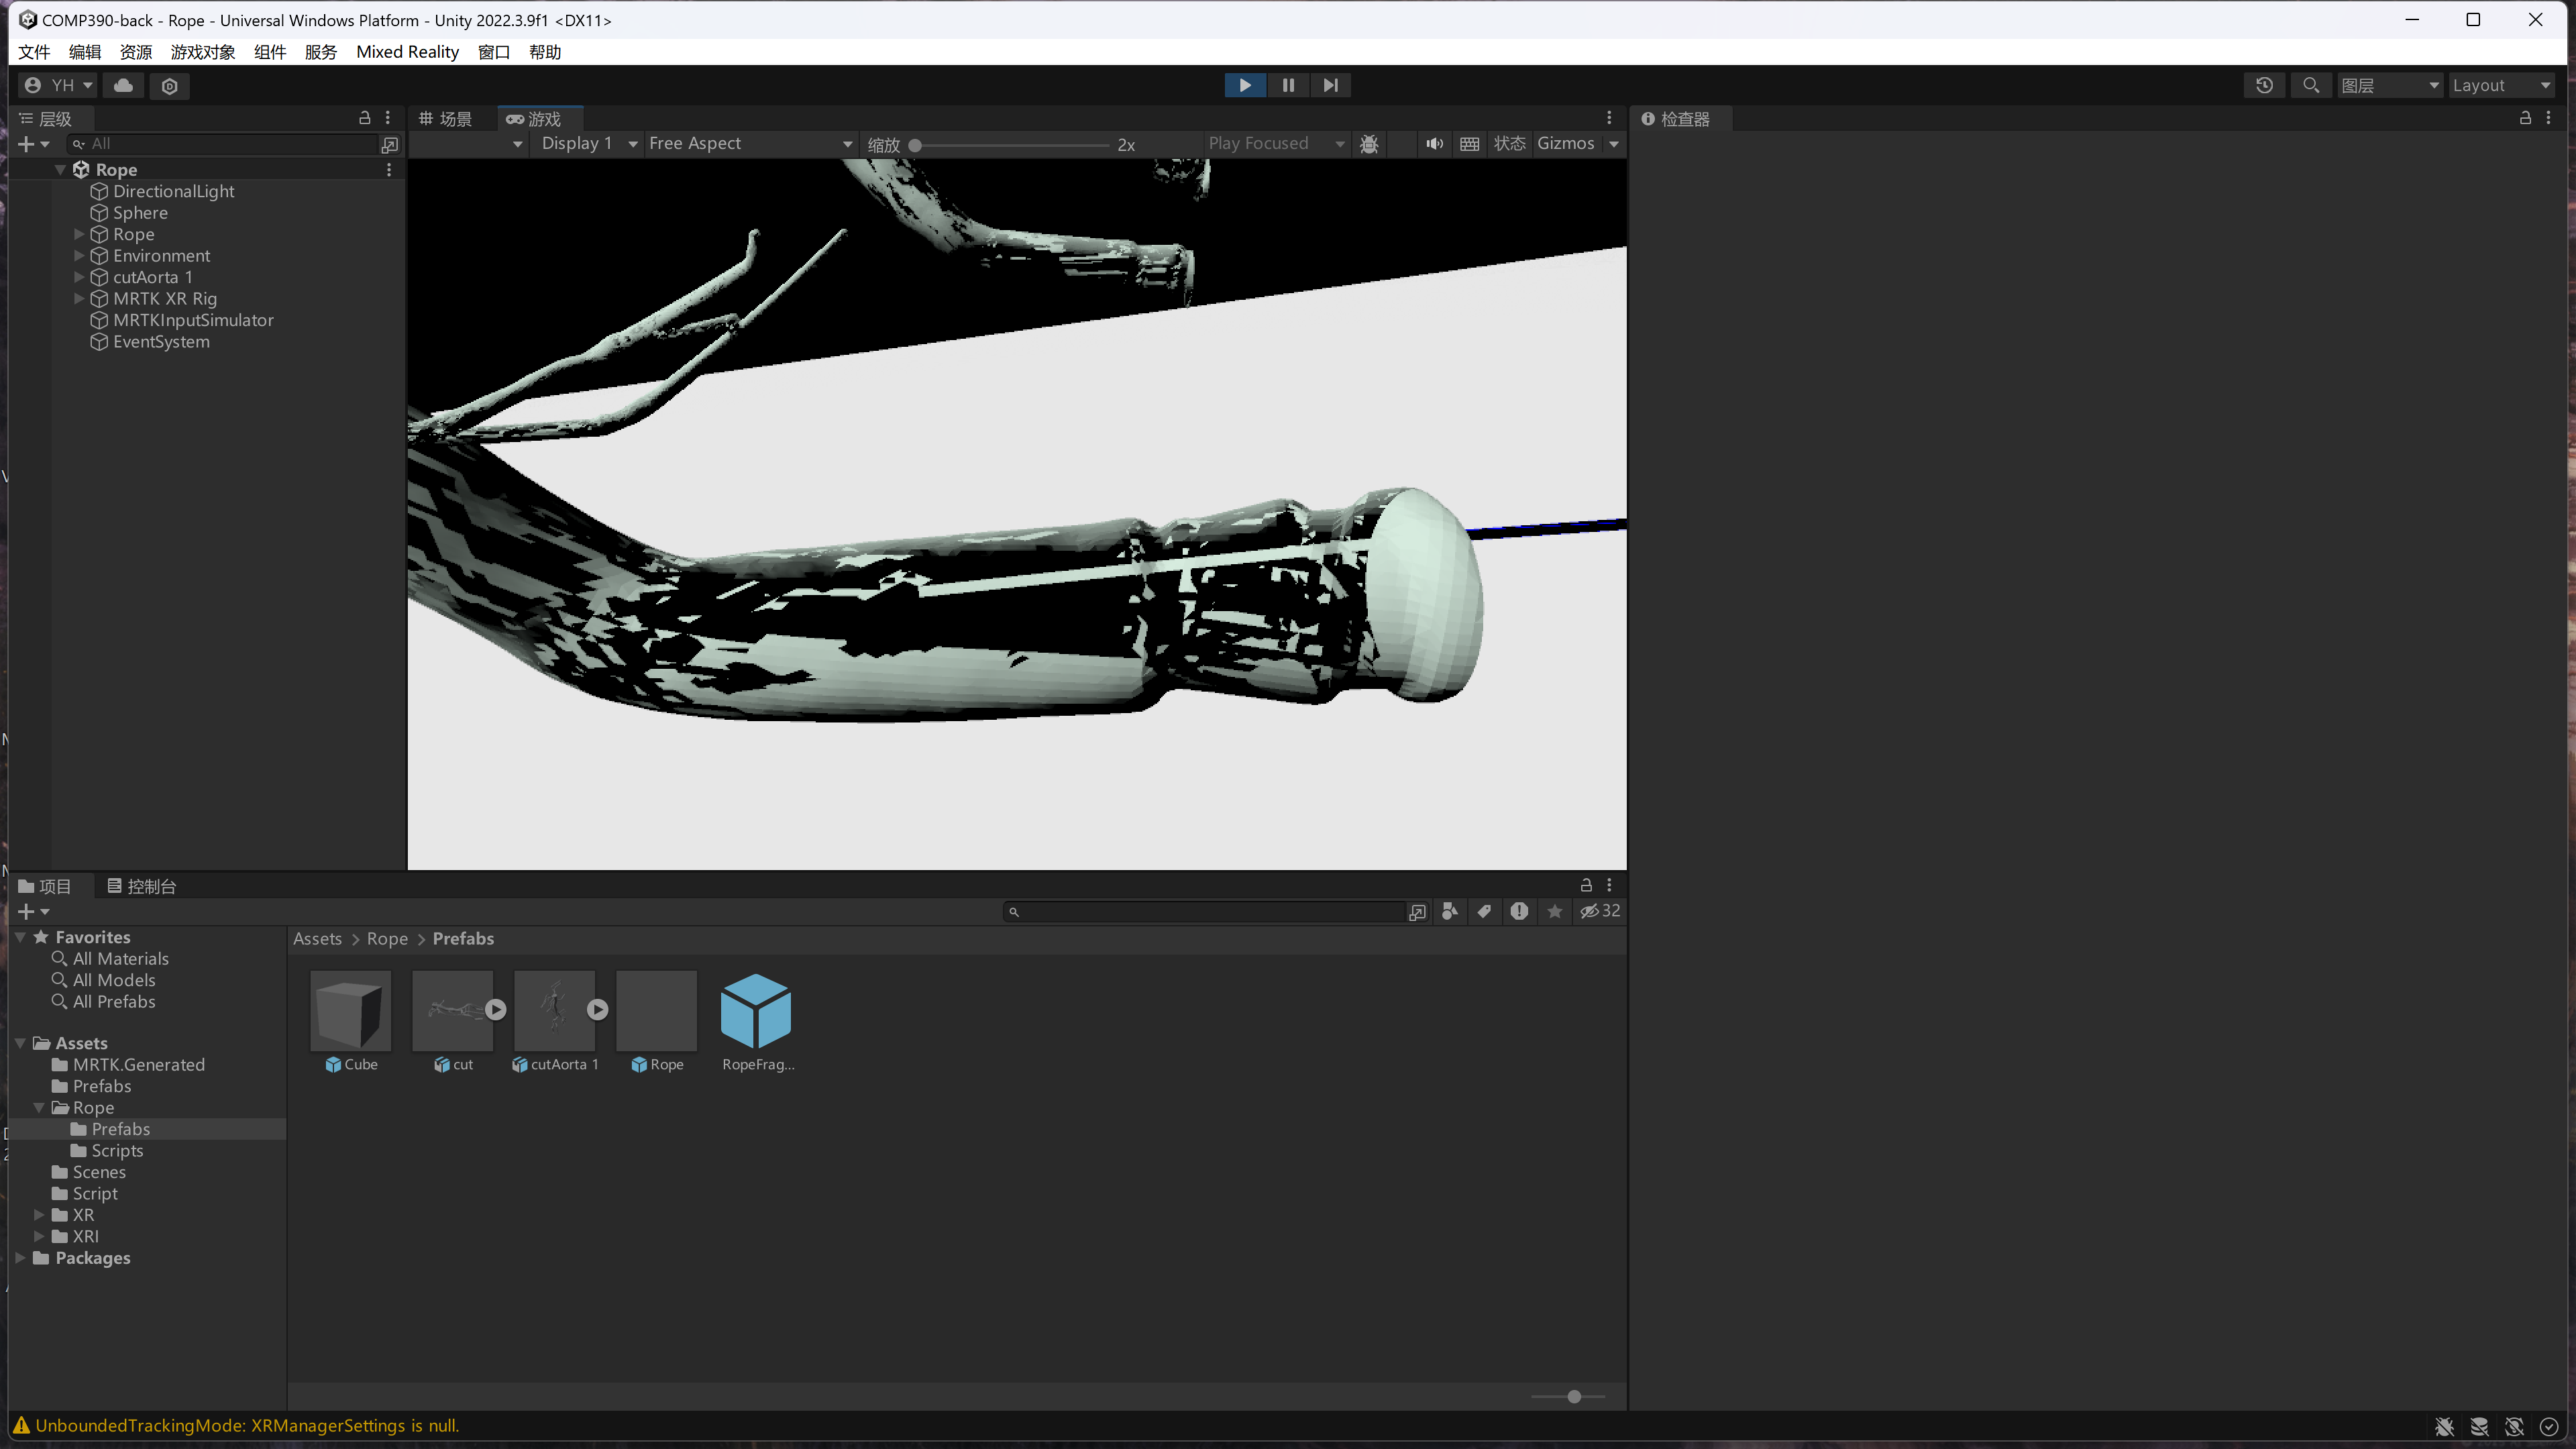
\includegraphics[width=0.8\textwidth]{recent stage.png}
            \caption{Initialize}
      \end{figure}
      \begin{figure}[H]
            \centering
            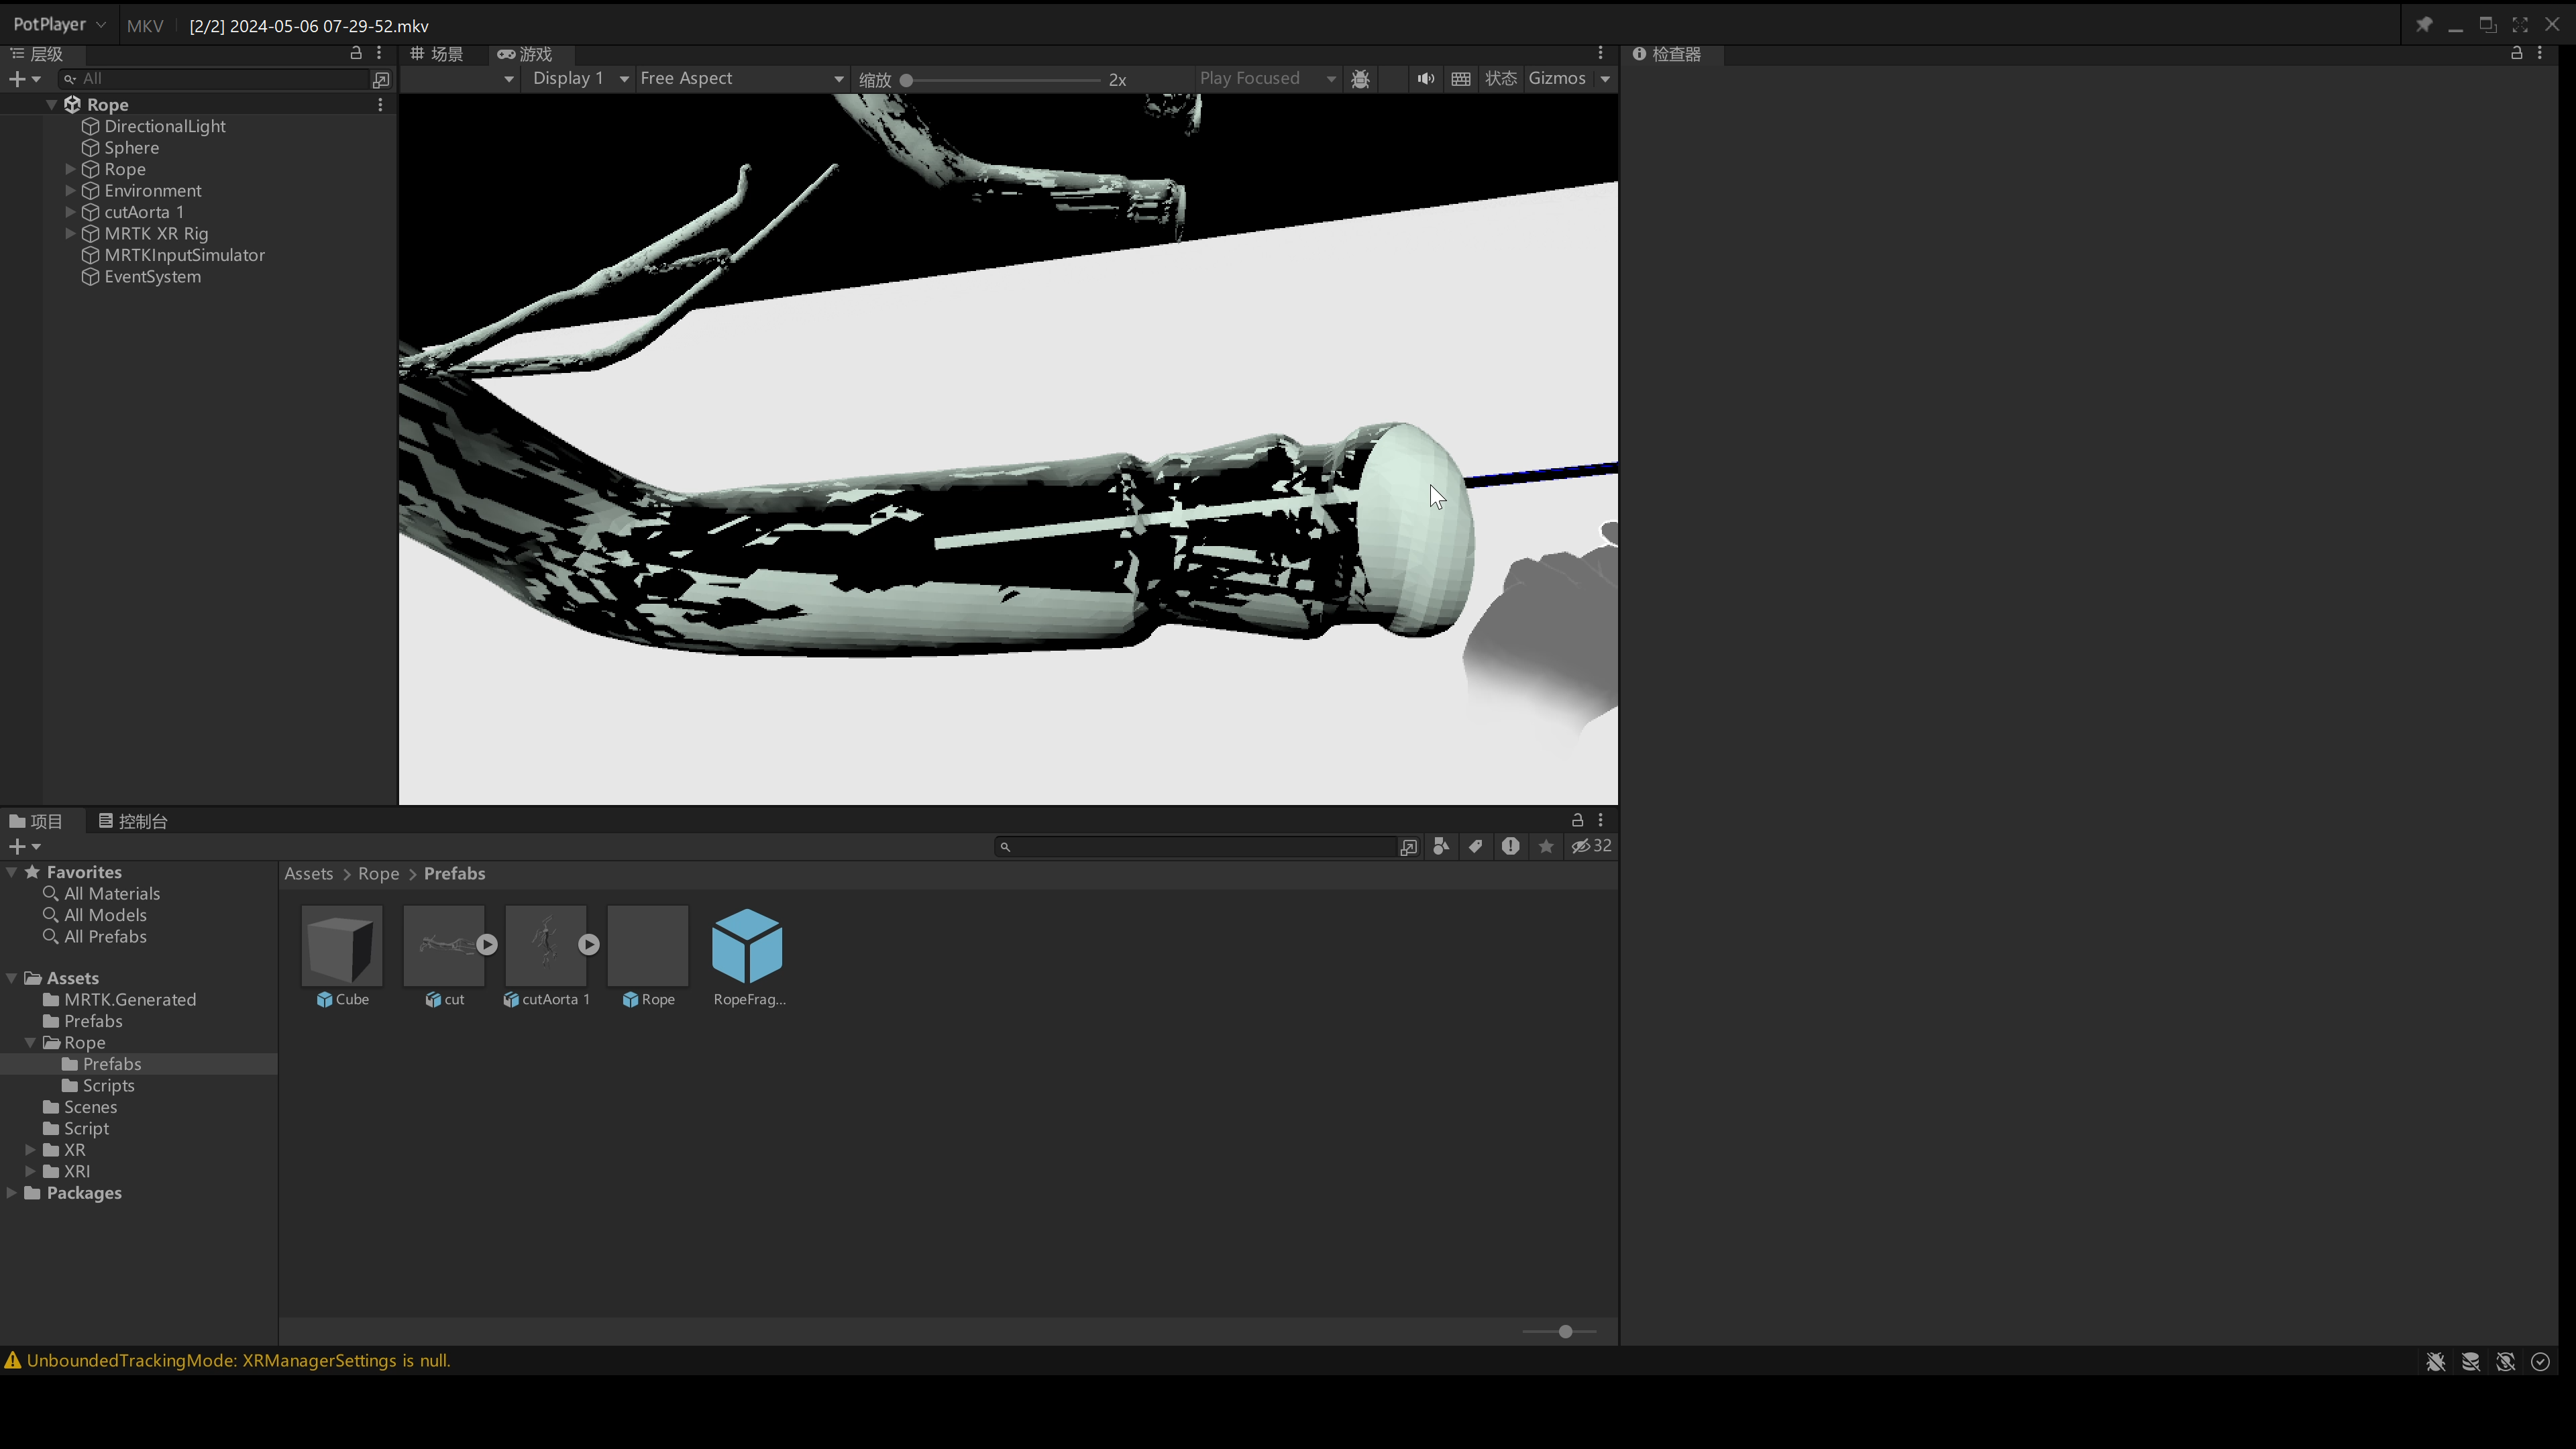
\includegraphics[width=0.8\textwidth]{Insert.png}
            \caption{Insertion}
      \end{figure}
\end{enumerate}


% Testing & Evaluation
\section{Testing \& Evaluation}
\subsection{Part1: Real-world Model Interaction and Tracking}
\subsubsection{Testing}
To test the functionality of Part1, a unit test was created using the \emph{unittest} library\cite{PythonUnittest}.
\begin{itemize}
      \item \textbf{Initialization Test:}
      \\
      The test ensures that the video source and video frame parameters are set correctly when the class is instantiated. This test verifies that the constructor correctly receives and applies the incoming video source and corresponding parameters.
      \item \textbf{Start Test:}
      \\
      Tests if the \emph{start} method starts the timer correctly. By simulating the timer's \emph{isActive} method to return False and re-calling the \emph{start} method, you can check if the timer is set to the normal start frequency.
      \item \textbf{Stop Test:}
      \\
      Tests that the \emph{stop} method effectively stops the timer, and stops the video capture.
      \item \textbf{Update Video Source Controls Test:}
      \\
      Tests that the video source selector and video upload button are set correctly. This includes checking that the video source selector is of type \emph{ QComboBox} and that the upload video button is visible in its initial state.
      \item \textbf{Update View Test:}
      \\
      Detecting whether the screen can be refreshed properly ensures that the model position is instantly refreshed when ArUco marker tracking is performed.
      \item \textbf{Teardown Test:}
      \\
      At the end of the test, ensure that you exit the \emph{QApplication} instance appropriately to avoid memory leaks or other resource hogging issues.  
\end{itemize}
\paragraph{Code for the Testing:}
\begin{minted}[frame=single, linenos=true, fontsize=\footnotesize]{python}
import unittest
from PySide6.QtWidgets import QApplication
from unittest.mock import MagicMock
import sys

# Import your BaseWidget class and other necessary modules
from your_module import BaseWidget, TimestampedVideoSource, VTKOverlayWindow

class TestBaseWidget(unittest.TestCase):
    def setUp(self):
        # Create an QApplication instance because QWidget requires it for initialization.
        self.app = QApplication(sys.argv)
        # Mock the real video source and dimensions
        self.video_source = MagicMock()
        self.dims = (640, 480)
        # Instantiate BaseWidget
        self.widget = BaseWidget(video_source=self.video_source, dims=self.dims)

    def test_initialization(self):
        # Test if initialization correctly sets up the video source and dimensions
        self.assertIsInstance(self.widget.video_source, TimestampedVideoSource)
        self.assertEqual(self.widget.video_source.source, self.video_source)
        self.assertEqual(self.widget.video_source.dims, self.dims)

    def test_start(self):
        # Test if the timer starts running after calling the start method
        self.widget.timer.isActive = MagicMock(return_value=False)
        self.widget.start()
        self.widget.timer.start.assert_called_once_with(1000.0 / self.widget.update_rate)

    def test_stop(self):
        # Test if the timer stops after calling the stop method
        self.widget.stop()
        self.assertTrue(self.widget.timer.stop.called)

    def test_update_video_source_controls(self):
        # Test if video source controls are set up correctly
        self.assertIsInstance(self.widget.video_source_selector, QComboBox)
        self.assertTrue(self.widget.upload_video_button.isVisible())

    def test_update_view(self):
        # Ensure that update_view throws NotImplementedError
        with self.assertRaises(NotImplementedError):
            self.widget.update_view()

    def tearDown(self):
        # Properly quit the QApplication instance
        self.app.quit()

if __name__ == '__main__':
    unittest.main()
\end{minted}
\subsubsection{Evaluation}
\begin{itemize}
      \item \textbf{Functional Evaluation:}
      \\
      The part achieves features such as real-time video capture, model overlays and ArUco marker tracking that were requested during the design phase. Additional features such as model colour modification, video source switching, ArUco parameter setting and ArUco generator have been added. The part has been successfully implemented and tested, and the functionality is stable and reliable.
      \item \textbf{Performance Evaluation:}
      \\
      After performance evaluation, this section can be used normally in most cases, but if the uploaded video frame rate is too high, the resolution is too high or the video is too large, it may cause the uploaded video interface to lag. In this case it may also cause video stuttering and poor tracking within the application interface.
      \item \textbf{User Experience Evaluation:}
      \\
      The app's application interface is simple and logical, with relatively easy instructions and operations for various functions. However, when deploying the application, you may need to install the required open source libraries and configure the environment.
      \item \textbf{Maintainability and scalability evaluation:}
      \\
      The application was developed using Pyside 6 for the front-end, and individual features were added as widgets with a high degree of maintainability and extensibility. The core functions of video capture, model tracking, and video source switching were split and organised into multiple classes for easy maintenance and upgrading afterwards.
      \end{itemize}
\subsection{Part2: Endovascular Intervention Simulation}
\subsubsection{Testing}
To test the functionality of Part2, a unit test was created using the \emph{Nunit} library\cite{NUnit2023}.
\begin{enumerate}
      \item \textbf{Test environment setup and cleanup:}
            \begin{itemize}
                  \item \textbf{SetUp method:}
                  \\
                  Before starting a new test using \emph{Nunit}, first build the test environment using the \emph{SetUp } method first. This creates a new GameObject object and adds the RopeController component to it for use in subsequent tests.
                  \item \textbf{TearDown method:}
                  \\
                  Clean up the test environment by executing the \emph{TearDown} method after each test is completed. This destroys the GameObject object created in the \emph{SetUp } method and ensures that the environment is reset after each test is run, avoiding the need for different tests to interact with each other.
            \end{itemize}
            \item \textbf{Test Case Description:}
            \begin{itemize}
                  \item \textbf{Testing the correct number of segments:}
                  \\
                  This verifies that the specified number of fragments are created correctly when the \emph{Start} method in \emph{RopeController} is called.This test checks that the fragment array is the preset length of 80 to ensure that the fragments are initialised correctly.
                  \item \textbf{Test the correctness of the segment position:}
                  \\
                  This test further checks that the position of each fragment is set correctly after the \emph{Start } method is called. This test ensures that each fragment is placed in the correct position by verifying the incremental position of each fragment on the z-axis (the default is 0.25 units of length per interval).
                  \item \textbf{Testing LineRenderer position updates:}
                  \\
                  After executing the \emph{LateUpdate} method, it will be verified that the position array of the \emph{LineRenderer} component has been updated and matches the current position of the fragment. This test checks that visual elements, such as line rendering, respond correctly to background data changes.
            \end{itemize}
      \end{enumerate}
\begin{minted}[frame=single, linenos=true, fontsize=\footnotesize]{Java}
using NUnit.Framework;
using UnityEngine;
using UnityEngine.TestTools;

namespace Rope.Tests
{
    public class RopeControllerTests
    {
        private RopeController _ropeController;
        private GameObject _ropeControllerGameObject;

        [SetUp]
        public void SetUp()
        {
            _ropeControllerGameObject = new GameObject();
            _ropeController = _ropeControllerGameObject.AddComponent<RopeController>();
        }

        [TearDown]
        public void TearDown()
        {
            Object.Destroy(_ropeControllerGameObject);
        }

        [Test]
        public void Start_WithValidParameters_CreatesCorrectNumberOfFragments()
        {
            _ropeController.Start();

            Assert.AreEqual(80, _ropeController.fragments.Length);
        }

        [Test]
        public void Start_WithValidParameters_CreatesFragmentsWithCorrectPositions()
        {
            _ropeController.Start();

            for (int i = 0; i < _ropeController.fragments.Length; i++)
            {
                Assert.AreEqual(i * 0.25f, 
                _ropeController.fragments[i].transform.position.z);
            }
        }

        [Test]
        public void LateUpdate_WithValidParameters_UpdatesLineRendererPositions()
        {
            _ropeController.Start();
            _ropeController.LateUpdate();

            var lineRenderer = _ropeController.GetComponent<LineRenderer>();

            for (int i = 0; i < _ropeController.fragments.Length; i++)
            {
                Assert.AreEqual(_ropeController.fragments[i].transform.position, 
                lineRenderer.GetPosition(i));
            }
        }
    }
}
\end{minted}
\subsubsection{Evaluation}
\begin{itemize}
      \item \textbf{Functional Evaluation:}
      \\
      This section implements the most basic functional requirements of the design phase of the project, such as the main simulation processes of Endovascular Intervention, the methods of interaction and manipulation applicable in VR/AR environments, and so on. This part successfully simulated the process of Catheter entering Aorta and completed the basic simulation of the interaction between the two. However, the functionality of this part still has many major flaws, which have been mentioned in the \hyperref[sec:implementation]{Part2 Implementation} section, such as Rope jumping out of the model, sometimes not being able to correctly feed back the interaction process between the Aorta and Rope, and Rope experiencing abnormal jitter phenomena. Rope can't get deep into Aorta, etc. Moreover, at present, this part does not have a user interface, and there is no practice of deploying it on AR/VR devices, and the performance and functionality on VR/AR devices are still unknown.
      \item \textbf{Performance Evaluation:}
      \\
      For performance analysis, this part runs fine in Unity's MRTK framework with good performance optimisation and does not experience lagging crashes, etc. However, since it has not been deployed to real VR/AR devices for the time being, the performance on the devices is still unknown.
     
      \item \textbf{Maintainability and scalability evaluation:}
      \\
      This part is built by \gls{mrtk}for the framework, has a very strong maintainability and extensibility, you can add a lot of functions and components provided by MRTK, in the future can be very easy to optimise for the AR/VR equipment and functionality of the complement. The core parts of the interaction simulation for Rope and Aorta are written by C\# scripts, and are modularised in portability with clear annotations and documentation, making them highly maintainable.
 \end{itemize}
% Project Ethics
\section{Project Ethics}
I have read and abide by the University’s ethical guidelines\cite{UoL_COMP390_2023-24}. The project did not involve direct interaction with human
participants during the design, implementation or evaluation phases. An extensive review of the project scope and methodology
confirmed that no personal data was collected, analyzed or used. In addition, all activities were within the scope of activities
permitted by our ethical guidelines. It was verified with the project supervisor that no customized activities required separate
ethical approval. Therefore, there are no other ethical issues involved in this project.
% Conclusion & Future Work
\section{Conclusion \& Future Work}
In this project Part1: Real-world Model Interaction and Tracking, real-time video capture and model overlay, as well as model detection and tracking of ArUco markers, were achieved by combining the OpenCV library with the SciKit-Surgery augmented reality library and Pyside6. In the future, it is planned to add various features to facilitate operation in VR/AR environments, and to further explore the deep integration of Part1 and Part2 and deployment in various AR/VR devices. The project will also be explored for remote deployment for tele-surgery or remote training.
\\\\
However, in Part2: Endovascular Intervention Simulation, the project faced significant challenges, which led to delays in the project schedule and incomplete final results. Despite these challenges, the basic requirements of the project were eventually completed through multiple designs and evaluations during the course of the project. The Endovascular Intervention Simulation for HoloLens was developed using the Unity engine in conjunction with the Microsoft Mixed Reality Toolkit-Unity (MRTK) development framework, and although it did not achieve all of the functionality that was designed in the early stages of the project, it was still a valuable development experience. Although not all of the features designed at the beginning of the project were implemented, this project was still a valuable development experience. In the future, we plan to continue to improve the unfinished features, further optimise the interaction between the core Aorta and Rope, and try more physical simulation methods to achieve better simulation effects. At the same time, it is hoped to add Rope's force feedback function and more suggestive and helpful functions. There are also plans to expand this project to all kinds of VR/VR devices, not limited to \gls{holo}, and to make it more accessible to the public.
\\\\
In the future, it is expected that this project will be further improved to realise a complete open source endovascular intervention simulation tool, which will not only become a powerful teaching and training tool, but also be able to play a greater role in medical practice.

\section{BCS Criteria \& Self-Reflection}
This section will be used to state that my project met the six outcomes expected by the Chartered Institute of Information Technology\cite{BCS2020}.
I will focus on illustrating an ability to self-manage a significant piece of work and the critical self-evaluation component.
\subsection{An Ability to Apply Practical and Analytical Skills during the degree programme.}
The project has demonstrated the practical and analytical skills I have learnt during my time at university. Throughout the degree I have gained a deeper understanding of programming languages such as Python, C\# , Java and C\+\+ and have gradually begun to experiment with them. The theoretical and practical foundations of these languages have been key in enabling me to achieve the complex functionality required for development and realisation projects. For example, in the Part1: Real-world Model Interaction and Tracking section of my project, which was written entirely in Python, there was a high level of theoretical and practical demand for the Python language. In my Part2: Endovascular Intervention Simulation, I needed to acquire and apply knowledge such as the application of Unity and the development and application of the C\# language that I had learnt in my degree programme. These technical skills were acquired and refined through a careful learning process and were directly applied to the project, which dealt with the development of a real model interaction and tracking system and the development of a Unity-based Endovascular Intervention Simulation.
\\\\
In developing Part1: Real-world Model Interaction and Tracking and Part2: Endovascular Intervention Simulation, I have also made extensive use of the Artificial Intelligence, Game Development and Computer Vision knowledge that I have learnt on my degree course.
\\\\
For Part1: Real-world Model Interaction and Tracking, I utilised the techniques learnt in the Computer Vision course to process the images and used the OpenCV package usage learnt in the course to implement the tracking of the ArUco markers. By utilising the image processing and tracking capabilities of OpenCV, accurate model interaction in complex environments is carried out in practice.
\\\\
In Part2: Endovascular Intervention Simulation, I used my knowledge of game development to develop a Unity project, using \gls{blender} to modify and optimise the model, and applying Unity techniques to ensure that Rope interacts with the blood vessels.
\\\\
This project, dedicated to the development of a realistic simulation used for endovascular interventions in a virtual reality environment, emphasised my ability to integrate practical skills and theoretical insights, demonstrating a deep understanding of the technical and theoretical aspects I have learnt during the course.
\\\\
Overall, this project clearly demonstrated my ability to apply the analytical and practical skills acquired during my degree programme. It also demonstrated my understanding and use of complex programming techniques and frameworks, as well as my ability to use multidisciplinary knowledge to cross-cut problem solving. Through this project, I have accomplished the ability to translate my learning into practical applications in the real world.



\subsection{Innovation and/or Creativity}
There are some innovations in the field of medical simulation technology in my project, especially Part2: Endovascular Intervention Simulation, The aim of Part2 is to create one of the few open source endovascular intervention simulation projects in the field to make training tools more accessible to the medical community. The project combines traditional surgical simulation with augmented reality/virtual reality technology to make surgical simulation procedures visual and easy to practice. Compared to traditional simulations that are limited to 2D screen displays, this approach uses virtual reality to present surgical simulations in 3D space, which not only enhances the realism of the simulation and interactions, but also allows users to experience and understand the steps involved in the surgery more clearly by allowing them to interact with the simulated environment in a more intuitive and natural way.
\\\\
The project uses an open source framework (\gls{mrtk}) and the integration of Augmented Reality/Virtual Reality (AR/VR) technology to provide a practical and innovative application for educational tools in the medical field.


\subsection{Synthesis of Information, Ideas, and Practices}
This project integrates development tools and theoretical principles from different fields to design the open source Endovascular Intervention Simulation to provide a convenient tool for medical surgery simulation or surgical training.
\\\\
In the first part of the project, Real-world Model Interaction and Tracking, open source development tools such as OpenCV, VTK and SciKit-Surgery were used. The use of these powerful tools allows me to design user-friendly graphical interfaces or to enhance the model rendering capabilities and real-world model tracking capabilities of my application. OpenCV provides a rich set of image processing tools to help me perform complex image processing and tracking, while VTK and SciKit-Surgery provide powerful tools for medical impacts, such as multilayer image rendering and overlays. This can help me combine tracking capabilities with augmented reality to create a more interactive virtual reality system for users. This section combines knowledge, tools and ideas from various fields to create a high quality solution.
\\\\
Part 2: Endovascular Intervention Simulation Developing an application on \gls{holo} using \gls{mrtk} translates the theoretical knowledge I have learnt in my school course such as C\# and Unity development into a practical solution. The development utilised model modification and knowledge related to Unity development, C\# development, etc. to transform Endovascular Intervention Simulation, which is traditionally limited to a flat display, into a virtual reality simulation with immersive, interactive features. This part of the development demonstrates how AR application development techniques and Unity development can be combined to provide a virtual reality surgical simulation with multiple functionalities.
\\\\
Both parts of the project exemplify how technical and theoretical knowledge from the fields of computer vision, artificial intelligence and software development can be applied to create effective and innovative medical training tools.
\subsection{Meeting a Real Need in a Wider Context}
Both parts of the project, Part1: Real-world Model Interaction and Tracking and Part2: Endovascular Intervention Simulation, address some of the broader needs in the medical field.
\\\\
For Part1: Real-world Model Interaction and Trac, current market systems usually lack user-friendly graphical interfaces, and features such as model colour, selection of different ArUco markers, and resizing are lacking or incomplete, which can cause some degree of difficulty for users. For Part1 the project adds a graphical interface and provides a variety of modifiable parameters to optimise these shortcomings, making the software less difficult to use and better adapted to the needs of a wide range of scenarios.
\\\\
Part2 considers the lack of open source endovascular intervention simulation in the market and the fact that most existing simulation tools are limited to 2D planar presentation and cannot meet the complex 3D visual and operational needs. The aim is to develop an open source platform that supports immersive 3D simulation, AR/VR and other functions. The system can support 3D simulation in AR/VR (deployed in Microsoft \gls{holo}), and by lowering the barrier to use through more intuitive and simple controls, it can be used in the future to allow healthcare professionals or non-professionals alike to experience or learn surgical skills. This simulation tool can not only be used for professional training, but also meets the need for telemedicine services that can provide remote diagnosis and treatment in the future.
\\\\
Overall, it is planned that these two components will be combined in future work, which can meet the needs for simulation of surgical training simulation for simplicity, remote operation, and 3D highly experiential simulation. In the future it may be possible to expand into more areas to meet a wider range of needs, such as providing an immersive experience of Endovascular Intervention Simulation for lay people.

\subsection{An Ability to Self-Manage a Significant Piece of Work}
In my project I demonstrated the ability to self-manage a significant piece of work, but it was partially flawed. The project consisted of two widely differing parts, which added to the difficulty of managing the project as a whole, and in order to keep both of the major parts of the project accurately planned and executed, I used a variety of tools and methods to ensure that the project ran smoothly.
\\\\
Firstly, I used a number of time management tools to map out the timeline of the project, including key milestones, time required, and deadlines for each progress module. I created some Gantt charts and schedules to help me monitor the progress of the project and try my best to make sure that the tasks in each phase are completed on time. In this way I could get a clear picture of the overall progress of the project and adjust the plan as much as possible in time to cope with possible delays. However, as this was my second time working on a larger volume project (the last time was COMP208 Group Project), I was not able to be very perfect in creating the schedule and Gantt chart, and some mistakes were made.
\\\\
Secondly, in terms of project management, I used \gls{git} to maintain version control of the project and writing between team members. I used GitHub to effectively track code updates and backups, as well as to enable team members to view the latest progress of the project in real time and provide feedback. GitHub's version control and backup features have many times saved errors caused by mistakes, effectively avoiding many accidents. Using this open source platform has helped me to manage a major task and increase the efficiency of multi-person collaboration.
\\\\
In addition, in order to control the development progress and quality, I also hold weekly progress meetings with my team members and supervisor to report the progress of this week's work and discuss and plan the next work. In these meetings, I can get sufficient feedback to help me modify and optimise my previous work, and make reasonable planning and arrangement for the next work. This regular reporting and discussion has ensured that the project has developed according to the set objectives.
\\\\
I also focus on stage-by-stage problem analysis and risk management during project implementation. Whenever the project progresses to a certain stage, I will review the previous work, check and improve any possible problems in the completed work, and make sure that the previous work is accurate before proceeding to the next stage1. This is a good way to ensure that I make fewer mistakes when managing a large volume of work.
\\\\
Whilst I have adopted a variety of methods during the project management process to ensure that the project is executed efficiently and to a high quality as planned, I still have some shortcomings in my ability to self-manage a significant piece of work. For example, although I produced a Gantt chart and schedule to monitor the progress of the project, at the beginning of the project I did not properly consider the time required for some parts and the difficulties I may have encountered, for example, I encountered great difficulties in carrying out the initial design and import of the Rope in Part2: Endovascular Intervention Simulation, etc., and the rate of progress was not as fast as expected. This resulted in the project progressing at a much slower pace than expected and led to the project being put on hold for some time. In addition, although we had weekly meetings, some of them were of minimal effect. These meetings usually took place when the project was experiencing some major difficulties, and in these meetings the solutions to the problems and the planning for the next phase of the project progress were not discussed very effectively.
\\\\
In addition, I had problems with teamwork when using GitHub for project management. Poor documentation, different operating systems used by each member, conflicting versions of various software packages, and GitHub's file size limitations for uploading files caused many difficulties for team members when sharing through GitHub.
\\\\
Overall, this project demonstrated my ability to self-manage a significant piece of work, but it also demonstrated my shortcomings in some of these areas. This project gave me a great opportunity to optimise my ability to manage projects, such as time planning skills and communication with team members, as well as making me realise what I need to learn and improve in project management.
\subsection{Critical Self-Evaluation of the Process}
In my projects, Part1: Real-world Model Interaction and Tracking and Part2: Endovascular Intervention Simulation, although both have been accomplished, there have been many challenges and difficulties in the development process, and so far there have been some shortcomings. Through in-depth critical self-evaluation, I was able to comprehensively analyse the successes and shortcomings of the project, as well as gain experience and lessons learned.
\\\\
First of all, the functionality of my project Part1 is relatively complete, which can effectively implement real-time model overlay and ArUco marker tracking, and complete the basic function of my plan. At the same time, I also added extra features such as ArUco icon parameter tuning and ArUco icon generator. However, there are some technical limitations in this part, mainly in platform compatibility. Currently, the system only runs on the Linux platform and has not yet implemented support for other operating systems such as Windows or macOS, nor has it been able to complete deployment on VR/AR devices such as HoloLens. This limitation may have impacted the project's widespread adoption. In this regard, I believe that my Part1 met the requirements of my plan, but still needs to be improved and extended in terms of compatibility.
\\\\
For Part2, the development process encountered significant technical challenges, especially during the stages of designing the Rope and developing the method of interaction between the Rope and the vessel wall. These technical issues led to delays in the development progress and the final product implemented only the most basic functionality and did not achieve the level of Rope-vessel wall interaction required at the beginning of the design. This difficulty stemmed from my lack of skill in using development tools such as Unity and Blender, and my underestimation of the complexity of the interaction logic of physical simulation and model interaction. Nonetheless, the development process has greatly strengthened my technical skills in 3D modelling, Unity development and physics simulation simulation.
\\\\
By critically reflecting on and analysing these issues, I realised that I should plan better in the upfront technical assessment and time management phases when undertaking future project management. This includes analysing in detail the technical difficulty and time required for each development phase during the project planning stage, as well as being prepared in advance to deal with unforeseen circumstances as they occur. In addition, it is also important to communicate more with team members and supervisors at the technical level during the project to accelerate the speed of breaking through the development challenges.
\\\\
Overall, the development process of this project was full of difficulties and challenges, but it also strengthened my technical level, project management skills and the ability to solve unknown problems. Through this project, I was able to improve my professional skills in a variety of different technical areas, as well as develop my ability to effectively self-manage and work in a team on projects with complex environments. Through this critical self-assessment and reflection, I was able to better identify and improve on my shortcomings in my work and prepare myself for the greater challenges I may face in the future.


% References (The bibliography will be printed here)
\printbibliography
\printglossaries
\label{sec:glossary}
\end{document}
